\documentclass{article}


% if you need to pass options to natbib, use, e.g.:
%     \PassOptionsToPackage{numbers, compress}{natbib}
% before loading neurips_2024


% ready for submission
% \usepackage{neurips_2024}


% to compile a preprint version, e.g., for submission to arXiv, add add the
% [preprint] option:
%     \usepackage[preprint]{neurips_2024}


% to compile a camera-ready version, add the [final] option, e.g.:
\usepackage[final]{neurips_2024}


% to avoid loading the natbib package, add option nonatbib:
%    \usepackage[nonatbib]{neurips_2024}


\usepackage[utf8]{inputenc} % allow utf-8 input
\usepackage[T1]{fontenc}    % use 8-bit T1 fonts
\usepackage{hyperref}       % hyperlinks
\usepackage{url}            % simple URL typesetting
\usepackage{booktabs}       % professional-quality tables
\usepackage{amsfonts}       % blackboard math symbols
\usepackage{nicefrac}       % compact symbols for 1/2, etc.
\usepackage{microtype}      % microtypography
\usepackage{xcolor}         % colors

% my packages

% Recommended, but optional, packages for figures and better typesetting:
\usepackage{microtype}
\usepackage{graphicx}
\usepackage{subfigure}
\usepackage{booktabs} % for professional tables

% hyperref makes hyperlinks in the resulting PDF.
% If your build breaks (sometimes temporarily if a hyperlink spans a page)
% please comment out the following usepackage line and replace
% \usepackage{icml2024} with \usepackage[nohyperref]{icml2024} above.
\usepackage{hyperref}

% Attempt to make hyperref and algorithmic work together better:
\newcommand{\theHalgorithm}{\arabic{algorithm}}

\usepackage{amsmath}
\usepackage{amssymb}
\usepackage{mathtools}
\usepackage{amsthm}
\usepackage{url}
\usepackage{times}
\usepackage{epsfig}
\usepackage{graphicx}
\usepackage{nccmath}
\usepackage{comment}
\usepackage{microtype}
\usepackage{subfigure}
\usepackage{booktabs} % for professional tables
\usepackage{wrapfig}
\usepackage{stackengine}
\usepackage{enumitem}
\usepackage{eqparbox,array}
%\usepackage{algorithm}% http://ctan.org/pkg/algorithms
%\usepackage{algpseudocode}% http://ctan.org/pkg/algorithmicx
\usepackage{multirow}
\usepackage{makecell}

% if you use cleveref..
\usepackage[capitalize,noabbrev]{cleveref}
\def\eg{\textit{e.g}., } \def\Eg{\textit{E.g}., }
\def\ie{\textit{i.e}., } \def\Ie{\textit{I.e}., }
\def\cf{\textit{c.f}., } \def\Cf{\textit{C.f}., }
\def\etc{\textit{etc}.} \def\vs{\textit{vs}. }
\def\wrt{w.r.t.} \def\dof{d.o.f.}

\DeclareMathOperator*{\argmax}{arg\,max}
% \newcommand{\argmax}[1]{\underset{#1}{\operatorname{arg}\,\operatorname{max}}\;}
\newcommand{\amax}[1]{\underset{#1}{\operatorname{max}}\;}
\newcommand{\amin}[1]{\underset{#1}{\operatorname{min}}\;}
% \DeclareMathOperator*{\E}{\mathbb{E}}

\def\yenrule{\rule{1.3ex}{.1ex}}
\def\textyen{\renewcommand\stacktype{L}\stackon[.4ex]{\stackon[.65ex]{Y}{\yenrule}}{\yenrule}}
\newcommand{\dongjoo}[1]{{\color{magenta}{\small\bf\sf [DJ #1]}}}
\newcommand{\dongyeon}[1]{{\color{red}{\small\bf\sf [DY: #1]}}}
\newcommand{\sangwoo}[1]{{\color{blue}{\small\bf\sf [SW: #1]}}}
\newcommand{\gunhee}[1]{{\color{cyan}{\small\bf\sf [Gh: #1]}}}

%%%%%%%%%%%%%%%%%%%%%%%%%%%%%%%%
% THEOREMS
%%%%%%%%%%%%%%%%%%%%%%%%%%%%%%%%
\theoremstyle{plain}
\newtheorem{theorem}{Theorem}[section]
\newtheorem{proposition}[theorem]{Proposition}
\newtheorem{lemma}[theorem]{Lemma}
\newtheorem{corollary}[theorem]{Corollary}
\theoremstyle{definition}
\newtheorem{definition}[theorem]{Definition}
\newtheorem{assumption}[theorem]{Assumption}
\theoremstyle{remark}
\newtheorem{remark}[theorem]{Remark}


% \title{FragSel: Fragmented Selection for Noisy Label Regression}
\title{Sample Selection via Contrastive Fragmentation for Noisy Label Regression}

% The \author macro works with any number of authors. There are two commands
% used to separate the names and addresses of multiple authors: \And and \AND.
%
% Using \And between authors leaves it to LaTeX to determine where to break the
% lines. Using \AND forces a line break at that point. So, if LaTeX puts 3 of 4
% authors names on the first line, and the last on the second line, try using
% \AND instead of \And before the third author name.


\author{%
  Chris Dongjoo Kim$^{1,2}$\thanks{These authors contributed equally to this work.},\quad Sangwoo Moon$^{1}$\footnotemark[1],\quad Jihwan Moon$^{1}$ \\
  \textbf{Dongyeon Woo}$^{1}$,\quad \textbf{Gunhee Kim}$^{1,2}$ \\
%   Department of Computer Science\\
  $^{1}$Seoul National University, $^{2}$LG AI Research \\
%   Pittsburgh, PA 15213 \\
  \texttt{\{cdjkim, sangwoo.moon, jihwan.moon, dongyeon.woo\}@vision.snu.ac.kr}\\ 
  \texttt{gunhee@snu.ac.kr} \\
  % examples of more authors
%   Chris Dongjoo Kim\thanks{Use footnote for providing further information
%     about author (webpage, alternative address)---\emph{not} for acknowledging
%     funding agencies.} \\
% %   Department of Computer Science\\
%   Seoul National University\\
% %   Pittsburgh, PA 15213 \\
%   \texttt{cdjkim@vision.snu.ac.kr} \\
  % examples of more authors
%   \And
%   Sangwoo Moon\footnotemark[1] \\
%   Seoul National University\\
%   \texttt{sangwoo.moon@vision.snu.ac.kr} \\
%   \And
%   Jihwan Moon \\
%   Seoul National University\\
%   \texttt{jihwan.moon@vision.snu.ac.kr} \\
%   \And
%   Dongyeon Woo \\
%   Seoul National University\\
%   \texttt{dongyeon.woo@vision.snu.ac.kr} \\
%   \And
%   Gunhee Kim \\
%   Seoul National University\\
%   \texttt{gunhee@snu.ac.kr \\
  %%% LG AI 사사로 교수님 affiliation에 LG AI Research 추가해야합니다
}

\begin{document}


\maketitle


\begin{abstract}
As with many other problems, real-world regression is plagued by the presence of noisy labels, an inevitable issue that demands our attention. 
Fortunately, much real-world data often exhibits an intrinsic property of continuously ordered correlations between labels and features, where data points with similar labels are also represented with closely related features.
In response, we propose a novel approach named ConFrag, where we collectively model the regression data by transforming them into disjoint yet contrasting fragmentation pairs. 
% This enables the training of more distinctive representations, enhancing the ability to tackle the issue of noisy labels.
This enables the training of more distinctive representations, enhancing the ability to select clean samples.
% Our FragSel framework leverages a mixture of neighboring fragments to discern noisy labels through neighbor agreement within both the prediction and representation spaces.
Our ConFrag framework leverages a mixture of neighboring fragments to discern noisy labels through neighborhood agreement among expert feature extractors.
We extensively perform experiments on six newly curated benchmark datasets of diverse domains, including age prediction, price prediction, and music production year estimation.
We also introduce a metric called Error Residual Ratio (ERR) to better account for varying degrees of label noise.
Our approach consistently outperforms fourteen state-of-the-art baselines, being robust against symmetric and random Gaussian label noise.\footnote{The code is available at \url{https://github.com/cdjkim/ConFrag}}.
% This is further reinforced by our neighborhood jittering regularization. %that obtain its features from a contrastively 
% to tackle noisy labeled regression %by exploring the regression problem's unique aspect of continual correlations in the label and feature space.
% Contrary to the previously focused study on noisy labeled classification, the labels have a distance-based relation
% in the prediction and feature space.
% Additionally, we design a simple metric, Error Reduction Ratio (ERR), to effectively evaluate the clean selected samples for noisy label regression.

\end{abstract}

\section{Introduction}\label{sec:introduction}
% Regression aims to learn a function that maps arbitrary inputs to continuous outputs.
Regression %learns a function that maps inputs to continuous outputs.
is an important task in many disciplines such as finance~\citep{zhang17finance,wu20finance}, medicine~\citep{coen21medicine,tanaka22medicine}, 
economics~\citep{zhang22economics}, physics~\citep{sial2020light, doi22physics}, geography~\citep{liu23elnino} and more.
However, real-world regression labels are prone to being corrupted with noise, making it an inevitable problem to overcome in practical applications. %, which are measured as continuous signals, 
In previous research, noisy label regression has been studied much in age estimation with noise incurred from Web data crawling~\citep{rothe18imdb, lin2021imdbclean}.
Beyond that, the issues of continuous label errors have also been reported in the tasks of object detection~\citep{su2012crowdsourcingAF,ma2022TheEO} and pose estimation~\citep{geng2014headPE} as well as measurements in hardware systems~\citep{zhou2012onTS,zang2019TheIO}.
% Notably, \citet{lin2021imdbclean} and \citet{ma2022TheEO} have attempted to correct the noise with the help of annotators to improve age estimation and object detection, respectively.

The vast amount of noisy label learning research has focused more on classification than regression. %understudied for regression,
% studied under the scope of classification, 
Some notable approaches include regularization~\citep{wang19sce, zhang18nips},
data re-weighting~\citep{ren18l2r,shen19icml}, training procedures~\citep{jiang17icml},
transition matrices~\citep{yao2020dual, xia2020part}, contrastive learning~\citep{zhang2021codim, li2022selective},
refurbishing~\citep{song19b} and sample selection~\citep{lee18cleannet, ostyakov18eccv}.
Particularly, sample selection can be further divided into
exploring the memorability of neural networks~\citep{arpit17memory,zhang17memory}
and delineating samples via the loss magnitude~\citep{wei20jocor}.
% Prediction consistency~\citep{pleiss20aum, song19b} employs a per-sample prediction history to decide on cleanness.
% Feature irregularity~\citep{wu20topo, li22neighbor} uses the relative clustering property of samples to discern them from noisy ones.

To the best of our knowledge, there have been three works that address the noisy label problem for regression with deep learning. 
% method via noise transition matrix estimation, but relies on accurate noise rate estimation~\citep{patrini17}, which is empirically difficult to attain.
% Second, \citep{yao22cmixup} presents an extension to MixUp~\citep{zhang18mixup} for regression to interpolate the proximal samples in 
% the label space with a higher probability to improve generalization and robustness. 
\citet{castells20} propose a weighted loss correction method based on the small loss assumption.
\citet{garg2020robust} propose an ordinal regression-based loss correction via noise 
transition matrix estimation.
However, they assume that accurate noise rates are known in prior~\citep{patrini17}, which are hard to attain in practice. 
\citet{yao22cmixup} extend MixUp~\citep{zhang18mixup} for regression to interpolate 
the proximal samples in the label space to improve generalization and robustness.
Thanks to its regularizing effect, it can aid the noisy label issue.
% TODO add cmixup shortcomings.
% However, as a standalone technique, it does not directly resolve the noisy label issue, 
% especially when the distance between the ground truth labels and the noisy labels is large. %in an attempt to irradicate the noise label problem.
% Also, both works do not perform any comparisons with other baselines tackling the noisy label problem.
% by presenting four balanced real-world data in age estimation~\citep{niu16afad,lin2021imdbclean}, music production year estimation~\citep{bertin11msd}, 
% clothing price prediction~\citep{kimura21shift15m} and empirically benchmark the multiple branches of noisy label research on fourteen baselines
% that are naturally expandable to regression. 

% In this work, we study the problem of noisy label learning for regression more comprehensively than previous research in this area.
% First, due to the absence of a benchmark dataset for this task, we newly curate \textbf{four} balanced real-world datasets in age estimation~\citep{niu16afad,lin2021imdbclean}, music production year estimation~\citep{bertin11msd}, and clothing price prediction~\citep{kimura21shift15m}.
% Second, we empirically benchmark \textbf{fourteen} baselines that are naturally expandable to regression from the multiple branches of noisy label research.
% Third, we introduce Error Residual Ratio (ERR) as a simple metric for sample selection/refurbishment in noisy label regression since no existing metric accounts for regression's unique property of varying severity of noise in the labels.
In this work, we explore the regression problem with noisy labels, surpassing the scope of previous studies both empirically and methodologically.
For evaluation, we make three notable contributions.
Firstly, recognizing the absence of a standardized benchmark dataset for this task, we take the initiative to curate six balanced real-world datasets. 
These datasets span diverse domains, encompassing age estimation~\citep{niu16afad,lin2021imdbclean}, music production year estimation~\citep{bertin11msd}, and clothing price prediction~\citep{kimura21shift15m}.
Secondly, we conduct a comprehensive empirical benchmark exercise, evaluating the performance of fourteen baselines, which 
are carefully selected from various branches of noisy label research extendable to regression tasks.
% Lastly, recognizing the unique nature of regression, 
Lastly, we introduce a performance measure called Error Residual Ratio (ERR), which accounts for the unique property of regression, where labels exhibit varying degrees of noise severity.
% It is a simple yet effective tool for evaluating sample selection and refurbishment techniques in the context of noisy label regression. 
% As a novel approach for label noise in regression, we propose the FragSel (\textit{Fragmented Selection}) framework,
% which is based on the defining characteristic of regression;
% \textit{there exists a continuously ordered correlation between the label and feature space}
% (\ie the data points that are similar in the feature space are likely to have similar labels too). 
% Therefore, FragSel tackles noisy regression through fragmentation and neighbor relations.
% Firstly, we fragment the data into multiple smaller pieces based on maximal distances within their corresponding label space.
% Then, we pair the most distant fragments in the label space to obtain \textit{contrasting fragment pairs}.
% Using the collectively modeled fragments, we utilize the neighboring relations in the prediction and representation spaces using a Mixture~\citep{jacobs1991MoE} of Neighboring Fragments to perform sample selection.
% Furthermore, our neighborhood jittering regularization reinforces the selection by improving each mixture's data coverage, leading to the improvement of neighboring agreements and overfitting mitigation.

Methodologically, we introduce the ConFrag (Contrastive Fragmentation) framework as a novel approach to address label noise in regression.
It is rooted in one fundamental characteristic of regression: the continuous and ordered correlation between the label and feature space. 
In other words, data points similar in the feature space are likely to have similar labels.
% We first partition the data into smaller segments (fragments) and form pairs of the most distant fragments in the label space, resulting in what we term \textit{contrastive fragment pairs}.
% Training an expert network on the contrastive fragment pairs aids generalization due to its positive effects from distinctive feature matching and conversion of closed-set noise into open-set noise, which are less harmful to the learning process.
% We then employ the neighboring relations by aggregating and reordering the learned features. 
The framework begins by partitioning the dataset into smaller segments, referred to as fragments, and pairs the most distant fragments in the label space to form what we call \textit{contrastive fragment pairs}. 
Training an expert network on these contrastive fragment pairs aids in generalization due to the distinctive feature matching and conversion of closed-set noise into open-set noise, which is less detrimental for learning.
Next, the framework incorporates neighboring relationships by aggregating and reordering the learned features to detect clean samples. 
This is accomplished through the design of Mixture~\citep{jacobs1991MoE} of neighboring fragments.
Furthermore, we enhance our approach with neighborhood jittering regularization, which strengthens the selection process by improving the data coverage of each expert. 
This, in turn, leads to improved agreements among neighboring fragments and serves as an effective tool for mitigating overfitting.
% FragSel addresses the challenge for noisy regression by fragmenting the label space and selecting clean samples via neighbor relations. 
% To leverage the collective information from these fragments, we employ neighboring relations within both the prediction and representation spaces. 
% employ neighboring relations in fragments to leverage the collective information learned by the expert networks.
%It causes distinct problems, such as the increased difficulty of discerning the noise due to the proximal relations of the features, which demands a much finer representation of the data to make precise predictions.
%There have also been studies that explore this continually correlated aspect in other problems, such as imbalanced learning~\citep{yang21ldsfds, gong22rank}, regularization~\citep{yao22cmixup} and contrastive learning~\citep{zha22supcr}.
% Many existing noisy label approaches fail to succumb to the much greater difficulty of the noisy labeled regression task.
% The features are not as salient as in their original classification task.
% Experiments explain.
% We study the noisy regression problem under three unique computer vision-based and tabular regression tasks. 
% The experimental results demonstrate that Fragmented selection is very effective.
Finally, the contributions of this work can be summarized as follows.
\begin{enumerate}%[leftmargin=*, label=\Roman*.]
% \item We verify that regression is also heavily crippled by the existence of noise within the dataset.

\item We propose a novel method named ConFrag (Contrastive Fragmentation) for noisy labeled regression. 
    It leverages the inherent orderly relationship within the label and feature space by employing contrastive fragment pairing and constructs a mixture model based on neighborhood agreement. 
    This is further enhanced by our neighborhood jittering regularization.
% Furthermore, our framework benefits from the additional enhancement provided by our neighborhood jittering regularization technique.
% \item We propose a novel metric for assessing selected or refurbished samples termed ERR (Error Residual Ratio). It considers various levels of noise severity in the regression labels.
% difference in the noise's severity in the regression labels.
\item %Our empirical study on noisy labeled regression is the most comprehensive so far. 
    We perform one of the most thorough empirical investigations into noisy labeled regression up to date. 
    We assemble six well-balanced benchmarks using datasets of AFAD~\citep{niu16afad}, IMDB-Clean~\citep{lin2021imdbclean}, IMDB-WIKI~\citep{rothe18imdb}, UTKFace~\citep{zhifei2017utkface}, SHIFT15M~\citep{kimura21shift15m}, and MSD~\citep{bertin11msd}, on which we evaluate fourteen baselines.
    We design a metric termed ERR (Error Residual Ratio), which accounts for the degree of noise severity within the labels, offering a more comprehensive assessment.
 Our experiments affirm the superiority of ConFrag over state-of-the-art noisy label learning baselines.
\end{enumerate}


\section{ConFrag: Contrastive Fragmentation}\label{sec:fragmented_selection}



\begin{figure*}[t]
\begin{center}
\centerline{
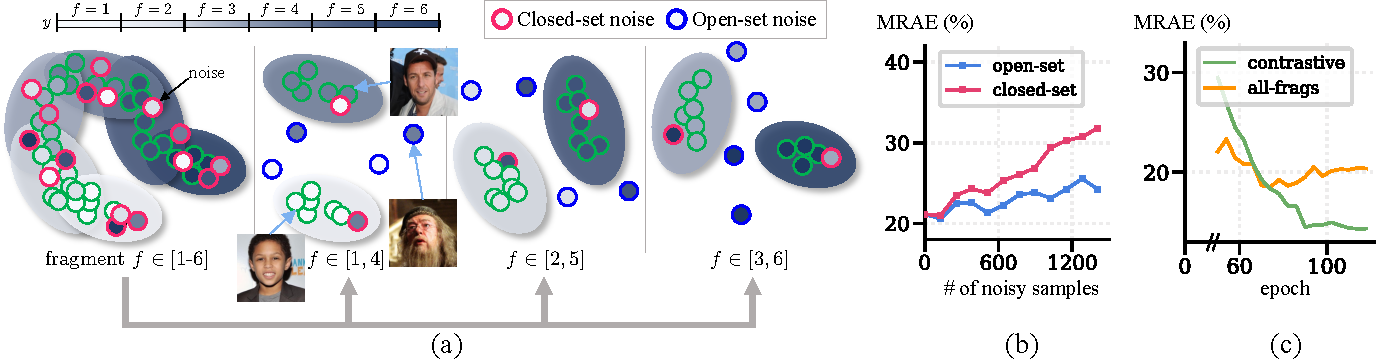
\includegraphics[width=\textwidth]{imgs/figure_1_neurips.pdf}
}
\vskip -0.15in
\caption{
(a) \textbf{An example of t-SNE illustration of contrastive fragment pairing}. 
The data with label noise are grouped into six fragments ($f\in[1\text{-}6]$) and formed into three contrastive pairs ($f\in[1, 4], [2, 5], [3, 6]$). 
% $f$ and $f^\text{gt}$ denote the fragment ids derived from the discretization of the continuous noisy labels and the ground truth labels, respectively.
Contrastive fragment pairing transforms some of \textcolor[HTML]{E73359}{closed-set noise} (whose ground truth is within the target label set) into \textcolor[HTML]{0000F5}{open-set noise} (whose ground truth is not within the label set).
% For example, in the [1,4] figure, the fragment 1 and 4 are in the closed-set, and the others are in the open-set.
For example, in the [1,4] figure, label noise whose ground truth fragment is either 1 or 4 is closed-set noise, and the others are open-set noise.
The t-SNE illustration shows that learned features of open-set noises tend to reside outside the feature clusters of the clean samples.
%Prior to contrastive fragmentation, noisy labeled data ($f\neq f^\text{gt}$) are \textcolor[HTML]{E73359}{closed-set noise} as their ground truth fragment ids are within the label set ($f^\text{gt}\in[1\text{-}6]$), and they are located in the feature spaces of incorrect classes within the group.
% After fragmentation, many noisy labeled data are easily identified as \textit{anomaly}, which can be ignored (\ie not selected) for training. 
%After contrastive fragmentation, a large portion of these noisy labeled data are transformed to \textcolor[HTML]{0000F5}{open-set noise} ($f^\text{gt}\notin[1,4]$ while $f\in[1,4]$), and they reside in an out-of-distribution feature space thus mitigating the negative effects of the noise.
% This disruption is mitigated as the noise weakens post-fragmentation, with some samples becoming anomalous (trained to reside in an out-of-distribution feature space).
(b) %When we inject closed-set and open-set noise into a clean dataset, 
The open-set noise is \textit{less harmful} with much lower errors (MRAE) in the downstream regression.
(c) The contrastive pairing ($[1, 4], [2, 5], [3, 6]$) is more effective than using all-fragments together ($[1\text{-}6]$), resulting in much lower MRAE scores.
All experiments are based on IMDB-Clean-B with more details in Appendix~\ref{subsec:contrast_combination}--\ref{subsec:disruptive_anomaly_noise}.
% (a) t-SNE Visualization of Fragmentation:
% illustrates the fragmentation process applied to the noisy data. The data is discretized into six fragments, denoted as $f\in[1\text{-}6]$, and grouped into three contrasting pairs ($f\in[1, 4], [2, 5], [3, 6]$). 
% This pairing strategy leads to the emergence of more distinctive features. Note that prior to fragmentation, the noisy labeled data can have a highly disruptive impact (as they are trained to erroneously reside in the feature space of a class that is currently being trained together). 
% However, post-fragmentation, this noise is alleviated, as some samples transform into anomalies, effectively residing in an out-of-distribution feature space.
% (b) Analysis of Different Noise Types:
% studies the impact of various noise types on downstream regression, as quantified by the Mean Relative Absolute Error (MRAE). 
% We introduce varying amounts of disruptive and anomaly noise into a clean dataset to assess their effects.
% (c) Fragment Combination Analysis:
% compares the performance of selected samples based on contrastive pairings ($[1, 4], [2, 5], [3, 6]$) against those selected from all fragments ($[1\text{-}6]$). 
% This comparison is conducted in terms of MRAE scores.
% All experiments are conducted using the IMDB-Clean-B dataset, and detailed settings can be found in Appendix~\ref{subsec:contrast_combination} and \ref{subsec:disruptive_anomaly_noise}.
}
\label{fig:fragment_motivation}
\end{center}
\vskip -0.35in
\end{figure*}
% In the noisy label regression problem, we have a dataset $\mathcal{D} = \{\mathcal{X}, Y\}$, where $(x, y)$ denotes a single sample with input $x\in\mathbb{R}^d$
% and its observed noisy label $y \in \mathbb{R}$ with the ground-truth label $y^\text{gt}$.  %The label $Y$ is a single-dimensional continuous target value.
% The goal of FragSel is to sample a subset of data denoted by $\mathcal{S} \subset \mathcal{D}$ that is clean, and thus, training upon it improves the regression performance. 
In the noisy label regression problem, we are presented with a dataset denoted as $\mathcal{D} = \{\mathcal{X}, Y\}$; in each sample $(x, y)$,  
 $x\in\mathbb{R}^d$ is an input, and $y \in \mathbb{R}$ is the observed label, which can be possibly noisy. We use  $y^\text{gt}$ to denote the groundtruth label. 
% The label $Y$ represents a single-dimensional continuous target value.
The objective of ConFrag is to sample a \textit{clean} subset of the data as $\mathcal{S} \subset \mathcal{D}$. 
By training on $\mathcal{S}$, we aim to enhance the  performance of the regression model.
% We can only observe the input $\mathcal{X}$ and its corresponding noisy label, $\tilde{Y}$, but not its true label, $Y$.
% We denote the continuous label as $\tilde{y}^c \in \tilde{Y}^c$ and its discretized label as $\tilde{y}^d \in \tilde{Y}^d$.
% TODO sw figure 3 mentions y^d creation.
% for each unique target value, a pre-designated fraction of the labels is assigned another class.

An overview of our ConFrag framework is shown in Fig.~\ref{fig:framework}(a). 
% It first fragments the dataset into \textit{contrasting fragment pairs} (\S~\ref{subsec:fragmentation}) and collectively represents them through training of feature extractors (\S~\ref{subsec:contrastive_pair_training}).
% Then, the framework probabilistically selects samples based on neighborhood agreements from $\mathcal{D}$ via a fragment-based mixture model (\S~\ref{subsec:mixture_of_contrasing_fragments}). 
% Finally, the regression model is trained on the selected data $\mathcal{S}$. % either in an online or offline manner.
% Note that FragSel does not require preliminary noise rate approximations (\ie noise rate agnostic). 
% The number of fragments $F$, $K$ for KNN-based prediction, and the jittering amount are the only hyperparameters of the framework.
% Fig.~\ref{fig:framework}(a) overviews the FragSel framework.
The framework has the following steps.
%Initially, we divide the dataset into what we refer to as \textit{contrasting fragment pairs} (\S~\ref{subsec:fragmentation}), which are collectively used for the enhanced training of feature extractors (\S~\ref{subsec:contrastive_pair_training}).
We divide the dataset into what we refer to as \textit{contrastive fragment pairs} (\S~\ref{subsec:fragmentation}), which collectively enhance the training of the feature extractors (\S~\ref{subsec:training_feature_extractors}).
We then select clean samples $\mathcal{S}$ from dataset $\mathcal{D}$ based on neighborhood agreements, utilizing a fragment-based mixture model (\S~\ref{subsec:mixture_of_contrasing_fragments}). % employ a probabilistic approach to 
% Finally, the regression task is performed by training on the selected data subset $\mathcal{S}$.
A regression model is trained on the clean samples $\mathcal{S}$.
We also propose neighborhood jittering as a regularizer for further improved training (\S~\ref{sec:jittering}).
ConFrag is noise rate-agnostic unlike prior methods as it operates without knowing a pre-defined noise rate.
% The only hyperparameters of the framework are the number of fragments denoted as $F$, the parameter $K$ used for KNN-based prediction, and the amount of jittering applied for regularization (\S~\ref{sec:jittering}).

% This design ensures that FragSel remains flexible and adaptable while achieving its core objectives.
% \subsection{Preliminary on Mixture of Experts}\label{sec:mixture_models}
% Before diving into our algorithm, we briefly review the Mixture of Experts model~\citep{jacobs1991MoE, jordan1994MoE}.
% If we let $y \in \mathbb{R}$ be an i.i.d. sample of outcome variables from a population
% modeled by a finite mixture model with $M$ components, where each $m$ is modeled by the probability density function $h_m(\cdot|\theta_m)$.
%  $\theta_m$ denotes the parameters and $\eta_m$ are the mixture weights such that $\sum_{m=1}^M\eta_m = 1$.
% The mixture of experts uniquely allows model parameters to be functions of the concomitant variables $x$.
% \begin{align}
% p(y|x) = \sum_{m=1}^M \eta_m(x) h_m(y|\theta_m(x)),
% \end{align}
% the component densities $h_m(y|\theta_m(x))$ are often coined as experts and component weights $\eta_m(x)$
% as gating networks~\citep{jacobs1991MoE}.


% \subsection{Contrastive Fragmentation}\label{subsec:fragmentation}
\subsection{Contrastive Fragment Pairing}\label{subsec:fragmentation}

\begin{wrapfigure}{r}{0.45\textwidth}
\begin{center}
\vskip -0.1in
\centerline{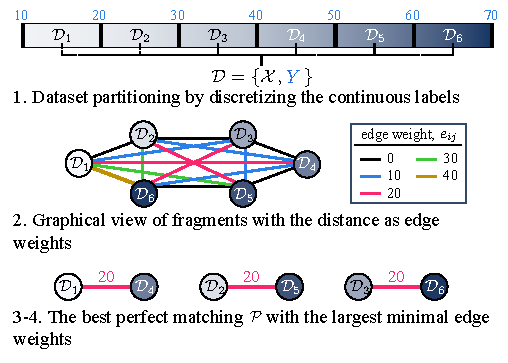
\includegraphics[width=0.5\columnwidth]{imgs/cont_fragment_neurips.pdf}}
\caption{The contrastive fragment pairing algorithm.} %The order in the figure matches the order of the algorithm in \S~\ref{subsec:fragmentation}.}
\label{fig:contrastive_fragmentation}
\end{center}
\vskip -0.3in
\end{wrapfigure}

In order to sample a \textit{clean} data subset $\mathcal{S} \subset \mathcal{D}$, 
we need to learn a robust feature that can distinguish clean samples from noisy ones.
As one theoretical result in \citep{zhang2023}, the cross-entropy loss used in classification is better for learning high-entropy feature representation than the mean squared loss in regression (see Appendix~\ref{subsec:classification_vs_regression} for details). 
Based on this, we start by discretizing the label space into $F$ continuous fragments, transforming the original regression problem into the multi-class classification one.
%High-entropy feature representations allow better separation between each fragment in representation space, allowing easier identification of noisy samples (see Appendix~\ref{subsec:classification_vs_regression}). % necessary?
This transformation harnesses an inherent property of regression: data points with similar labels are also represented with closely related features, as acknowledged in prior studies \citep{gong22rank,yang21ldsfds,yao22cmixup}.

% However, instead of training a single feature extractor on the multi-class classification with $F$ classes, we construct $F/2$ \textit{maximally contrasting fragment pairs} and train an expert feature extractor for each pair, whose size in terms of the number of parameters is smaller than the single feature extractor.
However, instead of training a single feature extractor on the multi-class classification with $F$ classes, we construct $F/2$ \textit{maximally contrasting fragment pairs} and train a smaller expert feature extractor for each pair.
The procedure of contrastive fragment pairing is detailed below with an illustration in Fig.~\ref{fig:contrastive_fragmentation}:

\begin{enumerate}[leftmargin=*]
\item Divide the range of continuous labels $Y$ into $F$ even number of equal-length fragments.
  This allows to divide the dataset $\mathcal{D}$ into $F$ disjoint subsets: $\mathcal{D} = \{\mathcal{D}_1, ... ,\mathcal{D}_F \}$, where 
%   The discrete labels $\tilde{Y}^d$ are formed here by mapping each $\tilde{y}^c$ to its corresponding fragment, $\mathcal{D}_i$. 
    each $\mathcal{D}_i$ contains the data samples whose $y$ values are in the $i$-th fragment label range. % all the data samples, $\{\mathcal{X}_i, \tilde{Y}_i^d, \tilde{Y}_i^c\}$ within the $i$-th fragment range.
    % \item Drop fragments that have less than $\tau$ number of samples.
\item Construct a complete graph $g= \{\mathcal{D}, E\}$, where each vertex is a  fragment $\mathcal{D}_i$, and each edge weight $e_{ij}$ is the distance in the label space between the closest samples of the fragments $(\mathcal{D}_i,\mathcal{D}_j)$. 
\item Compute all possible \textit{perfect matchings}~\citep{monfared16pm, gibbons85pm}, where every vertex of a graph is incident to exactly one edge in the graph.  
    %Formally, $\bar{g}=\{\mathcal{F}, \bar{E}\}$ is a perfect match when $|\bar{E}| =\frac{1}{2}|\mathcal{F}|$ and $M=\frac{1}{2}|\mathcal{F}|$ where $M$ is the matching number, $|\cdot|$ indicates the size of the set. graphs, $\bar{g}$ and store into $\mathcal{G}$.
%    Note that the perfect matching constraint requires an even number of vertices. Hence the reason for the number of fragments $F$ to be even in step 1.
    % of $G := \{\Phi, E\}$. %with unique set of $E$.
    % \begin{align}\label{eq:permuations}
    %       P = \binom{\Phi}{k}
    %     % P = \{ \forall \{\phi_n, \phi_m\} \in \Phi \}
    %     P = \{ p \in \Phi | |p| = 2\}
    % \end{align}
    % where $k$ is fixed to 2 in this work.
\item Find the perfect matching with the largest minimal edge weight: %fragment pairs by solving the optimization problem 
    %\begin{align}\label{eq:fragment}
        $\mathcal{P} = \argmax_{\bar{g}\in \mathcal{G}}\Bigl(\min\nu(\bar{g})\Bigr)$,
    %\end{align}
    % under the perfect matching constraint that all $\phi$s must be considered. %$P$ is the set of permuted pairs of $\Phi$, 
    where each $\bar{g}$ is a perfect matching (graph), and  $\nu(\bar{g})$ is the set of edge weights in $\bar{g}$.
% By maximizing the minimal distance within the permuted set of fragments, we maximize the overall gap between fragments, 
Finally, $\mathcal{P}=\{ (\mathcal{D}_i, \mathcal{D}_j), \ldots ,(\mathcal{D}_k, \mathcal{D}_l)\}$ constitutes the \textit{maximally contrasting pairs} of fragments. %where $i,j,k,l$ are arbitrary indices of the fragments.
% The Appendix shows that pairs are the optimal fragment group that maximizes the distances between the fragments.
\end{enumerate}


%\textbf{Theoretical justification}.  
\textbf{Motivation behind contrastive fragment pairing. }
Formulating the multi-class classification problem into $F/2$ binary classification problems via contrastive fragment pairing has the following advantages.
%, which help achieving better performance than training single feature extractor as shown in Fig.~\ref{fig:fragment_motivation}(c).
% Firstly, the distance between fragments in each contrastive fragment pair is large, and so is the margin of the classifier on training points.
% Firstly, the distance between fragments in each contrastive fragment pair is large, and so would be the margin of training points (input margin) and margin of their features (feature margin).
% Firstly, since the distance between fragments in each contrastive fragment pair is large, we naturally expect the distance of data points between two fragments to be large as well.
% Theoretically and empirically, a larger margin results in a better generalization bound \citep{shawe1998robust, gronlund2019margin, gronlund2020near, mouton2024input}.
% Theoretically and empirically, a larger distance (margin) results in a better generalization \citep{shawe1998robust, gronlund2019margin, gronlund2020near, mouton2024input}.
Firstly, since the distance between fragments in each contrastive fragment pair is large, the feature extractor trained on each contrastive pair can generalize better \citep{shawe1998robust, gronlund2019margin, gronlund2020near}.
% We empirically observe that this applies in our framework too, as shown in Fig.~\ref{fig:fragment_motivation}(c).
Fig.~\ref{fig:fragment_motivation}(c) shows the generalization abilities of the expert feature extractors trained on contrastive fragment pairs compared to the single feature extractor trained on all fragments.
When using a single feature extractor on all fragments (all-frags), the samples selected by the feature extractor tend to become more noisy as the feature extractor overfits, causing the regressor to perform worse over time.
On the other hand, when using multiple feature extractors trained on contrastive pairs, the performance of the regression model consistently improves, indicating that the learned features are more robust and the selected samples are cleaner.
% As shown in Appendix~\ref{subsec:contrast_combination}, a large margin on training points also explains why maximally contrasting fragment pairing is superior to other fragment pairings.
% As shown in \S~\ref{sec:discussion}, a large margin on training points also explains why maximally contrasting fragment pairing is superior to other fragment pairings.
The large distance between fragments also explains why contrastive fragment pairing is superior to other fragment pairings, as shown in \S~\ref{sec:discussion}.
The analysis of the prediction depth \citep{baldock21nips} in Appendix~\ref{subsec:prediction_depth_analysis} supports the claim, as it shows that the binary classification on contrastive fragment pairs results in lower prediction depth, leading to better generalization.
% For detailed comparison between maximally contrasting fragment pairing and other fragment pairing, see Appendix~\ref{subsec:contrast_combination}
% \textbf{[Explanation related to MoE? + why maximally contrasting pairs is important? want: binary classification with distant classes leads to less memorization and thus more robust feature (has similar observation in appendix, where contrastive pair is better than e.g., [1,2], [3,4], [5,6]]}.
% as in MoE, each expert can then be mixed together to outperform a single network trained using the entire dataset
% consider case where in MoE, the subtask is already known.
% for now, first try exploring the "memorization" option

Secondly, the contrastive fragment pairing transforms some of \textit{closed-set} label noise (whose ground truth is within the label set) into \textit{open-set} label noise (whose ground truth is not within the label set), as shown in Fig.~\ref{fig:fragment_motivation}(a).
Previous works \citep{wei2021open, wan2024unlocking} observe that the open-set noise is less harmful than the closed-set noise and may even benefit generalization and robustness against inherent noisy labels.
Indeed, in our experiments, we found similar observations where injecting open-set label noise is less harmful than closed-set one, as shown in Fig.~\ref{fig:fragment_motivation}(b).

The t-SNE visualization in Fig.~\ref{fig:fragment_motivation}(a) also supports this observation.
Let $f$ and $f^\text{gt}$ be fragments that the observed label $y$ and the groundtruth label $y^\text{gt}$ respectively belong to.
Prior to contrastive fragment pairing, all of the noisy labeled data ($f\neq f^\text{gt}$) are \textcolor[HTML]{E73359}{closed-set noise} as their ground truth fragment ids are within the label set ($f^\text{gt}\in[1\text{-}6]$) and their features %learned by the single feature extractor 
are located in the feature spaces of incorrect classes within the group.
After contrastive fragment pairing, much of these noisy labeled data is transformed to \textcolor[HTML]{0000F5}{open-set noise} ($f^\text{gt}\notin[1,4]$ while $f\in[1,4]$ in case of fragment pair $[1, 4]$), 
% and their learned features tend to reside in an out-of-distribution feature space thus mitigating the negative effects of the noise.
and their learned features tend to reside outside the feature clusters of the clean samples, thus mitigating the adverse effects of the noise.

%\subsection{Training  Feature Extractors for Contrastive Pairs}\label{subsec:contrastive_pair_training}

\subsection{Training  Feature Extractors for Contrastive Pairs}
\label{subsec:training_feature_extractors}

% Once we obtain $\mathcal{P}$, we train $F/2$ number of expert feature extractors, each of which, denoted as $p(y|x;\theta_{i,j})$ with parameters $\theta_{i,j}$, is a binary classifier for every contrastive pair $(\mathcal{D}_i, \mathcal{D}_j) \in \mathcal{P}$. That is, it is trained to predict whether a data is in $\mathcal{D}_i$ or $\mathcal{D}_j$.
% Once we obtain the contrastive fragment pairs $\mathcal{P}$, we train $F/2$ number of expert feature extractors, each of which, denoted as with parameters $\theta_{i,j}$, is trained on binary classification $p(y|x;\theta_{i,j})$ with its respective contrastive pair $(\mathcal{D}_i, \mathcal{D}_j) \in \mathcal{P}$.
Once we obtain the contrastive fragment pairs $\mathcal{P}$, we train $F/2$ number of expert feature extractors on binary classification $p(y|x;\theta_{i,j})$ with its respective contrastive pair $(\mathcal{D}_i, \mathcal{D}_j) \in \mathcal{P}$, where $\theta_{i,j}$ denotes the parameter of an expert.
That is, it is trained to predict whether a data $x$ is in $\mathcal{D}_i$ or $\mathcal{D}_j$.
% Later, the feature extractors play a crucial role in generating predictive/representational features for each fragment. 
Later, the feature extractors play a crucial role in determining whether a sample $(x, y)$ is clean.

\begin{figure}[t]
\begin{center}
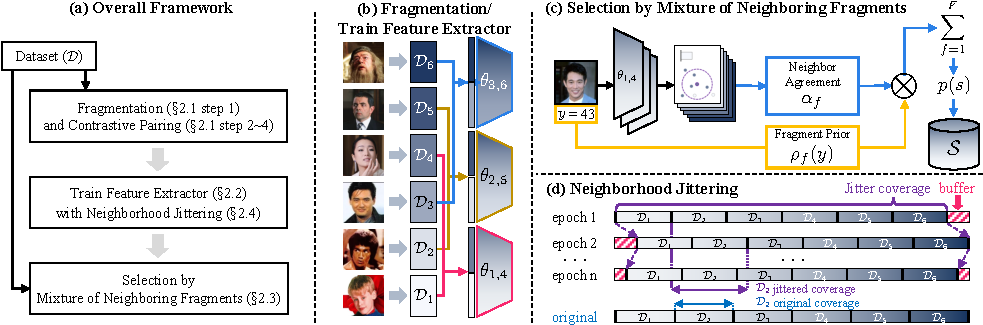
\includegraphics[width=\textwidth]{imgs/main_framework_simplified.pdf}
\caption{\textbf{Contrastive Fragmentation framework.}
% The framework takes as input data with
% continuous labels such as age prediction or clothing price prediction.
(a) The overall sequential process of our framework.
% (b) Shows the fragmentation of the continuous label space to obtain \textit{contrasting fragment pairs} and train feature extractors on them (\S~\ref{subsec:fragmentation}).
(b) Shows the fragmentation of the continuous label space to obtain \textit{contrasting fragment pairs} (\S~\ref{subsec:fragmentation}) and train feature extractors on them.
% (b) Shows the fragmentation of the continuous label space (\S~\ref{subsec:fragmentation}) to obtain \textit{contrasting fragment pairs} and train feature extractors on them (\S~\ref{subsec:contrastive_pair_training}).
(c) Sample Selection by Mixture of Neighboring Fragments obtains the selection probability in both prediction and representation perspectives (\S~\ref{subsec:mixture_of_contrasing_fragments}).
(d) Illustration of Neighborhood Jittering (\S~\ref{sec:jittering}).
}
\label{fig:framework}
% include the notion of creating most contrasting (distant) fragments into the diagram
% put big big emphasis on NEIGHBOR agreement in the prediction and feature space
\end{center}
\vskip -0.2in
\end{figure}




\subsection{Mixture of Neighboring Fragments}
\label{subsec:mixture_of_contrasing_fragments}

With the learned expert feature extractors, the next step is to perform sample selection.
Given a sample $(x, y)$, let $f$ be a fragment close to $y$ and $f^+$ be its contrasting pair.
Intuitively, we consider a sample clean if the expert trained on $(\mathcal{D}_f, \mathcal{D}_{f^+})$ strongly predicts that $x$ belongs to a fragment $f$.
However, since the expert feature extractor is a binary classifier only trained using a contrasting pair of fragments, we utilize all experts' opinions to obtain a more robust prediction. % (\ie, mixture of neighboring experts).
% Intuitively, we want to select sample $(x, y)$ that belongs to a fragment that is close to $y$.
% Specifically, to deem a sample as clean, closer a fragment $f$ is to $y$ (\textbf{Fragment Prior}), more strongly the expert trained on the fragment $f$ contributes to prediction as encouraging the consensus (\textbf{Neighborhood Agreement}).
% Specifically, closer a fragment $f$ is to $y$ (\textbf{Fragment Prior}), more strongly the expert trained on the fragment $f$ contributes to the prediction (\textbf{Neighborhood Agreement}).
% Specifically, we deem a sample as clean if for a fragment $f$ close to $y$ (\textbf{Fragment Prior}), the experts in its neighborhood should exhibit a consensus response (\textbf{Neighborhood Agreement}).
Specifically, we deem a sample as clean if the experts exhibit a consensus response (\textbf{Neighborhood Agreement}) for fragments close to $y$ (\textbf{Fragment Prior}).

%Based on this intuition, we formulate Mixture model, where we define the sampling probability as
Based on this intuition, we formulate Mixture of Experts (MoE) \citep{jacobs1991MoE} model, where the sampling probability of a datapoint $(x, y)$ is defined as
%Our sample selection based on neighboring experts is formulated by a Mixture of Experts \citep{jacobs1991MoE}, where we define the sampling probability of data $(x, y)$ as 
\begin{align}\label{eq:mcf}
    % p^{p/r}(s|x,\mathcal{D}_{1 \ldots F};\Theta) &= \sum_{f}^{F} \eta_f(\tilde{y}^c)\alpha_f(x, \tilde{y}^c; \mathcal{D}_{1 \ldots F}, \Theta)
    p(s|x,y, \mathcal{D}_{1 \ldots F};\Theta) &= \sum_{f}^{F} \rho_f(y)\alpha_f(x; \mathcal{D}_{1 \ldots F}, \Theta),
\end{align}
where $\Theta$ denotes parameters of all  feature extractors, $\rho_f$ is the \textit{fragment prior} (mixture weight), and $\alpha_f$ is the \textit{neighborhood agreement} (a binary vote  of whether $x$ belongs to the fragment $f$).
Based on the intuition above, $\rho_f(y)$ is large when the fragment $f$ is close to $y$, and $\alpha_f(x) \in \{0, 1\}$ is $1$ if $x$ is likely to belong to the fragment $f$.% and its neighboring fragments.

\textbf{Fragment Prior.}
For a sample $(x, y)$, we compute the prior $\rho_f(y)$ of a fragment $f$,
using a softmax weighting of each fragment $f$ with respect to its relative distance to $y$:
\begin{align}\label{eq:np}
    \rho_f(y)=\frac{\exp(g_f(y))}{\sum_{f'}^F \exp(g_{f'}(y))}, %\hspace{6pt} \text{where }  g_f(y)=\frac{\max(Y) - \min(Y)}{|y - \bar{Y}_f|}.
%    \eta &= \left\{\text{softmax}\left( \bigcup^F_f \frac{\max(\tilde{Y}^c) - \min(\tilde{Y}^c)}{|\tilde{y}^c - \bar{Y}^c_f|}\right)\right\}_f
\end{align}
where $g_f(y)=\text{range}(Y)/ (|y - \bar{Y}_f|)$, $\text{range}(Y)=\max(Y) - \min(Y)$ is the label range, and $\bar{Y}_f$ is the mean label value of fragment $f$.
Since $\text{range}(Y)$ is a constant for a given dataset, $g_f(y)$ rapidly decreases when the mean value of fragment $f$ is far from $y$ in the continuous label space.
From the MoE perspective, the fragment prior can be regarded as soft gating that depends on $y$.

\textbf{Neighborhood Agreement.}
% 
%Given a sample $(x, y)$ and a fragment $f$, we classify whether $x$ belongs to $f$ using the expert that is trained using $(\mathcal{D}_f, \mathcal{D}_{f^+})$ where $f^+$ is contrasting fragment of $f$.
Given a sample $(x, y)$ and a fragment $f$, we need to determine whether $x$ belongs to $f$.
% The simplest approach is to use the expert trained using $(\mathcal{D}_f, \mathcal{D}_{f^+})$ where $f^+$ is contrasting fragment of $f$, to classify whether $x$ belongs to $f$ or $f^+$.
The simplest approach is to use the expert trained using $(\mathcal{D}_f, \mathcal{D}_{f^+})$ to classify whether $x$ belongs to $f$ or $f^+$, where $f^+$ is the contrasting fragment of $f$.
% Based on the classification output, we define self-agreement as
Based on the classification output $h(x; \theta_{f, f^+}) \in \{f, f^+\}$, we define self-agreement as:
%We utilize two aspects of the expert.
%First is predictive aspect, where we use the binary classifier learned during the training of the expert in \S~\ref{subsec:training_feature_extractors}, which is a linear classifier on the learned feature space.
%Second is representational aspect, where we use non-linear k-nearest neighbor classifier on the feature space learned by the expert.
% By utilizing both linear and non-linear classifier on the same feature space, we can obtain more robust classification.
%The classification result, which we call self-agreement, is computed as:
%\begin{align}
%    \alpha^\text{self}_f = 
%    \begin{cases}
%        [h(x; \theta_{f, f^+}) == f] & \hspace{-6pt}\text{\small : predictive} \  \\
%        [\text{vote}(K_x) == f] & \hspace{-6pt}\text{\small : representational} \ 
%    \end{cases}\label{eq:self_agreement}
%\end{align}
\begin{align}
   \alpha^\text{self}_f = 
       [h(x; \theta_{f, f^+}) = f] % & \hspace{-6pt}\text{\small : predictive}
\label{eq:self_agreement}
\end{align}
% where $\theta_{f, f^+}$ is the expert model parameter, $h(x; \theta_{f, f^+})$ is the output of the feature extractor's binary classifier, $K_x$ is the label list (fragment ids) of $k$-nearest neighbors of $x$ from $(\mathcal{D}_f, \mathcal{D}_{f^+})$ in the representation space, and $\text{vote}(\cdot)$ is a voting function that output most frequent item in the given list.
% where $h(x; \theta_{f, f^+})$ is the classification output, and $[A]$ is the Iverson bracket which outputs $1$ if $A$ is true, and 0 otherwise.
where $[A]$ is the Iverson bracket outputting $1$ if $A$ is true, and 0 otherwise.
% \textbf{[WIP: why discrete output rather than continuous probabilistic output?]}
% We use discrete classification output rather than continuous probabilistic one to avoid sampling noisy samples, even with small probability.
% Since training with noisy labels often results in suboptimal calibration \citep{bae22icml, joel2023effect}, we use discrete classification output rather than continuous probabilistic one.
Since training with noisy labels often results in suboptimal calibration \citep{bae22icml, zong2024dirichlet}, we use discrete classification output for $\alpha^\text{self}_f$ rather than continuous probabilistic one.

%However, since training with noisy labels often results in suboptimal calibration~\citep{bae22icml}, we mitigate its effects via an ensemble of neighboring experts.
Since the expert $\theta_{f, f^+}$ is only trained to discriminate between $f$ and its contrasting fragment $f^+$, it is better to utilize other experts to obtain a more robust prediction.
For example, consider contrastive fragment pairs $\{(1,4), (2,5), (3,6)\}$ as in Fig.~\ref{fig:contrastive_fragmentation}.
If $x$ is more likely to belong to fragment $2$ than $5$, then it should be more likely to belong to $1$ than $4$ and $3$ than $6$.
Thus, we consider agreement of neighboring fragments $f_L$ (left) and $f_R$ (right) to obtain neighborhood agreement $\alpha_f(x; \mathcal{D}_{1 \ldots F}, \Theta)$:
\begin{align}
  \alpha_f(x; \mathcal{D}_{1 \ldots F}, \Theta) = \alpha^\text{self}_f \cdot \alpha^\text{ngb}_f, \hspace{3pt} \text{ where} %\label{eq:na_final} 
    \ \ \alpha^\text{ngb}_f = \left[ \alpha^\text{self}_{f_L} \lor \alpha^\text{self}_{f_R} \right]. \label{eq:na_final}    
\end{align}
% Intuitively, $\alpha_f$ is $1$ if the fragment $f$ is more likely for $x$ than its contrasting pair $f^+$ ($\alpha^\text{self}_f = 1$) and either $f$'s left or right fragment is more likely for $x$ than its contrasting pair ($\alpha^\text{ngb}_f = 1$).
Intuitively, $\alpha_f$ is $1$ if the fragment $f$ is more likely for $x$ than $f^+$ ($\alpha^\text{self}_f = 1$) and either $f$'s left or right fragment is more likely for $x$ than its respective contrasting fragment ($\alpha^\text{ngb}_f = 1$).

% By considering the neighborhoods and their agreements based on predictive and representational aspects of the feature extractors,
% we obtain two types of sample probability in Eq.(\ref{eq:mcf}): predictive $p^p(\cdot)$, based on the feature extractors' binary classification, and representational $p^r(\cdot)$, based on k-nearest neighbor classification on the learned feature spaces. %, whose differences lies in how to compute $p(f|x)$ in Eq.(\ref{eq:score}).
% Subsequently, we respectively sample $\mathcal{S}^p$ and $\mathcal{S}^r$ from $p^p(\cdot)$ and $p^r(\cdot)$.
% Finally, the \textit{clean} data subset $\mathcal{S}$ is the union of $\mathcal{S}^p$ and $\mathcal{S}^r$.
% Algorithm~\ref{alg:fragmented_selection} in the Appendix provides the overall pseudocode.
% In practice, we use different classification approach for Eq.(\ref{eq:self_agreement}) to obtain respective sample probability $p(s|x, y)$, and use the union of the sampled clean data subset.
In practice, we implement two variants of the agreements in Eq.(\ref{eq:self_agreement}--\ref{eq:na_final}) using the feature extractor's binary classifier and a $K$-nearest neighbor classifier on the learned feature space.
These two classifiers respectively consider \textit{predictive} and \textit{representational} aspects of the expert feature extractor and effectively work as an ensemble, as shown in Appendix~\ref{subsec:ablation}.
As a result, we compute two versions of sample probability in Eq.(\ref{eq:mcf}), and use the union of the sampled \textit{clean} dataset $\mathcal{S}$ for training of the regression model. 
Algorithm~\ref{alg:fragmented_selection} in Appendix summarizes the overall procedure.


\subsection{Neighborhood Jittering}\label{sec:jittering}


\begin{figure*}[t]
\begin{center}
\centerline{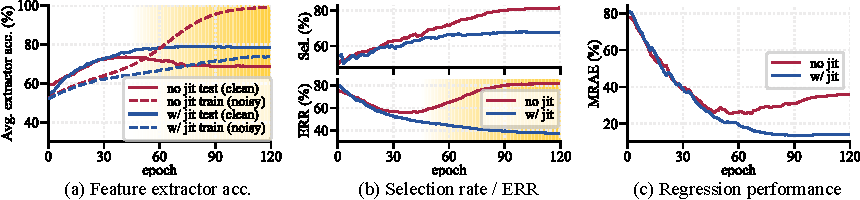
\includegraphics[width=1.0\textwidth]{imgs/jitter_analysis_neurips.pdf}}
\vskip -0.1in
\caption{\textbf{Jittering analysis.}
(a) When trained without jittering, feature extractors easily overfit the noisy training data (yellow-shaded region), while jittering-regularized feature extractors robustly learn from the noisy training data. %and maintain high accuracy on clean test data.
(b) Overfitted feature extractors (yellow-shaded region) on noisy samples increase their likelihood, leading to a higher selection rate and ERR. 
It exhibits nearly twice higher ERR (a lower value is better).
(c) Most importantly, jittering regularization improves performance in regression.
% The analysis is done on IMDB-Clean-B with symmetric 40\% noise, both with and without an additional 5\% buffer range jittering.
% (a) Top: ratio of [clean/noisy samples with $\alpha_f=1$: total clean/noisy samples]. Bottom: ERR of noisy samples with $\alpha_f=1$.
% (b) Mean discriminator train/test accuracy with or without 5\% buffer range jittering.
% (c) ERR of selected samples, ($\mathcal{S}$) with or without 5\% buffer range jittering. 
% The analysis is conducted on IMDB-Clean-B with symmetric 40\% noise, %, where experiments are based on the best-performing epoch.
% and for (b,c) none other regularizations are applied for feature extractor training.
}
\label{fig:jitter_analysis}
\end{center}
\vskip -0.2in
\end{figure*}

A potential limitation of mixture models is that the individual expert feature extractor may not fully benefit from the full dataset as they model their own disjoint subsets~\citep{dukler23}.
Our neighborhood jittering mitigates this limitation as a robust regularizer that expands the effective coverage of each contrastive fragment pair during learning.
The process is visualized in Fig.~\ref{fig:framework}(d).

We bound the ratio of the jittering buffer range  within $[0, \frac{1}{2(F-1)}]$, where $F$ is the fragment number.
For every epoch, we shift the label coverage of each fragment by randomly sampling the value in this range. %This leads to an increased label coverage for the fragments.
% and the maximal boundary defines the stop range to prevent the overlap of mixtures.
%We restrict the ratio of the buffer range to jitter within to the interval  $[0, 1/2(F-1)]$, where $F$represents the number of fragments, and the upper boundary serves as the stop range to prevent overlap between mixtures.
% Consequently, for each epoch, we shift the coverage of labels in the dataset by a randomly sampled value from within the buffer range.
% This resultantly has a similar effect as bagging~\citep{}, which regularizes by training multiple models(ensembles) by creating subsets that are sampled with replacement from the full dataset. 
% But, jittering within the maximally allowed boundary for mixture models to attain a similar effect.
% Jittering leads to a partially overlapping mixture model~\citep{heller07, hinton02poe} as the effective coverage per mixture is increased and some data belong to multiple mixtures \ie neighboring fragments.
Jittering leads to a partially overlapping mixture model~\citep{heller07, hinton02poe} as some data belong to multiple, neighboring fragments and thus the effective coverage per each expert is expanded.
% Given that FragSel's effectiveness hinges on neighbor agreements, the jittering or overlapped training naturally improves the learning of neighboring fragments to discern the sample selection during Neighborhood Agreeability (\S~\ref{subsec:mixture_of_contrasing_fragments}).
% Since FragSel's effectiveness hinges on neighbor agreements, the jittering-induced overlap in training enhances learning of neighboring fragments (\S~\ref{subsec:mixture_of_contrasing_fragments}).
% Fig.~\ref{}(a,b) shows that the overall selected sample ($\mathcal{S}$) error is reduced with jittering. % I think this is not related with next paragraph, which says that jittering is good because it avoids overfitting. 
% This is due to the neighbor agreement ($\alpha_f$) increasing for the clean samples slightly while the noisy samples' neighbor agreement decreases by a large margin.
%the clean sample neighbor agreement ($\alpha_f=1$) ratio is not negatively impacted.
Such regularization inhibits feature extractors from overfitting to potentially noisy samples and promotes learning of more robust features, even those that can be generalizable to overlapping parts of neighboring fragments.

Fig.~\ref{fig:jitter_analysis}(a) shows that with jittering, the feature extractor exhibits higher accuracy on the clean test data due to its regularization effect. 
In the sample selection stage (Fig.~\ref{fig:jitter_analysis}(b)), 
the feature extractor trained without jittering easily overfits the noise, resulting in over-selection and higher ERR (\S~\ref{subsec:evaluation_metrics}). 
%the feature extractor trained without jittering easily overfits the noise, resulting in high ERR along with high selection rate, indicating that noisier samples are being selected.
In contrast, the jittered feature extractor achieves a relatively low selection rate with halved ERR, indicating that the noisier samples are filtered out.
% In contrast, the jittered feature extractor achieves a relatively low selection rate with halved ERR, indicating that the selected samples are cleaner.
% In contrast, the jittered feature extractor achieves nearly halved ERR and lower selection rate, indicating that the selected samples are cleaner and noisier samples are being filtered out.
Better sample selection due to jittering subsequently leads to significantly better performance in regression (Fig.~\ref{fig:jitter_analysis}(c)).
% Lastly, as shown in Fig.~\ref{fig:jitter_analysis}(d), jittering leads to significantly better performance in regression.
% In Appendix~\ref{subsec:hyperparameter} and \ref{subsec:jitter_comparison}, we provide the performance variation according to the amount of jittering and compare to other regularizations, demonstrating its efficacy.
In Appendix~\ref{subsec:jitter_comparison}, we compare neighborhood jittering to other regularizations, demonstrating its efficacy.

% Fig.~\ref{fig:jitter_analysis}(b) shows that t jittering enhances the overall precision of selected samples; the neighbor agreement of noisy samples decreases significantly, whereas that of clean samples remains relatively stable. %\ie jittering improves the overall precision of the selected samples.
% This is further veried by the substiantial ERR decrease on the bottom graph.
% In Fig.~\ref{fig:jitter_analysis}(a,c), the model tends to overfit more easily in the absence of jittering, resulting in a higher ERR for the selected data. Conversely, the inclusion of jittering allows us to achieve significantly lower error rates.

% One main type of synergetic effect would be the similar features such as those in the similar label neighborhood. Jittering is able to offer this.
% By allowing each contrastive fragment pair to cover more range, it also allows to view more diverse data at each epoch, also leading to overfitting mitigation.
% search for overfitting and noisy label relation? Overfitting to noise destroys the embeddings and likelihood.
% mitigates MoE's disadvantage of losing the synergetic data effect of the full dataset by covering partitioned areas.
% jittering mitigates the synergetic data effect by increasing the coverage of learned data
% jittering mitigates overfitting.
% jittering is unique to continuous data
% jittering mitigates the overfitting effect of the discriminative model by increasing the coverage of the learned data, as well as introducing jitter.


\section{Related Works}\label{sec:related_works}
\vskip -0.05in
We review prior works on learning with noisy labels and defer a comprehensive survey to Appendix \ref{subsec:related_work}. % of continuously ordered correlation of labels and features
% As vibrant as the research is in learning with noisy labels, there are multiple research directions.
% We organize them into those exploring prediction, representation, and combination of the two.
We organize them into those utilizing prediction, representation, and combination of the two.

\textbf{Prediction-based Methods}.
This approach has been the focus of much existing research and covers a wide array of topics: (i) 
the small loss selection by exploring the pattern of memorization in neural networks~\citep{han18coteaching, arazo19}, 
(ii) relying on the consistency of predictions to select or refurbish the samples~\citep{liu2020early,huang2020self},
(iii) estimating the noise distribution~\citep{patrini17,hendrycks18nips},
(iv) introducing auxiliary parameters or labels~\citep{pleiss20aum,hu20rdiaux},
(v) using unlabeled data with semi-supervised learning~\citep{li2020dividemix,bai2021understanding,karim2022unicon}, 
and (vi) designing a noise-robust loss function~\citep{menon20phuber,wang19sce}.

\textbf{Representation-based Methods}.
This approach has seen a recent surge in interest, including
(i) clustering based selection~\citep{mirzasoleiman20crust,wu20topo},
(ii) feature eigendecomposition filtering~\citep{kim21fine}, %framing the noisy labeled as outliers~\cite{wang18}, 
(iii) using neighbor information to sample and refurbish with clean validation~\citep{li22neighbor, gao16knn},
and (iv) generative models of features for sampling~\citep{kmlee19}.

\textbf{Combination}.
Some works have also studied the combination of representation and prediction spaces.
\citet{wang22spr} formulate a penalized regression between the network features and the labels for selection,
and \citet{ma18d2l} use intrinsic dimensionality and consistent predictions to refurbish.
% \textcolor{magenta}{Moreover, \citet{wu2021ngc} expands the scope of the noisy label problem to a broader open-world scenario, and addresses it through a noisy graph cleaning framework.}
Other important approaches include (i) regularization via MixUp~\citep{zhang18mixup} along with its regression version~\citep{yao22cmixup},
(ii) model-based methods that discourage large parameter shifts~\citep{hu20rdiaux}, and (iii) importance discrimination of parameter updates~\citep{xia21cdr}.
%In accordance, our approach simultaneously employs the agreement of neighbors in the prediction and representation spaces for sample selection.

The majority of previous works have studied noisy labels for classification. Hence, a large portion of these works may not be directly applicable to regression tasks due to the restricted usage of class-wise information. % or the requirement of a likelihood distribution derived from the softmax output.
In \S~\ref{sec:experiments}, we empirically compare our method with some of these works that are expandable to the regression task with some or minor technical adaptation.

\begin{table*}[th!]
    \caption{\textbf{Comparison of Mean Relative Absolute Error (\%)} over the noise-free trained model on the AFAD-B, IMDB-Clean-B, IMDB-WIKI-B, SHIFT15M-B, and MSD-B datasets.
    Lower is better. A negative value indicates it performs even better than the noise-free model.
    The results are the mean of three random seed experiments.
    The best and the second best methods are respectively marked in \textcolor{red}{red} and \textcolor{blue}{blue}.
    %FragSel/FragSel-R refers to classification/regression-based feature extractors.
    CNLCU-S/H, Co-Selfie, and Co-ConFrag use dual networks to teach each other as done in \citet{han18coteaching}.
    SPR~\citep{wang22spr} fails to run for SHIFT15M-B due to excessive memory usage.}
    %\vskip -0.15in
    \begin{center}
    \begin{small}
    \setlength{\tabcolsep}{2.0pt}
    \begin{tabular}{lccccccccccccc}
        \toprule
        &\multicolumn{6}{c}{AFAD-B}       &\multicolumn{6}{c}{IMDB-Clean-B}& IMDB-WIKI-B
        \\\cmidrule(lr){2-7}\cmidrule(lr){8-14}
        &\multicolumn{4}{c}{symmetric}    &\multicolumn{2}{c}{Gaussian} &\multicolumn{4}{c}{symmetric} &\multicolumn{2}{c}{Gaussian} & real noise
        \\\cmidrule(lr){2-5}\cmidrule(lr){6-7}\cmidrule(lr){8-11}\cmidrule(lr){12-13}\cmidrule(lr){14-14}
        %\midrule
        noise rate  & 20 & 40 & 60 & 80 & 30 & 50 & 20 & 40 & 60 & 80 & 30 & 50 & - \\
        \midrule
        Vanilla & 9.37  & 20.27 & 30.65 & 43.09 & 28.77 & 39.03 & 16.18 & 32.05 & 53.13 & 76.35 & 26.89 & 50.28 & 0 \\
        \specialrule{0.1pt}{1pt}{1pt}
        CNLCU-S   & 10.98 & 20.44 & 32.44 & 41.99 & 30.60 & 40.66 & 51.40 & 66.62 & 82.83 & 85.65 & 83.39 & 82.10 & 21.54 \\
        CNLCU-H   &  4.63 & 16.32 & 36.01 & 44.71 & 35.68 & 43.64 & 6.84 & 31.16 & 63.08 & 82.65 & 46.53 & 65.24 & -2.93 \\
        Sigua     &  5.96 & 21.09 & 43.33 & 49.71 & 42.52 & 46.19 & 9.82 & 46.17 & 77.59 & 85.62 & 60.97 & 77.42 & 1.96 \\
        SPR       &  9.74 & 18.85 & 30.43 & 43.25 & 28.50 & 39.69 & 14.47 & 32.44 & 54.88 & 79.37 & 25.67 & 51.05 & -0.93 \\
        BMM       &  5.60 & 15.00 & 39.15 & 46.41 & 30.96 & 44.00 & 8.85 & 21.54 & 55.57 & 80.40 & 24.33 & 57.21 & 17.88 \\
        DY-S      &  6.87 & 15.56 & 32.24 & 45.72 & 24.40 & 43.41 & 10.42 & 21.90 & 49.94 & 78.16 & 24.70 & 44.56 & -3.41 \\
        C-Mixup   & \textcolor{blue}{2.74} & 14.80 & 27.17 & 41.95 & 24.28 & 36.91 & 8.82 & 27.74 & 50.87 & 76.79 & 21.92 & 47.04 & \textcolor{blue}{-5.26} \\
        RDI       & 10.64 & 21.80 & 39.32 & 47.07 & 37.33 & 44.41 & 16.35 & 29.33 & 55.91 & 79.92 & 25.69 & 51.35 & 1.06 \\
        CDR       & 10.26 & 18.71 & 32.27 & 43.38 & 29.74 & 39.21 & 17.47 & 32.19 & 54.75 & 75.45 & 28.46 & 51.73 & -0.39 \\
        D2L       &  9.43 & 20.75 & 31.25 & 44.50 & 28.86 & 40.10 & 16.94 & 33.85 & 55.54 & 76.28 & 29.30 & 52.44 & -0.66 \\
        AUX       &  6.15 & 19.01 & 31.16 & 42.83 & 28.28 & 39.05 & 12.58 & 28.82 & 52.33 & 76.75 & 23.27 & 49.42 & -3.67 \\
        Selfie    & 16.91 & 25.02 & 44.18 & 47.78 & 46.02 & 50.73 & 27.43 & 53.74 & 79.38 & 84.00 & 60.68 & 78.03 & 14.00 \\
        Co-Selfie & 14.61 & 22.95 & 39.79 & 47.72 & 41.05 & 53.00 & 23.52 & 50.07 & 67.42 & 84.25 & 52.44 & 74.73 & -0.44 \\
        Superloss &  7.36 & 18.24 & 29.78 & 44.26 & 27.59 & 42.96 & 23.38 & 45.41 & 67.11 & 80.85 & 53.88 & 63.33 & -3.58 \\
        % OrdRegr & 31.68 & 39.85 & 49.16 & 62.54 & 54.34 & 55.60 & 89.08 & 92.00 & 105.0 & 119.5 & 92.31 & 105.6 \\
        % Crust & 44.31 & 48.41 & 49.22 & 48.66 & 51.35 & 48.25 & 75.71 & 82.29 & 86.93 & 85.55 & 84.37 & 96.07 \\
        \specialrule{0.7pt}{1pt}{1pt}
        %\textbf{FragSel-R} & 4.97 & 13.93 & 27.85 & 37.19 & 21.93 & 33.90 & 8.74 & 22.73 & 44.29 & 68.14 & 21.74 & 46.93 \\
        %\textbf{Co-FragSel-R}  & \textcolor{blue}{2.23} & 10.22 & 22.55 & 37.55 & 21.87 & 33.73 & \textcolor{blue}{2.61} & 16.06 & 40.21 & 68.00 & 18.49 & 48.79 \\
        \textbf{ConFrag}  & \textcolor{blue}{2.74} & \textcolor{blue}{8.16} & \textcolor{red}{15.91} & \textcolor{blue}{34.42} & \textcolor{blue}{17.49} & \textcolor{red}{27.31} & \textcolor{blue}{5.08} & \textcolor{blue}{12.64} & \textcolor{red}{27.26} & \textcolor{red}{61.24} & \textcolor{blue}{15.70} & \textcolor{red}{33.36} & -3.06 \\
        \textbf{Co-ConFrag}  & \textcolor{red}{0.54} & \textcolor{red}{7.25} & \textcolor{blue}{16.65} & \textcolor{red}{33.93} & \textcolor{red}{17.43} & \textcolor{blue}{28.26} & \textcolor{red}{1.50} & \textcolor{red}{9.45} & \textcolor{blue}{28.44} & \textcolor{blue}{61.36} & \textcolor{red}{14.87} & \textcolor{blue}{35.88} & \textcolor{red}{-8.86} \\
        \bottomrule
        \\
    \end{tabular}
    \begin{tabular}{lcccccccccccc}
        \toprule
        &\multicolumn{6}{c}{SHIFT15M-B}         &\multicolumn{6}{c}{MSD-B}
        \\\cmidrule(lr){2-7}\cmidrule(lr){8-13}
        &\multicolumn{4}{c}{symmetric}    &\multicolumn{2}{c}{Gaussian} &\multicolumn{4}{c}{symmetric} &\multicolumn{2}{c}{Gaussian}
        \\\cmidrule(lr){2-5}\cmidrule(lr){6-7}\cmidrule(lr){8-11}\cmidrule(lr){12-13} 
        %\midrule
        noise rate & 20 & 40 & 60 & 80 & 30 & 50 & 20 & 40 & 60 & 80 & 30 & 50 \\
        \midrule
        Vanilla            & 9.11 & 17.96 & 27.02 & 36.34 & 6.54 & 15.16 & 8.23 & 18.43 & 31.67 & 45.85 & 6.96 & 15.74 \\
        \specialrule{0.1pt}{1pt}{1pt}
        CNLCU-S & 12.98 & 19.42 & 24.31 & 34.47 & 15.33 & 20.90 & 0.13 & 6.04 & 21.52 & 46.01 & 4.75 & 12.51 \\
        CNLCU-H & 6.26 & 12.84 & 20.04 & 36.03 & 8.88 & 15.65 & 0.27 & 4.98 & 10.32 & 29.83 & 5.11 & 9.22 \\
        Sigua & 6.94 & 14.09 & 26.08 & 37.03 & 10.32 & 17.44 & 1.29 & 7.19 & 17.35 & 50.87 & 6.80 & 12.38 \\
        SPR &-&-&-&-&-&-& 7.07 & 18.19 & 33.39 & 45.61 & 5.01 & 15.36 \\
        BMM & 6.96 & 12.42 & 18.64 & 26.79 & 7.58 & 13.13 & 3.32 & 10.30 & 23.40 & 43.56 & 5.29 & 11.85 \\
        DY-S & 7.11 & 11.94 & 18.85 & 29.04 & 6.90 & 13.50 & 3.39 & 8.06 & 18.65 & 35.24 & 4.77 & 9.83 \\
        C-Mixup & 9.47 & 16.15 & 24.08 & 34.17 & 5.88 & 14.51 & 3.75 & 13.13 & 26.73 & 40.90 & 2.96 & 10.97 \\
        RDI & 9.91 & 17.92 & 26.63 & 36.29 & 7.08 & 15.18 & 21.04 & 30.09 & 38.78 & 49.49 & 19.19 & 27.88 \\
        CDR & 9.52 & 17.78 & 26.97 & 35.97 & 7.14 & 15.17 & 7.83 & 17.86 & 32.83 & 45.91 & 6.73 & 16.92 \\
        D2L & 9.25 & 18.03 & 26.55 & 36.23 & 6.34 & 15.60 & 7.13 & 19.96 & 32.47 & 46.64 & 5.51 & 15.54 \\
        AUX & 7.74 & 16.95 & 26.61 & 36.47 & 4.92 & 14.40 & 6.12 & 18.18 & 31.09 & 45.70 & 5.21 & 15.45 \\
        Selfie & 4.84 & 10.22 & 22.28 & 38.15 & 5.51 & 11.58 & 1.43 & 8.40 & 20.24 & 45.87 & 14.37 & 24.13 \\
        Co-Selfie & 11.53 & 16.43 & 32.08 & 39.32 & 13.45 & 22.33 & \textcolor{blue}{-0.38} & \textcolor{blue}{4.41} & \textcolor{red}{8.32} & 35.47 & 6.78 & 13.15 \\
        % Superloss & 8.83 & 11.88 & 16.57 & 24.74 & 10.45 & 14.32 &	-0.15 & 10.68 & 23.15 & 45.55 & 4.35 & 16.36 \\
        Superloss & 5.44 & 12.26 & 23.23 & 35.24 & 5.60 & 13.28 & -0.15 & 10.68 & 23.15 & 45.55 & 4.35 & 16.36 \\
        % OrdRegr & - & - & - & - & - & -  & 51.09 & 51.20 & 54.63 & 56.59 & 68.08 & 75.71 \\
        % Crust &-&-&-&-&-&-& 32.50 & 37.75 & 46.09 & 50.94 & 38.85 & 44.42 \\
        \specialrule{0.7pt}{1pt}{1pt}
        %\textbf{FragSel-R} & 4.18 & 9.59 & 16.21 & 25.76 & 4.96 & 10.90 & 0.77 & 5.68 & 13.63 & 30.05 & 2.79 & 6.87 \\
        %\textbf{Co-FragSel-R}  & \textcolor{blue}{1.82} & 7.67 & 14.11 & 24.11 & 3.90 & 9.64 & -0.31 & \textcolor{blue}{3.40} & 10.31 & 26.24 & \textcolor{blue}{2.18} & 6.87 \\
        \textbf{ConFrag} & \textcolor{blue}{2.46} & \textcolor{blue}{6.18} & \textcolor{red}{10.68} & \textcolor{blue}{19.04} & \textcolor{blue}{3.66} & \textcolor{red}{8.09} & 0.57 & 4.94 & 11.22 & \textcolor{blue}{23.41} & 2.39 & \textcolor{blue}{6.49} \\
        \textbf{Co-ConFrag} & \textcolor{red}{0.85} & \textcolor{red}{5.52} & \textcolor{blue}{10.80} & \textcolor{red}{18.83} & \textcolor{red}{3.03} & \textcolor{blue}{8.70} & \textcolor{red}{-0.65} & \textcolor{red}{2.98} & \textcolor{blue}{8.66} & \textcolor{red}{20.53} & \textcolor{red}{1.73} & \textcolor{red}{6.00} \\
        \bottomrule
    \end{tabular}
    \end{small}
    \end{center}
    % \caption{\textbf{Relative Error} to noise-free model trained without noise. Smaller is better. Note that CDR~\cite{xia21cdr}, CNLCU~\cite{xia22}, Sigua~\cite{han20sigua}, Selfie~\cite{song19b} have the advantage of knowing the label noise rate.}
    \label{tab:main_mrae}
    \vskip -0.15in
\end{table*}


\section{Experiments}\label{sec:experiments}
\vskip -0.05in
We compare ConFrag with fourteen strong baselines adapted for noisy label regression.
Due to the scarcity of benchmark datasets, we update existing datasets for the study of noisy labels.
% To provide a better assessment of selection and refurbishment approaches, we introduce a new metric termed Error Residual Ratio (ERR).
%We also analyze our FragSel approach from many aspects to gain insights.
% The details in regard to the dataset curation can be found in the Appendix.
% To show the generality of our approach, we evaluate multiple domains such as age estimation: AFAD~\citep{niu16afad}, IMDB-Clean~\citep{rothe18imdb,lin2021imdbclean}, 
% clothing price prediction: SHIFT15M~\citep{kimura21shift15m}, and music production year estimation: MSD~\citep{bertin11msd}. %Economic index: PovertyMap~\cite{yeh20povertymap}.
% Lastly, we subject our FragSel approach to a thorough multi-faceted analysis, enabling us to gain insights from various angles.

\subsection{Settings}
\label{subsec:experiment_settings}
% \textbf{Benchmark Dataset Curation.} The goal is to curate a benchmark dataset for noisy labeled regression. 
% It should have a sufficient number of data when balanced, cover multiple domains, and be difficult enough to pose a challenge.
% First is age prediction, an actively researched area widely known to be one of the most challenging regression problems~\citep{li19bridge, shin2022moving,lim20order}. 
% We obtain two most common age prediction datasets: AFAD~\citep{niu16afad} and IMDB-Clean~\citep{rothe18imdb,lin2021imdbclean}.
% Second is commodity price prediction, an essential regression task in the real world~\citep{wen2021fashion}. 
% Due to its diversity and size, we chose the clothing price prediction dataset, SHIFT15M~\citep{kimura21shift15m}. 
% Lastly, a tabular dataset based on music production year estimation, MSD~\citep{bertin11msd}, which \citet{grinsztajn22nips} state to be one of the
% most complex and difficult datasets based on the test R2 score.
% In order to focus the study on the noisy label problem, we tailor the dataset to be balanced, which is further detailed in Appendix~\ref{subsec:dataset_curation}, along with the training settings used for each dataset.
\textbf{Curation of Benchmark Datasets.}
We create six benchmark datasets for noisy labeled regression to encompass a sufficient quantity of balanced data, span multiple domains, and present a meaningful level of complexity. % to pose a meaningful challenge.
(i) \textit{Age Prediction} from an image is a well-studied regression problem~\citep{li19bridge, shin2022moving,lim20order}. 
To address this domain, we acquire four datasets of \textbf{AFAD}~\citep{niu16afad}, \textbf{IMDB-Clean}~\citep{lin2021imdbclean}, \textbf{IMDB-WIKI}~\citep{rothe18imdb}, and \textbf{UTKFace}~\citep{zhifei2017utkface}.
Notably, IMDB-WIKI contains real-world label noise stemming from the automatic web crawling process~\citep{lin2021imdbclean}.
%For fair comparisons, 
We use a ResNet-50 backbone for all datasets. % across all regression tasks. % input is resized to 128x128
(ii) \textit{Commodity Price Prediction} is a vital real-world task~\citep{wen2021fashion}.
We opt for the \textbf{SHIFT15M} dataset~\citep{kimura21shift15m} due to the diversity and scale of this domain.
This dataset is provided as the penultimate feature of the ImageNet pre-trained VGG-16 model. 
Consequently, we use a three-layer MLP architecture for all experiments \citep{papadopoulos22fashion,kimura21shift15m}.
(iii) \textit{Music Production Year Estimation} uses the tabular \textbf{MSD} dataset~\citep{bertin11msd}. 
This dataset is identified as one of the most intricate and challenging datasets, based on the test R2 score \citep{grinsztajn22nips}.
We adopt a tabular ResNet proposed by \citet{gorishniy21nips}.
The suffix ``-B'' is appended to the dataset name (\eg AFAD-B) to indicate that it is a curated version of the original dataset.
% To focus on the noisy label problem, we take measures to balance the datasets elaborated in Appendix~\ref{subsec:dataset_curation} along with other training settings.%  utilized for each dataset.
To focus on the noisy label problem, we take measures to balance the datasets as elaborated in Appendix~\ref{subsec:dataset_curation}.

%and economic index estimation (PovertyMap~\cite{yeh20povertymap}).
%Although regression data in the real-world is often imbalanced, if the goal is to study 

% \subsection{Experimental Design}\label{subsec:experimental_design}
\textbf{Experimental Design.}
For all datasets except for IMDB-WIKI-B which contains real-world label noise, 
we inject symmetric and Gaussian noise into the labels, as done in prior literature~\citep{yao22cmixup, yi19pencil,wei20jocor}.
These types of noise can simulate a low-cost (human-free) controlled setting. 
% That is, inspired by symmetric noise's purpose in classification,
% in regression, it also simulates the random noise in the real world incurred from web crawling or annotators. 
Symmetric noise mimics randomness such as Web crawling or annotator errors, and
Gaussian noise is often used for modeling the regression label noise. % is  Gaussian distributed around its ground-truth label.
While \citet{yao22cmixup} inject a \textit{fixed} 30\% standard deviated Gaussian noise for \textit{every label},
we make it more realistic by \textit{randomizing} the standard deviation up to 30\% or 50\% of the domain's range.
% To be more challenging than \citep{yao22cmixup} with a fixed 30\% standard deviated Gaussian noise for \textit{every label},
% we inject up to 30\% or 50\% of the given domain's range.
% but we make it increasingly more realistic by \textit{randomizing} the standard deviation up to 30\% or 50\% of the given domain's range (for fairness, a fixed set of random seeds is used for all experiments).
% Note that for the baselines assuming known noise rates, current Gaussian noise applying noise to every sample would be impractical. 
% Hence, we create a \textit{soft noise rate} to be used by them for selection. 
% This is done by calculating an updated noise rate, assuming that the Gaussian noise injected samples that fall within an acceptable variance of the original ground-truth label are assumed to be clean (the acceptable variance is set to equal the label length/size of a single fragment).
% For FragSel, we fix the fragment number: $F=4$ as one of the simplest settings.
For our ConFrag experiments, we fix the fragment number ($F$) as four. % assume the simplest setting by fixing .
% We present a thorough empirical study on the performance variation according to $F$ in Appendix \ref{subsec:fragment_numbers}.
% We use two different classification approaches for Eq.(\ref{eq:self_agreement}--\ref{eq:na_final}) to obtain respective sample probability $p(s|x, y)$, and use the union of the sampled clean data subsets for training the regression model.
% We use linear classification using the binary classifiers of the expert feature extractors and $K$-nearest neighbor classification that each consider predictive and representational aspects of the expert feature extractors for Eq.(\ref{eq:self_agreement}--\ref{eq:na_final}) to obtain respective sample probability $p(s|x, y)$, and use the union of the sampled clean data subsets for training the regression model.
% We use two different classification approaches (predictive and representational) for Eq.(\ref{eq:self_agreement}--\ref{eq:na_final}) to obtain respective sample probability $p(s|x, y)$, and use the union of the sampled clean data subsets for training the regression model.
See Appendix~\ref{subsec:training_details} for further training details.


% \subsection{Baselines}\label{subsec:baselines}
\textbf{Baselines.} There are many existing methods of noisy labeled learning for classification. 
We assess fourteen baselines from the three branches that are naturally adaptable to regression with minor or no updates. %out of them with minor or no update to be applicable to the noisy label regression task. %that are naturally adaptable to regression .
% Five branches and fourteen baselines are chosen for broad coverage of unique approaches to the problem.
(i) Small loss selection: CNLCU-S,H~\citep{xia22}, Sigua~\citep{han20sigua}, SPR~\citep{wang22spr}, BMM~\citep{arazo19}, DY-S~\citep{arazo19}, SuperLoss~\citep{castells20}.
(ii) Regularization: C-mixup~\citep{yao22cmixup}, RDI~\citep{hu20rdiaux}, CDR~\citep{xia21cdr}, D2L~\citep{ma18d2l}.
% (iv) Loss correction: OrdRegr~\citep{garg2020robust}.
(iii) Refurbishment: AUX~\citep{hu20rdiaux}, Selfie~\citep{song19b}, Co-Selfie~\citep{song19b}.
% (iv) Loss correction: SuperLoss~\citep{castells20}.
Appendix~\ref{subsec:baselines} comprehensively details these baselines.

\begin{figure*}[t]
\begin{center}
\centerline{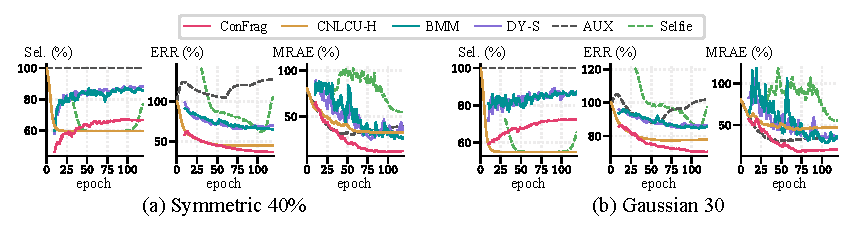
\includegraphics[width=\textwidth]{imgs/selerr_comparison_neurips.pdf}}
\vskip -0.1in
\caption{\textbf{Selection/ERR/MRAE comparison}
between ConFrag and strong baselines of CNLCU-H, BMM, DY-S, AUX and Selfie on IMDB-Clean-B. We exclude the performance during the warm-up. %phase.
%Note that the selection of CNLCU-H and Sigua are identical, as they base their Selection rate on noise rate information.
%In addition to FragSel, we include the two most strongly performing sample selection 
%baselines, Sigua~\citep{han20sigua} and CNLCU-H~\citep{xia22}. The experiments are based on IMDB-Clean-B~\citep{rothe18imdb}.
% TODO show MRAE on the right y-axis and show how they differ.
}
\label{fig:hse}
\end{center}
\vskip -0.25in
\end{figure*}

\subsection{Evaluation Metrics}\label{subsec:evaluation_metrics}
We mainly report the Mean Relative Absolute Error (MRAE) following prior works. 
The MRAE is computed as $(e/\rho)-1$, where $e$ is the model's Mean Absolute Error (MAE) performance under varying conditions (noise type, severity) and $\rho$ is the noise-free model's MAE. % for the corresponding dataset.
We express MRAEs in percentage for better comprehensibility. 
The traditional MAE values are also reported in Appendix~\ref{subsec:mae}.
In addition, we report the Selection rate (a.k.a prevalence), which is a metric often seen in noisy labeled classification to quantify the coverage of the total dataset, $|\mathcal{S}|/|\mathcal{D}|$ where $\mathcal{S}$ and $\mathcal{D}$ are the selected and total set, respectively. %The precision/purity is usually paired with the Selection rate in noisy labeled classification. However, to account for the fluctuating degrees of noise in regression, we propose the ERR metric instead. 

\textbf{Error Residual Ratio}. 
To better assess selection and refurbishment approaches, we introduce a new metric termed Error Residual Ratio (ERR).
%We propose a simple evaluation measure for selection and refurbishment approaches in noisy label regression tasks. 
Unlike classification, noisy labels in regression can show the diverse severity of the noise present in each label $y$ (\ie various degrees of deviation from the ground truth $y^\text{gt}$). 
This cannot be addressed when using conventional metrics, which are primarily designed for classification and tend to treat all instances of noise as equally severe. 
Our proposed ERR considers the varying severity of noise and is defined as
\begin{gather}\label{eq:ERR}
    % \text{selection} &= \frac{|\text{TP}| + |\text{FP}|}{|\mathcal{D}|} \quad \quad \text{error reduction} = 1 - \frac{\sum_s^{|S|} |\tilde{y}^c_s - y^c_s|}{ \sum_d^{|\mathcal{D}|} |\tilde{y}^c_d - y^c_d|}\\
    % \text{selection} &= \frac{|\mathcal{S}|}{|\mathcal{D}|} \quad \quad \text{error reduction} = 1 - \frac{\sum_s^{|S|} |\tilde{y}^c_s - y^c_s|}{ \sum_d^{|\mathcal{D}|} |\tilde{y}^c_d - y^c_d|}\\
    % \text{Error Residual Ratio (ERR)} = \frac{\mfrac{\sum_s^{|S|} |\tilde{y}^c_s - y^c_s|}{|S|}}{ \mfrac{\sum_d^{|\mathcal{D}|} |\tilde{y}^c_d - y^c_d|}{|D|}}\\
    % XXX below if final chosen one.
   \text{ERR} = \frac{1/|\mathcal{C}|\sum_c^{|\mathcal{C}|} |y_c - y^\text{gt}_c|}{1/|\mathcal{D}|\sum_d^{|\mathcal{D}|} |{y}^\text{ }_d - y^\text{gt}_d|},
    % \text{Error Residual Ratio (ERR)} = \mfrac{1}{|\mathcal{S}|}\sum_s^{|S|} |\tilde{y}^c_s - y^c_s|/\mfrac{1}{|\mathcal{D}|}\sum_d^{|\mathcal{D}|} |\tilde{y}^c_d - y^c_d|
    % \text{Error Residual Ratio (ERR)} = \frac{\sum_s^{|S|} |\tilde{y}^c_s - y^c_s|/|S|}{ \sum_d^{|\mathcal{D}|} |\tilde{y}^c_d - y^c_d|/|D|}
\end{gather}
where $\mathcal{C}$ is a set of cleaned (selected or refurbished) samples. 
The numerator is the average cleaned error that serves as an indicator of the precision of the cleaned data, while the denominator is the average dataset error that normalizes it for standardized assessment.
The ERR, along with the selection rate and regression metrics (\eg MSE, MRAE), provides a deeper insight into the model performance.
% Ideally, a method with a high selection rate coupled with low ERR and regression metric scores, can be deemed as closer to the upper bound.
Ideally, a method with a high selection rate coupled with low ERR and regression error can be deemed as closer to the upper bound.
% where while simultaneously distinguishing the assessment of, collectively denoted as cleaned , from the inherent capability of the regression model in mitigating the impact of noise.

% \subsection{Evaluation Metrics}\label{subsec:evaluation_metrics}
% We mainly report the Mean Relative Absolute Error (MRAE) for all experiments. 
% We also report the Selection rate and the Error Residual Ratio (ERR) for selection/refurbish-based approaches.
% The MRAE is computed as $(e/\rho)-1$, where $e$ is the model's MAE performance under varying conditions (data, noise type, severity) and $\rho$ is the fixed noise-free model's MAE for the corresponding dataset.
% Note that we express MRAEs in percentage for better comprehensibility.
% Furthermore, the traditional MAE values are also reported in Appendix~\ref{subsec:mae}.
% The Selection rate (a.k.a prevalence) is a metric often seen in noisy classification to quantify the coverage of the total dataset, $|\mathcal{S}|/|\mathcal{D}|$ where $\mathcal{S}$ is the selected set, $\mathcal{D}$ is the total dataset.
% % XXX % Notably, continuous labels can easily be slightly wrong, but still be useful for the task at hand. Therefore Selection amount for coverage needs to be used instead of recall.
% % \subsubsection{HSE: Harmonic Selection Error Reduction Score}\label{subsubsec:HSE}
% % % Since noisy label regression evaluation relies heavily on MAE/MRAE scores; we propose our novel HSE metric to evaluate the outcome from a different dimension.
% % % Due to the absence of an appropriate regression label noise evaluation measure for the selected/refurbished samples,
% % % We propose a regression label noise evaluation measure for the selected/refurbished samples. 
% % We propose a regression label noise evaluation measure for selection and refurbishment approaches. 
% % The key aspect to consider in the metric's design is the varying severity of the noise in the regression labels. 
% % That is, Each label noise ($\tilde{y}^c$) can have differing distance amounts from the ground truth ($y^c$). 
% % However, existing metrics often seen in classification tasks treat them as equals, resulting in a vastly imprecise evaluation.
% % Hence, we design a metric that isolates the evaluation of the selected/refurbished samples from the regression model/algorithm's innate ability to mitigate the effects of the noise while accounting for the reduced error amount and selection rate for coverage (a.k.a prevalence). 
% % This is formulated as the harmonic mean of the two criteria to evaluate the selected set, $\mathcal{S}$.
% % % XXX % Notably, continuous labels can easily be slightly wrong, but still be useful for the task at hand. Therefore Selection amount for coverage needs to be used instead of recall.
% % % Also, training a regression task with higher amount of dataset error gives worse performance than smaller amount of dataset error.
% % \begin{align}\label{eq:HSE}
% %     % \text{selection} &= \frac{|\text{TP}| + |\text{FP}|}{|\mathcal{D}|} \quad \quad \text{error reduction} = 1 - \frac{\sum_s^{|S|} |\tilde{y}^c_s - y^c_s|}{ \sum_d^{|\mathcal{D}|} |\tilde{y}^c_d - y^c_d|}\\
% %     % \text{selection} &= \frac{|\mathcal{S}|}{|\mathcal{D}|} \quad \quad \text{error reduction} = 1 - \frac{\sum_s^{|S|} |\tilde{y}^c_s - y^c_s|}{ \sum_d^{|\mathcal{D}|} |\tilde{y}^c_d - y^c_d|}\\
% %     \text{selection} &= \frac{|\mathcal{S}|}{|\mathcal{D}|} \quad \quad \text{error residual ratio} = \frac{\mfrac{\sum_s^{|S|} |\tilde{y}^c_s - y^c_s|}{|S|}}{ \mfrac{\sum_d^{|\mathcal{D}|} |\tilde{y}^c_d - y^c_d|}{|D|}}\\
% %     % \alpha_f &= \left[ \left(p(y=y^d_{fn} | X; \theta_{fn, fn^+}) > p(y=y^d_{fn^+}|X;\theta_{fn,fn^+})\right) \land y^d_{fn} \in \{ y^d_{fL}, y^d_{fR} \} \right]
% %     % \text{HSE} &= 2 \cdot \frac{\text{selection} \cdot \text{error reduction}}{\text{selection} + \text{error reduction}}
% %     \text{HSE} &= \frac{2}{\text{selection}^{-1} + \text{error reduction}^{-1}}
% % \end{align}
% % where $\mathcal{D}$ is the total data set. 
% % Analyzing HSE alongside the regression metrics (\eg MSE, MRAE), HSE can offer a different insight into the upper bound of the model performance and the direction for improvment.
% % Ideally, a method performing well in \textit{both} regression metrics and HSE can be deemed more complete.
% % We propose a simple evaluation measure for selection and refurbishment approaches in noisy label regression tasks. 
% % A key characteristic of noisy regression labels we must consider is the varying severity of the noise.
% % That is, each label noise ($y$) can exhibit varying degrees of deviation from the ground truth ($y^\text{gt}$). 
% % This nuanced aspect is often overlooked by existing metrics, such as precision and recall, which are traditionally employed in classification tasks. 
% % When these classification-centric metrics are adapted for use in regression scenarios, they tend to treat all noise instances as equally severe. 
% % Consequently, this misalignment results in imprecise evaluations that fail to account for the diverse nature of noise severity in regression problems.
% % ERR is crafted to consider the varying severity of noise while disentangling the assessment of selected/refurbished samples from the inherent capacity of the regression model/algorithm to mitigate the impact of noise.
% % This metric is crafted to disentangle the assessment of selected/refurbished samples from the inherent capacity of the regression model/algorithm to mitigate the impact of noise.
% % A key consideration in designing this metric is the variable severity of noise present in the regression labels. 
% % That is, each label noise ($y$) can exhibit varying degrees of deviation from the ground truth ($y^\text{gt}$). 
% % This nuanced aspect is often overlooked by existing metrics, such as precision and recall, which are traditionally employed in classification tasks. 
% % When these classification-centric metrics are adapted for use in regression scenarios, they tend to treat all noise instances as equally severe. 
% % Consequently, this misalignment results in imprecise evaluations that fail to account for the diverse nature of noise severity in regression problems.
% % Hence, we design a metric that isolates the evaluation of the selected/refurbished samples from the regression model/algorithm's innate ability to mitigate the effects of the noise.

% \textbf{ERR: Error Residual Ratio}.
% We propose a simple evaluation measure for selection and refurbishment approaches in noisy label regression tasks. 
% A crucial characteristic of noisy regression labels is the variable severity of the noise present in each label ($y$), which can exhibit various degrees of deviation from the ground truth ($y^\text{gt}$). 
% This cannot be addressed when using conventional metrics like precision and recall, since they tend to treat all instances of noise as equally severe. 
% % Consequently, this misalignment leads to imprecise evaluations that do not adequately account for the diverse spectrum of noise severity encountered in regression problems.
% Our proposed Evaluation Metric for Regression Noise (ERR) considers the varying severity of noise while concurrently separating the assessment of selected or refurbished samples from the inherent capability of the regression model in mitigating the impact of noise.
% The metric is defined as
% \begin{align}\label{eq:ERR}
%     % \text{selection} &= \frac{|\text{TP}| + |\text{FP}|}{|\mathcal{D}|} \quad \quad \text{error reduction} = 1 - \frac{\sum_s^{|S|} |\tilde{y}^c_s - y^c_s|}{ \sum_d^{|\mathcal{D}|} |\tilde{y}^c_d - y^c_d|}\\
%     % \text{selection} &= \frac{|\mathcal{S}|}{|\mathcal{D}|} \quad \quad \text{error reduction} = 1 - \frac{\sum_s^{|S|} |\tilde{y}^c_s - y^c_s|}{ \sum_d^{|\mathcal{D}|} |\tilde{y}^c_d - y^c_d|}\\
%     % \text{Error Residual Ratio (ERR)} = \frac{\mfrac{\sum_s^{|S|} |\tilde{y}^c_s - y^c_s|}{|S|}}{ \mfrac{\sum_d^{|\mathcal{D}|} |\tilde{y}^c_d - y^c_d|}{|D|}}\\
%     % XXX below if final chosen one.
%    \text{Error Residual Ratio (ERR)} = \frac{\mfrac{1}{|\mathcal{S}|}\sum_s^{|S|} |y_s - y^\text{gt}_s|}{\mfrac{1}{|\mathcal{D}|}\sum_d^{|\mathcal{D}|} |{y}^\text{ }_d - y^\text{gt}_d|}
%     % \text{Error Residual Ratio (ERR)} = \mfrac{1}{|\mathcal{S}|}\sum_s^{|S|} |\tilde{y}^c_s - y^c_s|/\mfrac{1}{|\mathcal{D}|}\sum_d^{|\mathcal{D}|} |\tilde{y}^c_d - y^c_d|
%     % \text{Error Residual Ratio (ERR)} = \frac{\sum_s^{|S|} |\tilde{y}^c_s - y^c_s|/|S|}{ \sum_d^{|\mathcal{D}|} |\tilde{y}^c_d - y^c_d|/|D|}
% \end{align}
% % where $\mathcal{D}$ is the total data set. 
% Analyzing ERR along with the selection rate and regression metrics (\eg MSE, MRAE) provides a deeper insight into the model performance. %, offering valuable insights into potential avenues for enhancement. %and hints at the directions for further improvements.
% Ideally, a method with a high selection rate, coupled with low ERR and favorable regression metric scores, can be deemed as closer to the upper bound.
% % Ideally, a method performing well in \textit{both} regression metrics and HSE can be deemed more complete.

% TODO Additional points to consider... 
% \begin{itemize}
%     \item There are mainly sample selection, refurbishment, and regularization methods in noisy labels. HSE can offer a deeper insight on refurbishment and selection methods.
%     \item Similar to the F1 score, HSE offers another perspective other than simple MAE, offering deeper insight into WHY the model performs well. 
%     Such as, the model could perform well with a small selection of samples and a high error reduction 
%     or a large selection of samples and a small error reduction. This is something MAE cannot offer in its scores alone.
%     Type I or Type II errors cannot be immediately considered in regression. 
%     \item consider the diversity score also so that the diversity of the selected samples can be considered from a label and embedding perspective.
%     % \item AUC curve can also be considered. For the scenarios with Imbalance and robust applications.
%     % \item Classification noisy label also can use as a cost-considered metric... But this is difficult to generalize at the moment!
%     \item HSE follows a similar pattern as that of MAE, and HSE does not require training...! (already checked)
% \end{itemize}
% F1 preferred over accuracy when data is imbalanced.

% The key aspect of SE is to measure the selection's or refurbished data's effectiveness in reducing the noise's severity and selection amount.
% The desiderata to account for continuous label noise metric is as follows: 1. Severity of the noise,
% 2. Selection amount.

\subsection{Results and Discussion}\label{sec:discussion}
\textbf{Overall performance.}
Table~\ref{tab:main_mrae} compares the MRAE values to 
the noise-free trained model between ConFrag and the baselines.
We evaluate six types of noise: four symmetric and two random Gaussian noises. 
ConFrag and Co-ConFrag achieve the strongest performance in all experiments compared to the fourteen baselines.
Notably, Co-ConFrag mixes co-teaching during the regression learning phase by assuming that $\mathcal{S}$ still contains 25\% noise.
The results on UTKFace-B dataset can be found in Appendix~\ref{subsec:utkface}.
% Particularly, it performs better than the small-loss based approaches (CNLCU, Sigua, Selfie), which assumes the noise rates are known in advance.
% XXX main table explanation and analysis. Why some branches do better than the other. Why some baselines fail.

\textbf{Selection/ERR/MRAE comparison.} 
% In Fig.~\ref{fig:hse}, we compare the Selection rate and ERR of FragSel and five
%  selection/refurbishment baselines (CNLCU-H, BMM, DY-S, Selfie, AUX) on IMDB-Clean-B dataset. 
% An optimal model would have a high Selection rate and a low ERR.
% Note that it should be dataset-dependent as to which ERR or Selection rate is more important. 
% However, in our experiments, we observe that ERR significantly influences the final performance.
% Notably, FragSel always arrives at the lowest ERR with above-average Selection rates, hinting at a possible future direction for improvement involving refurbishment.
% Fig.~\ref{fig:hse} compares the selection rate, ERR, and MRAE for FragSel and five selection and refurbishment baselines of CNLCU-H, BMM, DY-S, AUX, Selfie on IMDB-Clean-B.
Fig.~\ref{fig:hse} compares ConFrag to five selection and refurbishment baselines of CNLCU-H, BMM, DY-S, AUX, Selfie on IMDB-Clean-B using the selection rate, ERR, and MRAE.
Ideally, a model should attain a high selection rate and a low ERR.
% It is worth noting that the relative importance of ERR and selection rate may vary depending on the dataset and the task at hand. 
It is worth noting that the relative importance of ERR and selection rate may vary depending on the dataset and the task. 
% In our experiments, we observe that ERR significantly influences the final performance of the models.
% Notably, FragSel achieves the lowest ERR while maintaining above-average selection rates. 
ConFrag achieves the lowest ERR while maintaining above-average selection rates, resulting in the best MRAE.
% This hints at a potential future direction for improvement, particularly in the area of refurbishment.
% We observe a relatively gradual increase in the ERR when the noise rate is low.
% One of the main reasons for this is that both Sigua and CNLCU-H assume a known noise rate in advance,
% allowing random selection to achieve a selection rate of 0.80 in 20\% noise, for instance.
% Nevertheless, FragSel slightly outperforms the two baselines at 20\% and noticeably performs better in all other noise levels. 
% Appendix~\ref{subsec:ERR} includes \textcolor{magenta}{more experiments and analysis}.%all noise types with more baseline comparison results.
Appendix~\ref{subsec:ERR} includes comparison results for all noise types with more baselines.

% \begin{figure}[t]
% \begin{center}
% \centerline{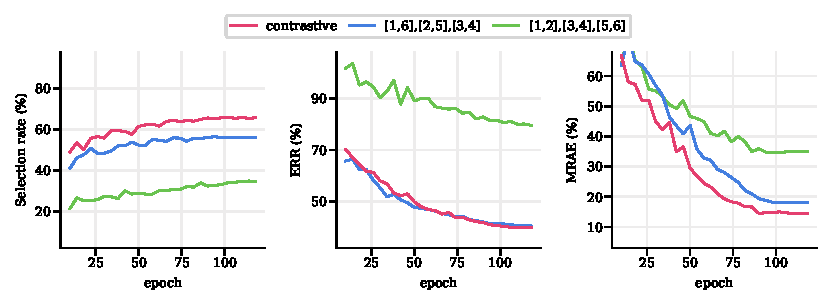
\includegraphics[width=0.8\textwidth]{imgs/fragmentation_analysis_wide_main.pdf}}
% \vskip -0.1in
% \caption{
% % \textbf{Contrasting Fragment combination analysis} compares contrastive pairings ([1,4], [2,5], [3,6]) and two versions of all-fragments ([1,2,3,4,5,6]) on IMDB-Clean-B with 40\% symmetric noise.
% % Contrastive pairings use ResNet-18, while all-fragments use a ResNet-34 backbone.
% % }
% \textbf{Fragment pairing analysis} comparing contrastive pairings ($[1,4], [2,5], [3,6]$) to other pairing methods ($[1,2],[3,4],[5,6]$ and $[1,6],[2,5],[3,4]$) on IMDB-Clean-B with 40\% symmetric noise.
% % All-fragments use a ResNet-34, while other pairing methods use ResNet-18 backbones.
% }
% \vskip -0.4in
% \label{fig:fragment_pairing_main}
% \end{center}
% \end{figure}



\textbf{Fragment pairing.}
Fig.~\ref{fig:discussion_main}(a) compares contrastive pairing to alternative pairings 
%($[1,2],[3,4],[5,6]$ and $[1,6],[2,5],[3,4]$) 
using MRAE as a metric. % selection rate, ERR, and MRAE as metrics.
The contrastive fragment pairing demonstrates superior performance to other pairing methods.
Notably, the performance is poorest when both the average and minimum distance between fragments are smallest ($[1,2], [3,4]$ when $F=4$, $[1,2],[3,4],[5,6]$ when $F=6$).
While the pairings of $[1,4], [2,3]$ and $[1,6],[2,5],[3,4]$ have the same average distance between fragments as the contrastive pairings, their minimum distances between fragments are smaller, resulting in poorer performances than contrastive pairings.
This result shows the effectiveness of contrastive fragment pairing for selecting clean samples.
See Appendix~\ref{subsec:contrast_combination} for more details. %with other metrics and feature visualization.

\textbf{Fragment number.}
ConFrag introduces a hyperparameter $F$, the number of fragments.
While we simply set $F=4$ for all experiments, we conduct analysis on the effect of using different $F$, as shown in Fig.~\ref{fig:discussion_main}(b).
On SHIFT15M-B dataset, the performance is relatively stable across different fragment numbers.
On IMDB-Clean-B, a small declining trend in performance is observed as the number of fragments increases.
This decrease is likely attributed to a finer division of the training data among feature extractors, ultimately leading to overfitting and reduced generalization capabilities.
% Thus the optimal number of fragments depends on the task and dataset.
Appendix~\ref{subsec:fragment_numbers} provides further analysis of the fragment number.
% \textbf{[Deprecated]}
% The optimal number of fragmentations can be determined by leveraging ERR and selection rate as a proxy for the MRAE of the downstream task. 
% Specifically, following previous studies using mixture models~\cite{dai2024} we train encoders by searching a small range of fragment numbers. 
% For each fragment number, we calculate the harmonic mean of ($1-$ ERR) and the selection rate of FragSel. 
% Fig.~\ref{fig:fragnum_analysis} illustrates how this harmonic mean accurately correlates to the best MRAE in the downstream task. 
% % Notably, this approach does not necessitate training the downstream task. %it can be efficiently computed through parallelization. 
% Importantly, this approach enables us to bypass the training of the downstream task.
% % In essence, it can be treated as any other hyperparameter in our optimization process. 
% Further analysis of the fragment number is in Appendix~\ref{subsec:fragment_numbers}.
% % A better direction for future research would be to consider the dataset's intracacies~\citep{ethayarajh22icml}, which is beginning to to studied, and could be useful in approximating the optimal number of fragments.
% Another direction would involve the examination of the dataset's intricacies such as \citep{ethayarajh22icml}, %, have begun to explore.
% which can aid the trainless estimation of the number of fragments.

% The choice of an optimal \textit{total} number of fragments is contingent upon the dataset's inherent difficulty, an aspect that is garnering increasing attention in the research community~\citep{ethayarajh22icml}. 
% In this study, we adopt the simplest configuration by setting the total number of fragments to four, and yet, we consistently observe significant improvements in performance across all our experiments.
% Following selection, we can discard the ``noise” parameters, retaining only ``regr” parameters for regression.
% In all experiments, we use a fixed model size for regression training (except co-train, CNLCU).
% \textbf{Discretized Baselines.} Since we employ the cross entropy loss to train our feature extractor, for fairness we also study the discretized version of several strong baselines in Table~\ref{tab:discrete}.
% The class ids are obtained through the discretization we used for FragSel, 
% \textbf{Ablation Analysis.} In Appendix~\ref{subsec:ablation}, we conduct an analysis of FragSel's design choices and its compatibility with other techniques. 
% Notably, we observed significant performance improvements, particularly when employing neighborhood jittering with vanilla cross entropy during feature extractor training. 
% Moreover, both self-agreement ($\alpha_f^\text{self}$) and neighbor-agreement ($\alpha_f^\text{ngb}$) proved to be valuable in obtaining cleaner samples. 
% Additionally, we found that other noisy label techniques, such as C-Mixup and Co-teaching, consistently led to substantial performance enhancements. 
% However, it is worth noting that the regularization techniquea such as symmetric cross-entropy (SCE) did not yield substantial benefits.

\begin{figure}[t]
    \begin{center}
    %\vskip -0.1in
    \centerline{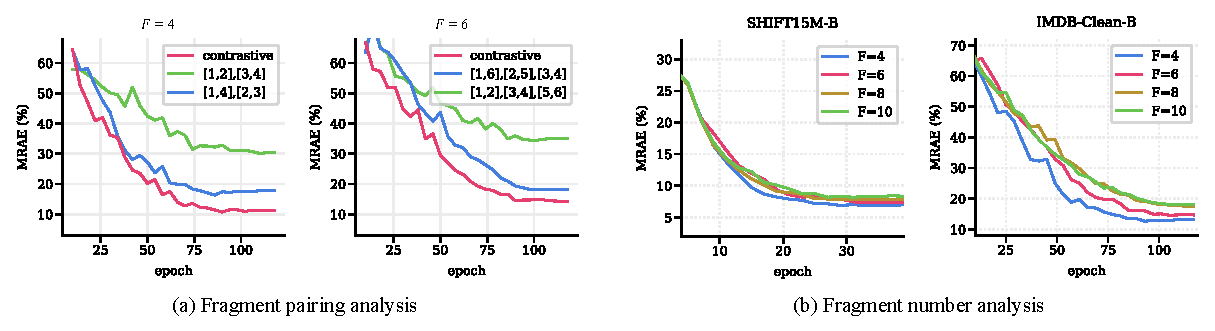
\includegraphics[width=0.95\textwidth]{imgs/discussion_figure_neurips_v2.pdf}}
    \vskip -0.1in
    \caption{
    % \textbf{Contrasting Fragment combination analysis} compares contrastive pairings ([1,4], [2,5], [3,6]) and two versions of all-fragments ([1,2,3,4,5,6]) on IMDB-Clean-B with 40\% symmetric noise.
    % Contrastive pairings use ResNet-18, while all-fragments use a ResNet-34 backbone.
    % }
    \textbf{Analysis} with 40\% symmetric noise. (a) Comparison between the proposed contrastive pairing  and other pairings on IMDB-Clean-B.
    (b) Comparison between fragment numbers on SHIFT15M-B and IMDB-Clean-B.
    }
    \vskip -0.3in
    \label{fig:discussion_main}
    \end{center}
    \end{figure}
    

\begin{table}[t]
    \hspace{-2.5pt}
    \begin{minipage}{.55\textwidth}
        \centering
        \begin{small}
        \setlength{\tabcolsep}{4.2pt}
        \caption{\textbf{Ablation of Mixture of Neighboring Fragments.}
        % The values are mean relative absolute error (MRAE) to the noise-free model on the IMDB-Clean-B dataset, and lower values indicate better performances.
        MRAE on the IMDB-Clean-B dataset (lower is better).
        % The results are the mean of three random seed experiments.
        }
        \label{tab:ablation_mnf}
        \begin{tabular}{cccccc}
            \toprule
            %\multicolumn{3}{c}{ablation}&\multicolumn{3}{c}{IMDB-Clean-B}
            %\\\cmidrule(lr){1-3} \cmidrule(lr){4-6}
            & & & \multicolumn{1}{c}{symmetric}    &\multicolumn{2}{c}{Gaussian} \\
            %\midrule
            $\alpha_f^\text{self}$ & $\alpha_f^\text{ngb}$ & $\mathcal{S}$ & 40 & 30 & 50\\
            \midrule
            % \specialrule{0.7pt}{1pt}{1pt}
            \checkmark &            & $\mathcal{S}^p\cup \mathcal{S}^r$  & 16.97 & 17.53 & 38.18 \\
                    & \checkmark & $\mathcal{S}^p\cup \mathcal{S}^r$  & 22.22 & 22.77 & 46.36 \\
            % \checkmark & \checkmark & $\mathcal{S}^p$                    & 23.13 & 22.54 & 46.65 \\ % no jit
            \checkmark & \checkmark & $\mathcal{S}^p$                    & 14.18 & 15.84 & 33.07 \\
            % \checkmark & \checkmark & $\mathcal{S}^r$                    & 21.90 & 22.02 & 45.03 \\ % no jit
            \checkmark & \checkmark & $\mathcal{S}^r$                    & 14.06 & 16.94 & 39.85 \\
            \checkmark & \checkmark & $\mathcal{S}^p\cap \mathcal{S}^r$  & 13.08 & 16.18 & 34.23 \\
            \checkmark & \checkmark & $\mathcal{S}^p\cup \mathcal{S}^r$  & 12.64 & 15.70 & 33.36 \\

            \bottomrule
        \end{tabular}
        \end{small}
    \end{minipage}
    \hspace{5pt}
    \begin{minipage}{.45\textwidth}
        \vspace{-3.7pt}
        \caption{\textbf{Parameter size comparison}. regression: parameters for regression, noise: parameters to mitigate noisy labels, ``others": SPR, CDR, D2L, C-Mixup, Sigua, Selfie, BMM, DY-S, Superloss.}
        \label{tab:param_compare}
        \centering
        \begin{footnotesize}
        \setlength{\tabcolsep}{3.0pt}
        \begin{tabular}{lccc}
            \toprule
            & regression & noise & total  \\
            \midrule
            RDI & 23.9M & 47.8M & 47.8M \\
            \specialrule{0.1pt}{1pt}{1pt}
            CNLCU & 47.8M & 47.8M & 47.8M \\
            \specialrule{0.1pt}{1pt}{1pt}
            ``others" & 23.9M & 23.9M & 23.9M \\
            \specialrule{0.1pt}{1pt}{1pt}
            ConFrag & 23.9M & 22.8M & 46.7M \\
            \bottomrule
        \end{tabular}
        \end{footnotesize}
    \end{minipage}
\end{table}

\begin{comment}
\begin{table}[t]
    \centering
    \begin{small}
    \setlength{\tabcolsep}{4.2pt}
    \caption{\textbf{Ablation of Mixture of Neighboring Fragments.}
    The values are mean relative absolute error (MRAE) to the noise-free model on the IMDB-Clean-B dataset, and lower values indicate better performances.
    The results are the mean of three random seed experiments.
    }
    \label{tab:ablation_mnf}
    \begin{tabular}{cccccc}
        \toprule
        \multicolumn{3}{c}{ablation}&\multicolumn{3}{c}{IMDB-Clean-B}
        \\\cmidrule(lr){1-3} \cmidrule(lr){4-6}
        & & & \multicolumn{1}{c}{symmetric}    &\multicolumn{2}{c}{Gaussian} \\
        %\midrule
        $\alpha_f^\text{self}$ & $\alpha_f^\text{ngb}$ & $\mathcal{S}$ & 40 & 30 & 50\\
        \midrule
        % \specialrule{0.7pt}{1pt}{1pt}
        \checkmark &            & $\mathcal{S}^p\cup \mathcal{S}^r$  & 16.97 & 17.53 & 38.18 \\
                & \checkmark & $\mathcal{S}^p\cup \mathcal{S}^r$  & 22.22 & 22.77 & 46.36 \\
        % \checkmark & \checkmark & $\mathcal{S}^p$                    & 23.13 & 22.54 & 46.65 \\ % no jit
        \checkmark & \checkmark & $\mathcal{S}^p$                    & 14.18 & 15.84 & 33.07 \\
        % \checkmark & \checkmark & $\mathcal{S}^r$                    & 21.90 & 22.02 & 45.03 \\ % no jit
        \checkmark & \checkmark & $\mathcal{S}^r$                    & 14.06 & 16.94 & 39.85 \\
        \checkmark & \checkmark & $\mathcal{S}^p\cap \mathcal{S}^r$  & 13.08 & 16.18 & 34.23 \\
        \checkmark & \checkmark & $\mathcal{S}^p\cup \mathcal{S}^r$  & 12.64 & 15.70 & 33.36 \\

        \bottomrule
    \end{tabular}
    \end{small}
\end{table}

\begin{table}[t]
    \caption{\textbf{Parameter size comparison}. regression: parameters for regression, noise: parameters to mitigate noisy labels, ``others": SPR, CDR, D2L, C-Mixup, Sigua, Selfie, BMM, DY-S, Superloss.}
    \label{tab:param_compare}
    \centering
    \begin{footnotesize}
    \setlength{\tabcolsep}{3.0pt}
    \begin{tabular}{lccc}
        \toprule
          & regression & noise & total  \\
        \midrule
        RDI & 23.9M & 47.8M & 47.8M \\
        \specialrule{0.1pt}{1pt}{1pt}
        CNLCU & 47.8M & 47.8M & 47.8M \\
        \specialrule{0.1pt}{1pt}{1pt}
        ``others" & 23.9M & 23.9M & 23.9M \\
        \specialrule{0.1pt}{1pt}{1pt}
        ConFrag & 23.9M & 22.8M & 46.7M \\
        \bottomrule
    \end{tabular}
    \end{footnotesize}
\end{table}
\end{comment}

\textbf{Ablation analysis on mixture of neighboring fragments.}
In Table~\ref{tab:ablation_mnf}, we conduct an ablation analysis of the Mixture of neighboring fragments (\S~\ref{subsec:mixture_of_contrasing_fragments}).
When evaluating neighborhood agreement based solely on either the agreement of the current fragment ($\alpha_f^\text{self}$) or the neighboring fragment's agreement ($\alpha_f^\text{ngb}$),
the ablation reveals that relying on the current fragment's agreement alone ($\alpha_f^\text{self}$) exhibited relatively stronger performance.
Nevertheless, this approach still fell short of achieving a satisfactory level compared to considering both agreements, as defined in Eq.~\ref{eq:na_final}.

Next, as we consider sample selection based on two variants of agreements, the \textit{predictive} one utilizing the feature extractor's binary classifier and the \textit{representational} one using $K$-nearest neighbors on the learned feature space
(referred to as the selected sample sets $\mathcal{S}^p$ and $\mathcal{S}^r$ respectively), we conduct an ablation study on these selected sample sets.
This involves evaluating the results when determining the final selected sample set ($\mathcal{S}$) either individually, at the intersection, or at the union of $\mathcal{S}^p$ and $\mathcal{S}^r$.
Overall, in line with ConFrag, the union of sets ($\mathcal{S}^p \cup \mathcal{S}^r$) proves to be the most effective strategy.

\textbf{Parameter size comparison.}
Table~\ref{tab:param_compare} compares the number of parameters of ConFrag and baselines on the ResNet-based age prediction datasets. %, AFAD-B and IMDB-Clean-B.
A thorough description of the ConFrag architecture is in Appendix~\ref{subsec:training_details}.
It is worth noting that each of the ConFrag's feature extractors for noise mitigation employs a much fewer number of parameters than the downstream regression task (\eg 48\% in age prediction datasets). %IMDB-Clean-B and AFAD-B).
The total number of parameters of each method varies, as some share parameters for regression as well as noise mitigation while others, such as ConFrag, do not.
Nevertheless, ConFrag uses fewer total parameters than CNLCU-H and RDI.

% \textbf{Appendix.} We supplement the limitation (\ref{sec:limitations}), 
%the parameter size comparison (\ref{subsec:param_size}), 
% fragment number analysis~\ref{subsec:fragment_numbers}, \textcolor{magenta}{hyperparameter analysis~\ref{subsec:hyperparameter}}, performances of the discretized version of the baselines~\ref{subsec:discrete_baselines}, 
% ablation study~\ref{subsec:ablation}, variance analysis~\ref{subsec:variance}, disruptive versus anomalous noise analysis~\ref{subsec:disruptive_anomaly_noise}, \textcolor{magenta}{FragSel pseudo code~\ref{alg:fragmented_selection}}.
% hyperparameter setting (\ref{subsec:hyperparameter}), analysis on closed-set versus open-set noise (\ref{subsec:disruptive_anomaly_noise}), variance with respect to random seed (\ref{subsec:variance}),
% hyperparameter setting (\ref{subsec:hyperparameter}), more ablation studies (\ref{subsec:ablation}), performance of the discretized version of the baselines (\ref{subsec:discrete_baselines}), and variance with respect to random seed (\ref{subsec:variance}).

\section{Conclusion}\label{sec:conclusion}
\vskip -0.05in
To address the problem of noisy labeled regression, we introduce the Contrastive Fragmentation framework (ConFrag). 
The framework partitions the label space and identifies the most contrasting pairs of fragments, thereby training a mixture of feature extractors over contrastive fragment pairs.
This mixture is leveraged for clean selection based on neighborhood agreements.
% contrasting pairs of fragments to train a mixture of contrasting fragments for clean selection based on neighbor agreements.
Extensive experiments on six curated datasets on three domains with different levels of symmetric and Gaussian noise demonstrate that our framework performs superior selection and ultimately leads to a better regression performance than fourteen state-of-the-art models.
Given its foundation in the Mixture of Experts model, the parameter size of ConFrag linearly grows with an increase in the number of fragments. 
We acknowledge this as a potential avenue for future research.
% FragSel exhibits linear growth in parameter size with an increase in the number of fragments. 
% We acknowledge this as a potential avenue for future research and development.

\section*{Acknowledgement}
We express our gratitude to the members of the Vision and Learning Lab at Seoul National University for their valuable feedback on the manuscript.
In particular, we would like to acknowledge Jaekyeom Kim, Soochan Lee, Jinseo Jeong, Wonkwang Lee, and Sehun Lee.
This work was supported by 
LG AI Research,
Institute of Information \& Communications Technology Planning \& Evaluation (IITP) grant funded by the Korea government (MSIT) (No.~RS-2019-II191082, SW StarLab), % 스타랩
Institute of Information \& communications Technology Planning \& Evaluation (IITP) grant funded by the Korea government (MSIT) (No.~RS-2022-II220156, Fundamental research on continual meta-learning for quality enhancement of casual videos and their 3D metaverse transformation), % 사람중심AI 
the National Research Foundation of Korea (NRF) grant funded by the Korea government (MSIT) (No.~2023R1A2C2005573), % 중견
and Institute of Information \& communications Technology Planning \& Evaluation (IITP) grant funded by the Korea government (MSIT) (No.~RS-2021-II211343, Artificial Intelligence Graduate School Program (Seoul National University)).  % AI대학원
Gunhee Kim is the corresponding author.
\bibliography{ref}
\bibliographystyle{plainnat}

%%%%%%%%%%%%%%%%%%%%%%%%%%%%%%%%%%%%%%%%%%%%%%%%%%%%%%%%%%%%



%%%%%%%%%%%%%%%%%%%%%%%%%%%%%%%%%%%%%%%%%%%%%%%%%%%%%%%%%%%%

\newpage
\appendix

\section{Appendix: Table of Contents}


% The $\mathtt{\backslash onecolumn}$ command above can be kept in place if you prefer a one-column appendix, or can be removed if you prefer a two-column appendix.  Apart from this possible change, the style (font size, spacing, margins, page numbering, etc.) should be kept the same as the main body.
The Appendix enlists the following additional materials. %which may shed further insights:
\begin{enumerate}[label=\Roman*.]
    \item Limitations. \S~\ref{sec:limitations}
    \item Broader Impacts. \S~\ref{sec:broader_impacts}
    \item Theory of ConFrag. \S~\ref{sec:theory}
        \begin{enumerate}[label=\roman*.]
            \item Classification versus Regression for Feature Learning~\ref{subsec:classification_vs_regression}
            \item Fragmentation and Neighborhood Jittering~\ref{subsec:fragmentation_and_neighborhood_jittering}
            \item Prediction Depth Analysis~\ref{subsec:prediction_depth_analysis}
        \end{enumerate}
    \item Extended Related Work. \S~\ref{subsec:related_work}
        \begin{enumerate}[label=\roman*.]
            \item Continuously Ordered Correlation of Labels and Features~\ref{subsec:continuity_related_works}
            \item Noisy Label in Object Detection~\ref{subsec:object_detection_related_works}
            \item Transition Matrix based Methods~\ref{subsec:transition_matrix_related_works}
            \item Combination with Contrastive Learning~\ref{subsec:contrastive_learning_related_worls}
        \end{enumerate}
    \item Experiment Details. \S~\ref{sec:exp_details}
        \begin{enumerate}[label=\roman*.]
            \item Dataset Curation Details~\ref{subsec:dataset_curation}
            \item Baseline Details~\ref{subsec:baselines}
            \item ConFrag Training Details~\ref{subsec:training_details}
            \item Random Gaussian Noise~\ref{subsec:random_gaussian}
            \item Computation Resource~\ref{subsec:computation_resource}
        \end{enumerate}
    \item Extended Results \& Analyses. \S~\ref{sec:results_analysis}
        \begin{enumerate}[label=\roman*.]
            \item UTKFace Results~\ref{subsec:utkface}
            \item Fragment Number Analysis~\ref{subsec:fragment_numbers}
            \item Hyperparameter Analysis~\ref{subsec:hyperparameter}
            \item Fragment Pairing Analysis~\ref{subsec:contrast_combination}
            \item Closed-Set versus Open-Set Noise~\ref{subsec:disruptive_anomaly_noise}
            \item Analysis of Samples on the Bounday versus Center of Fragment~\ref{subsec:boundary_center}
            % \item Selection Ratio Analysis Based on Noise Types~\ref{subsec:selection_ratio_noise_types}
            \item Ablation \& Combination Analysis~\ref{subsec:ablation}
            % \item Anomaly Analysis~\ref{subsec:anomaly}
            \item Discretized Baselines~\ref{subsec:discrete_baselines}
            \item Comparison of Neighborhood Jittering and Other Regularization Methods~\ref{subsec:jitter_comparison}
            \item Extended Selection Rate/ERR/MRAE Comparison and Analysis~\ref{subsec:ERR}
            % \item Extended Fragment Number Analysis~\ref{subsec:fragment_number}
            \item Variance Across Random Seeds~\ref{subsec:variance}
            % \item Main Experimental Results with Standard Deviation~\ref{subsec:results_with_std}
            \item Standard Mean Absolute Error~\ref{subsec:mae}
        \end{enumerate}
    \item ConFrag Pseudo Code (Algorithm~\ref{alg:fragmented_selection})
\end{enumerate}

\section{Limitation}\label{sec:limitations}
% \textbf{Scalability.}
A key limitation of ConFrag lies in its foundational reliance on the Mixture of Experts (MoE) model~\citep{jacobs1991MoE}. 
Specifically, integrating MoEs with deep learning introduces notable scalability challenges, both computationally and in memory usage~\citep{zuo21, zoph22, zhang21b}. 
To address the memory concern, ConFrag currently employs more compact feature extractors. Nevertheless, a prominent inefficiency stems from expert redundancy in MoEs' parameters~\citep{zuo21}. 
Some approaches to mitigate this include distilling into sparse MoE models, employing pruning, and subsequently compressing to decrease parameter size~\citep{yjkim21,fedus21}. 
There are also emerging strategies centered on parameter sharing, leveraging matrix product operators (MPO) decomposition~\citep{gao20mpo, gao22mpo} and parameter-efficient fine-tuning~\citep{zadouri23}. 
Of these, we believe the avenue of parameter sharing holds special promise when combined with ConFrag; the inherent positive feature correlation in regression problems amplifies the advantages of this approach.
Also, as in MoEs, ConFrag introduces new hyperparameter, the number of experts (the number of fragments $F$ in ConFrag's case).

In its current form, ConFrag facilitates simultaneous training of both the feature extractors and the subsequent regression task, either on a per-batch or per-epoch basis. 
However, a wealth of research exists that could further optimize ConFrag's scalability. These span from improving training efficiency~\citep{he21fastmoe,zoph22,lepikhin21,lewis21} to enhancing inference capabilities~\citep{zhang21b, fedus21}.
% from quantum many-body physics (Gao et al., 2020), which decomposes a matrix into a sequential product of local tensors (either central or auxiliary tensors) under the speculation that the experts will have a large portion of sharable features, each expert learns the task-specific features.
% \textbf{Intra-fragment noise} is not considered when the feature extractor uses a discriminative loss.
% discriminatively trained feature extractors perform superior to regressively trained feature extractors in noisy labeled data.

\section{Broader Impacts}\label{sec:broader_impacts}

In the era of deep learning, the need for large datasets increases, yet it is expensive to obtain large dataset with high-quality annotated labels.
An alternative solution is to collect labels using automated labeling methods, such as web crawling.
However, these methods inevitably introduce noisy labels.

This work proposes a method for mitigating the negative effect of such label noise in regression, which can save time and money spent on collecting high-quality labels for many applications, bringing positive impact on science, society, and economy.
However, since the method reduces the need for accurate labeling, it may have potential negative effect on the salaries of label workers.


\section{Theory of ConFrag}\label{sec:theory}
We present several theoretical justifications that enhance the performance of ConFrag.



\begin{comment}
\subsection{Contrastive Fragmentation-based Noisy labels Training}\label{subsec:contrastive_fragmentation_theory}

% Previously, \citet{zheng2020} demonstrated that a binary classifier trained on noisy labels can effectively indicate the cleanliness of training data labels. Given that our methodology involves binary classification for contrasting fragment pairs, a similar property holds true with minor adjustments.

% In Theorem 1 of \cite{zheng2020}, it is asserted that when the noisy classifier exhibits low confidence, the label is likely to be noisy with bounded probability. This is substantiated by examining the true conditional probability $\eta(x)$, Bayes optimal classifier, Tsybakov condition, transition probability, noisy classifier's prediction, and other factors. Our approach can follow the proof by simply substituting the clean and noisy label $y^\text{gt}, y$ with the clean and noisy fragment id $f^\text{gt}, f$, resulting in the assertion that the noisy binary classifier learned from contrastive pairing can assess the cleanliness of noisy labels.

% Furthermore, even though the Tsybakov condition, which posits that the margin region near the decision boundary has a bounded volume, was assumed in \citet{zheng2020}'s proof, the design of contrastive fragmentation can strengthen this condition. This occurs as contrastive fragmentation enforces a margin between paired fragments, creating a distinct gap in label space between them.

% To elaborate briefly, consider a label space fragmented into four fragments (i.e., $F=4$), each covering label ranges $(y_0^L, y_0^R), (y_1^L, y_1^R), (y_2^L, y_2^R), (y_3^L, y_3^R)$. 
% Introducing symmetric noise at a rate $\sigma$ and pairing fragments $(0, 2)$ based on noisy fragment ids $f$, the data distribution of post-contrastive fragment pairing becomes $\text{Pr}(f^\text{gt}=0)=\text{Pr}(f^\text{gt}=2)=\frac{1}{2}-\frac{1}{4}\sigma$ and $\text{Pr}(f^\text{gt}=1)=\text{Pr}(f^\text{gt}=3)=\frac{1}{4}\sigma$. 
% (Note that samples with clean fragment ids $(1,3)$ exist because the pairing is performed based on the noisy fragment ids $f$.) 
% Then, assuming the conditional probability of a sample $(x^{(i)}, y^{gt,(i)})$ follows the relative distance of the label to each fragment as 
% \begin{align}
%     \eta(x^{(i)}) &= \text{Pr}(f^\text{gt}=2|x^{(i)}) = \frac{\max(\min(y^{gt,(i)}, y_2^L) - y_0^R, 0)}{y_2^L - y_0^R}
% \end{align}
% we can demonstrate that the Tsybakov condition is satisfied for data distributed in label space $y^\text{gt}\in(y_1^L, y_1^R)$. 
% Specifically,  $\text{Pr}\left[|\eta(x) - \frac{1}{2}| \leq t\right] = \text{Pr}\left[\left|\frac{y-y_0^R}{y_2^L-y_0^R}-\frac{1}{2}\right|\leq t\right] = \frac{\sigma}{4} \times 2t = \frac{\sigma}{2} t$ when $t < 0.5$. This supports the validity of the Tsybakov condition assumption in our approach.

In an earlier study, \citet{zheng2020} demonstrated that a binary classifier trained on noisy labels can effectively indicate the cleanliness of training data labels.
In this section, we aim to establish a similar property for a classifier trained with noisy labels from \textit{contrastively paired fragments}.
Building on the assumption of true conditional probability, we first demonstrate that the Tsybakov condition is satisfied for a fragment pair.
Subsequently, we prove Theorem 1 from \citet{zheng2020}, indicating that the confidence of a noisy classifier is likely correlated with label cleanliness.
Furthermore, we illustrate that the robustness of a classifier adhering to the theorem improves as the contrastiveness increases.

Although the proof is generalizable to any even fragment number, $F$,
Here we will examine the scenario where the label space is divided into four fragments (i.e., $F=4$).
% and the mean label values are represented as $(\bar{Y}_0, \bar{Y}_1, \bar{Y}_2, \bar{Y}_3)$ for simplicity.
The label range of each fragment is represented as $(Y_k^L, Y_k^R)$ for fragment $k$.
Assuming a balanced dataset with symmetric noise rate $\sigma$,
and performing contrastive fragment pairing, we can show the data distribution for the contrastive pair $(0, 2)$ as the following:
% By introducing symmetric noise at a rate of $\sigma$ to the balanced dataset and pairing fragments $(0, 2)$ based on noisy fragment ids $f$,
\begin{align*}
\text{Pr}(f^\text{gt}=0) &=\text{Pr}(f^\text{gt}=2)=\frac{1}{2}-\frac{1}{4}\sigma \\
\text{Pr}(f^\text{gt}=1) &=\text{Pr}(f^\text{gt}=3)=\frac{1}{4}\sigma.
\end{align*}
Note that samples with ground truth fragment ids $(1,3)$ exist due to pairing being performed based on the noise-injected fragment ids, $f$.
% Assuming that the true likelihood is the inverse of the distance between the intrinsic mapping $q(x)$ and the center of each fragment's label range,
% followed by softmax, the true conditional probability is given by:
% \begin{equation*}
% \text{Pr}(f=k|x)=\frac{\exp\left(\frac{\max(Y)-\min(Y)}{|q(x)-\bar{Y}_k|}\right)}{\sum_{k'}\exp\left(\frac{\max(Y)-\min(Y)}{|q(x)-\bar{Y}_{k'}|}\right)}.
% \end{equation*}
% Let $\eta(x)$ denote the true conditional probability $\text{Pr}(f=2|x)$, and let the optimal classifier be $h^*(x)=\mathbf{1}_{\{\eta(x)>1/2\}}(x)$.

Suppose we have an intrinsic mapping $q(\cdot)$ that assigns the input to the ground truth label $y^\text{gt}$.
Let's denote the output as $q_x=q(x)$.
Since fragment ids are assigned by identifying if the label falls within the pre-defined label range of each fragment, (\ie $(Y_k^L, Y_k^R)$),
we can state that the probability density function of $q_x$ given the ground truth fragment id, $f^\text{gt}$, follows a uniform distribution:
\begin{align*}
p(q_x|f^\text{gt}=k)=
\begin{cases}
    \frac{1}{Y_k^R-Y_k^L} \quad & \text{for }Y_k^L\leq x<Y_k^R \\
    0 &\text{otherwise}.
\end{cases}
\end{align*}
for mathematical analysis purposes, we approximate the uniform distribution using a rational function to remove the 0 probability regions:
% Then, we can approximate the uniform distribution using a rational function as the following: 
\begin{align*}
p(q_x|f^\text{gt}=k)\approx\frac{1}{\left(\frac{q_x-\bar{Y}_k}{R/8}\right)^{2n}+1}\cdot\frac{1}{R/4}.
\end{align*}
where $\bar{Y}_k=\frac{Y_k^L+Y_k^R}{2}$, and $R$ represents the total label range.
Here, $n$ is an arbitrary positive integer, and the approximation becomes more precise as $n \to \infty$.
By applying Bayes' rule, we can derive the likelihood of the fragment id given $q_x$ as:
\begin{align*}
\Pr(f^\text{gt}=k|q_x)=\frac{p(q_x|f^\text{gt}=k)Pr(f^\text{gt}=k)}{\sum_{k'}p(q_x|f^\text{gt}=k')Pr(f^\text{gt}=k')}
\end{align*}
Now, let us define $\eta(q_x)$ as the true conditional probability $\text{Pr}(f^\text{gt}=2|q_x)$,
and the optimal classifier as $h^*(q_x)=\mathbf{1}_{\{\eta(q_x)>1/2\}}(q_x)$.

\textbf{Tsybakov Condition}.
\textit{There exist constants $C, \lambda>0$, and $t_0\in(0,\frac{1}{2}]$, such that for all $t\leq t_0$:}
\begin{align*}
\text{Pr}\left[\left| \eta(q_x)-\frac{1}{2}\right| \leq t\right] \leq Ct^\lambda .
\end{align*}

The Tsybakov condition stipulates that the data distribution around the margin region, or the decision boundary, is bounded.
We can demonstrate that the data distribution under the contrastive fragments adheres to the Tsybakov condition through some computations.

To begin, given that the Tsybakov condition implies a bounded data distribution near the decision boundary,
let's narrow our focus to the range of $q_x$ varying from the decision boundary (center of paired fragments) to one of the paired fragment's label boundaries.
This is specifically defined as follows when fragments $(0,2)$ are paired:
\begin{equation*}
\frac{1}{2}\bar{Y}_0+\frac{1}{2}\bar{Y}_2\leq q_x < \frac{1}{4}\bar{Y}_0 + \frac{3}{4}\bar{Y}_2.
\end{equation*}

Next, let's proceed to demonstrate that the true conditional probability is an increasing and concave function within the specified range.
For clarity, we'll introduce some simplifications.
We define $p_k = p(q_x|f^\text{gt}=k)$, and introduce
$r_0 = -\frac{16n}{R}\left(\frac{q_x-\bar{Y}_0}{R/8}\right)^{2n-1}$,
$r_2 = \frac{16n}{R}\left(\frac{\bar{Y}_2-q_x}{R/8}\right)^{2n-1}$.
Then, after some algebraic manipulations, the following properties are derived:
\begin{align}
\left(\eta(q_x)\right)'
&= \left(\frac{p_2}{p_0+p_2}\right)'
= \frac{p_0p_2}{(p_0+p_2)^2}\left(p_2r_0-p_0r_0\right) > 0 \label{eq:tsy_1_dev}\\
\left(\eta(q_x)\right)''
&= \frac{p_0p_2}{(p_0+p_2)^3}\left(2(p_2r_2-p_0r_0)(p_0p_2)(r_0+r_2)+(p_0+p_2)(p_2r_2'-p_0r_0')\right)<0 \label{eq:tsy_2_dev}
\end{align}
Eq.~\ref{eq:tsy_1_dev} satisfies as $p_0,p_2,r_2>0$, and $r_0<0$.
Eq.~\ref{eq:tsy_2_dev} holds true since $(p_2r_2-p_0r_0)>0$, $(r_0+r_2)<0$, and $(p_2r_2'-p_0r_0')<0$.

Based on the increasing and concave properties of $\eta(q_x)$,
we can now establish the lower bound of the true conditional probability, denoted as $\eta^\text{LB}(q_x)$, through interpolation.
Specifically, within the range $\frac{1}{2}\bar{Y}_0+\frac{1}{2}\bar{Y}_2 \leq q_x < \frac{1}{4}\bar{Y}_0 + \frac{3}{4}\bar{Y}_2$,
the expression for $\eta^\text{LB}(q_x)$ is derived as follows:
\begin{align*}
0 \leq \eta^\text{LB}(q_x)
&= \frac{\eta\left(\frac{1}{4}\bar{Y}_0 + \frac{3}{4}\bar{Y}_2\right)-\eta\left(\frac{1}{2}\bar{Y}_0 + \frac{1}{2}\bar{Y}_2\right)}
{\left(\frac{1}{4}\bar{Y}_0 + \frac{3}{4}\bar{Y}_2\right) - \left(\frac{1}{2}\bar{Y}_0 + \frac{1}{2}\bar{Y}_2\right)}
\left(q_x - \left(\frac{1}{2}\bar{Y}_0 + \frac{1}{2}\bar{Y}_2\right)\right) + \eta\left(\frac{1}{2}\bar{Y}_0 + \frac{1}{2}\bar{Y}_2\right) \\
&= \frac{\eta\left(\frac{1}{4}\bar{Y}_0 + \frac{3}{4}\bar{Y}_2\right)-\frac{1}{2}}
{\left(\frac{1}{4}\bar{Y}_2 - \frac{1}{4}\bar{Y}_0\right)}
\left(q_x - \left(\frac{1}{2}\bar{Y}_0 + \frac{1}{2}\bar{Y}_2\right)\right) + \frac{1}{2}
< \eta(x).
\end{align*}

So, when we denote $t_0=\eta\left(\frac{1}{4}\bar{Y}_0 + \frac{3}{4}\bar{Y}_2\right)-\frac{1}{2}$, it satisfies the condition $t_0\in(0,\frac{1}{2}]$ as,
\begin{align*}
t_0 & \geq \eta\left(\frac{1}{2}\bar{Y}_0 + \frac{1}{2}\bar{Y}_2\right)-\frac{1}{2} = 0, \\
t_0 & < \eta\left(\bar{Y}_2\right)-\frac{1}{2} = \frac{1}{2}.
\end{align*}

Finally, the distribution near the decision boundary is bounded as,
\begin{align*}
\text{Pr} \left[\left| \eta(q_x)-\frac{1}{2}\right| \leq t\right]
&= 2\times\text{Pr} \left[ 0 \leq \eta(q_x) - \frac{1}{2}\leq t \right] \\
&\leq 2\times\text{Pr} \left[\eta^\text{LB}(q_x)-\frac{1}{2} \leq t\right] \\
&= 2\times\text{Pr} \left[\frac{t_0}{\left(\frac{1}{4}\bar{Y}_2 - \frac{1}{4}\bar{Y}_0\right)} \left(q_x - \left(\frac{1}{2}\bar{Y}_0 + \frac{1}{2}\bar{Y}_2\right)\right) \leq t\right] \\
&= 2\times\text{Pr} \left[q_x -\left(\frac{1}{2}\bar{Y}_0 + \frac{1}{2}\bar{Y}_2\right) \leq \frac{t}{t_0}\left(\frac{1}{4}\bar{Y}_2 - \frac{1}{4}\bar{Y}_0\right)\right] \\
&= \frac{t}{t_0}\left(\frac{1}{4}\bar{Y}_2 - \frac{1}{4}\bar{Y}_0\right)\frac{2\sigma}{R}.
\end{align*}
Therefore, there exist constants $C=\frac{2\sigma}{Rt_0}\left(\frac{1}{4}\bar{Y}_2 - \frac{1}{4}\bar{Y}_0\right)$, $\lambda=1$,
$t_0=\eta\left(\frac{1}{4}\bar{Y}_0 + \frac{3}{4}\bar{Y}_2\right)-\frac{1}{2} \in (0,\frac{1}{2}]$, and the Tsybakov condition is satisfied.

Now, let's assume the existence of a binary classifier $g$ trained on noisy labels, with an estimation error denoted as $\epsilon=\|g-\tilde{\eta}\|$
when $\tilde{\eta}$ is a conditional probability $\Pr(f=2|q_x)$ for the noisy data.
Additionally, let $g_f$ represent the classifier prediction for a label being $f$.
The transition probabilities are defined as $\tau_{ij}=\text{Pr}(f=j|f^\text{gt}=i)$, where under symmetric noise,
we have $\tau_{02}=\frac{5}{8}\sigma$ and $\tau_{20}=\frac{3}{8}\sigma$.

\textbf{Theorem 1 of \citet{zheng2020}}.
\textit{
Assume $\eta(x)$ satisfies the Tsybakov condition with constatnts $C, \lambda>0$, and $t_o\in(0,\frac{1}{2}]$.
Assume $\epsilon\leq t_0(1-\tau_{10}-\tau_{01})$. For $\triangle=\frac{1-|\tau_{20}-\tau_{02}|}{2}$, we have:
}
\begin{align*}
\text{Pr}_{(x,y)\sim D}\left[f=h^*(x), g_f(x)<\triangle\right] \leq C\left[O(\epsilon)\right]^\lambda.
\end{align*}

We will skip the detailed proof of Theorem 1 here, as the proof provided in \citet{zheng2020} is applicable with the replacement of certain terms.
The essence of Theorem 1 is that if the prediction confidence of the noisy classifier is low, it is unlikely that the noisy label corresponds to the optimal classifier.
This implies that the output of a classifier trained solely on noisy labels can serve as compelling evidence for validating the cleanliness of labels.

\textbf{Effect of Contrastiveness}.
In the provided theorem, the Tsybakov condition is expressed as $O(\epsilon)=\frac{\epsilon}{1-\tau_{02}-\tau_{20}}=t\leq t_0$.
This implies that the trained classifier should achieve an error rate such that $\epsilon \leq (1-\tau_{02}-\tau_{20})t_0$.
FragSel, however, has the capability to alleviate this condition through contrastive pairing.

Specifically, if we define the distance between fragments as $R_D$, the label range of each fragment as $F_W$,
and when the distance is increased to $R_D^+$, $t_0$ is also increased to $t_0^+$ as follows:
\begin{align*}
t_0 &= \eta\left(\frac{1}{2}\left(\bar{Y}_0 + \bar{Y}_2 + R_D - {F_W}\right)\right)-\frac{1}{2}
< \eta\left(\frac{1}{2}\left(\bar{Y}_0 + \bar{Y}_2 + R_D^+ - {F_W}\right)\right)-\frac{1}{2} = t_0^+,
\end{align*}
since $\eta(\cdot)$ is an increasing function when $\frac{1}{2}\left(\bar{Y}_0+\bar{Y}_2\right) \leq q_x < \frac{1}{2}\left(\bar{Y}_0+\bar{Y}_2+R_D-F_W\right)$.
This implies that the condition for the classifier's allowed error rate can be relaxed ($\epsilon \leq (1-\tau_{02}-\tau_{20})t_0^+$) when the fragments exhibit more contrast,
thereby enhancing the robustness of this theorem.

\end{comment}

\subsection{Classification versus Regression for Feature Learning}
\label{subsec:classification_vs_regression}
% In Table~\ref{tab:main_mae}, FragSel outperforms FragSel-R in all experiments. 
% This is because FragSel's feature extractor is trained with a discriminative loss (Cross-Entropy), which results in more stable training than the regressive loss (Mean Squared Error) used in FragSel-R.

During the learning process, deep neural networks aim to maximize the mutual information between the learned representation, denoted as \(Z\), and the target variable, denoted as \(Y\). 
The mutual information between these two variables can be defined as \(I(Z; Y) = H(Z) - H(Z | Y)\). A high value of \(I(Z; Y)\) is indicative of a high marginal entropy \(H(Z)\). 
Achieving this dual objective is accomplished in classification~\citep{boudiaf2020}.

However, \citet{zhang2023} have shown that regression primarily focuses on minimizing \(H(Z | Y)\) while disregarding \(H(Z)\). 
This results in a relatively lower marginal entropy for the learned representation \(Z\) and ultimately leads to performance deficits in comparison to classification.

To experimentally show that this theoretical result also applies to ConFrag, we replace classification-based expert feature extractor learning with regression-based one, where each expert feature extractor is trained with regression loss on its respective fragment pair dataset.
We name this variant ConFrag-R.
% In FragSel-R, $p^p(f|x)$ is defined using distances to the contrasting pair $(f, f^+)$:
% \begin{align}\label{eq:nar}
    % \alpha^\text{self}_f &= \left[ |\bar{Y}_f - h(x; \theta_{f_,f^+})| < |\bar{Y}_{f^+} - h(x; \theta_{f_,f^+})| \right]
%     p^p(f|x) &= -|\bar{Y}_f - h_{R}(x; \theta_{f_,f^+})|,
% \end{align}
In ConFrag-R, self-agreement is defined using distances to the mean of each fragment in the contrasting pair $(f, f^+)$:
\begin{align}\label{eq:nar}
\alpha^\text{self}_f &= \left[ |\bar{Y}_f - h(x; \theta_{f_,f^+})| < |\bar{Y}_{f^+} - h(x; \theta_{f_,f^+})| \right],
\end{align}
where $\bar{Y}_f$ is the average of fragment $f$'s labels, and $h_{R}(\cdot)$ is the regression function output.
% Replacing the prediction part of Eq.(\ref{eq:score}) with Eq.(\ref{eq:nar}), the other parts of the algorithm are exactly the same.
As in ConFrag, ConFrag-R also utilizes $K$-nearest neighbor-based classification for computing another variant of self-agreement. % (see Appendix \ref{subsec:training_details} for training details of ConFrag).
% Replacing the predictive part of Eq.(\ref{eq:self_agreement}) with Eq.(\ref{eq:nar}), the other parts of the algorithm are exactly the same (including the representative part of Eq.(\ref{eq:self_agreement})).
The results in Table~\ref{tab:classification_vs_regression} show that using classification for feature learning outperforms using regression (ConFrag-R) in all datasets.

\begin{table*}[th!]
    \caption{\textbf{Comparison between ConFrag and ConFrag-R: Mean Relative Absolute Error (\%)} to the noise-free trained model on the AFAD-B, IMDB-Clean-B, SHIFT15M-B, and MSD-B dataset.
    Lower is better. %A negative value indicates it performs even better than the noise-free model.
    The results are the mean of three random seed experiments.
    % FragSel/FragSel-R refers to classification/regression-based feature extractors.
    %Co-FragSel(-R) use dual networks to teach each other as done in \citet{han18coteaching}.
    }
    % \vskip -0.15in
    \begin{center}
    \begin{small}
    \setlength{\tabcolsep}{4.2pt}
    \begin{tabular}{lcccccccccccc}
        \toprule
        &\multicolumn{6}{c}{AFAD-B}         &\multicolumn{6}{c}{IMDB-Clean-B}
        \\\cmidrule(lr){2-7}\cmidrule(lr){8-13}
        &\multicolumn{4}{c}{symmetric}    &\multicolumn{2}{c}{Gaussian} &\multicolumn{4}{c}{symmetric} &\multicolumn{2}{c}{Gaussian}
        \\\cmidrule(lr){2-5}\cmidrule(lr){6-7}\cmidrule(lr){8-11}\cmidrule(lr){12-13} 
        %\midrule
        noise rate  & 20 & 40 & 60 & 80 & 30 & 50 & 20 & 40 & 60 & 80 & 30 & 50 \\
        \midrule
        Vanilla & 9.37 & 20.27 & 30.65 & 43.09 & 28.77 & 39.03 & 16.18 & 32.05 & 53.13 & 76.35 & 26.89 & 50.28 \\
        \specialrule{0.1pt}{1pt}{1pt}
        \textbf{ConFrag-R} & 4.97 & 13.93 & 27.85 & 37.19 & 21.93 & 33.90 & 8.74 & 22.73 & 44.29 & 68.14 & 21.74 & 46.93 \\
        %\textbf{Co-FragSel-R}  & 2.23 & 10.22 & 22.55 & 37.55 & 21.87 & 33.73 & 2.61 & 16.06 & 40.21 & 68.00 & 18.49 & 48.79 \\
        %\specialrule{0.1pt}{1pt}{1pt}
        \textbf{ConFrag}  & \textbf{2.74} & \textbf{8.16} & \textbf{15.91} & \textbf{34.42} & \textbf{17.49} & \textbf{27.31} & \textbf{5.08} & \textbf{12.64} & \textbf{27.26} & \textbf{61.24} & \textbf{15.70} & \textbf{33.36} \\
        %\textbf{Co-FragSel}  & \textcolor{red}{0.54} & \textcolor{red}{7.25} & \textcolor{blue}{16.65} & \textcolor{red}{33.93} & \textcolor{red}{17.43} & \textcolor{blue}{28.26} & \textcolor{red}{1.50} & \textcolor{red}{9.45} & \textcolor{blue}{28.44} & \textcolor{blue}{61.36} & \textcolor{red}{14.87} & \textcolor{blue}{35.88} \\
        \bottomrule
        \\
        \toprule
        &\multicolumn{6}{c}{SHIFT15M-B}         &\multicolumn{6}{c}{MSD-B}
        \\\cmidrule(lr){2-7}\cmidrule(lr){8-13}
        &\multicolumn{4}{c}{symmetric}    &\multicolumn{2}{c}{Gaussian} &\multicolumn{4}{c}{symmetric} &\multicolumn{2}{c}{Gaussian}
        \\\cmidrule(lr){2-5}\cmidrule(lr){6-7}\cmidrule(lr){8-11}\cmidrule(lr){12-13} 
        %\midrule
        noise rate & 20 & 40 & 60 & 80 & 30 & 50 & 20 & 40 & 60 & 80 & 30 & 50 \\
        \midrule
        Vanilla            & 9.11 & 17.96 & 27.02 & 36.34 & 6.54 & 15.16 & 8.23 & 18.43 & 31.67 & 45.85 & 6.96 & 15.74 \\
        \specialrule{0.1pt}{1pt}{1pt}
        \textbf{ConFrag-R} & 4.18 & 9.59 & 16.21 & 25.76 & 4.96 & 10.90 & 0.77 & 5.68 & 13.63 & 30.05 & 2.79 & 6.87 \\
        %\textbf{Co-FragSel-R}  & \textcolor{blue}{1.82} & 7.67 & 14.11 & 24.11 & 3.90 & 9.64 & -0.31 & \textcolor{blue}{3.40} & 10.31 & 26.24 & \textcolor{blue}{2.18} & 6.87 \\
        %\specialrule{0.1pt}{1pt}{1pt}
        \textbf{ConFrag} & \textbf{2.46} & \textbf{6.18} & \textbf{10.68} & \textbf{19.04} & \textbf{3.66} & \textbf{8.09} & \textbf{0.57} & \textbf{4.94} & \textbf{11.22} & \textbf{23.41} & \textbf{2.39} & \textbf{6.49} \\
        %\textbf{Co-FragSel} & \textcolor{red}{0.85} & \textcolor{red}{5.52} & \textcolor{blue}{10.80} & \textcolor{red}{18.83} & \textcolor{red}{3.03} & \textcolor{blue}{8.70} & \textcolor{red}{-0.65} & \textcolor{red}{2.98} & \textcolor{blue}{8.66} & \textcolor{red}{20.53} & \textcolor{red}{1.73} & \textcolor{red}{6.00} \\
        \bottomrule
    \end{tabular}
    \end{small}
    \end{center}
    % \caption{\textbf{Relative Error} to noise-free model trained without noise. Smaller is better. Note that CDR~\cite{xia21cdr}, CNLCU~\cite{xia22}, Sigua~\cite{han20sigua}, Selfie~\cite{song19b} have the advantage of knowing the label noise rate.}
    \label{tab:classification_vs_regression}
\end{table*}

\subsection{Fragmentation and Neighborhood Jittering}
\label{subsec:fragmentation_and_neighborhood_jittering}
ConFrag operates by partitioning data samples into fragments and leveraging trained feature extractors for sample selection through collective modeling. 
We conceptualize this as a Mixture-of-Experts (MoE) model, wherein individual experts specialize in specific problem subspaces through data partitioning~\citep{yuksel2012Moe,masoudnia2014Moe}. 
MoEs possess theoretically advantageous properties with respect to computational scalability and reduction of output variance~\citep{yuksel2012Moe}, contributing to the enhancements observed in ConFrag. 
It is noteworthy that since each network is trained on a distinct training set, MoE effectively mitigates concurrent failures, thereby preventing error propagation among networks and ultimately improving the generalization performance of ConFrag as well~\citep{sharkey1997}.

Additionally, our Neighborhood Jittering leads to a Partially Overlapping Mixture Model~\citep{heller2007}, theoretically enabling the modeling of significantly richer and more intricate hidden representations by accommodating multi-cluster membership, ultimately enhancing the selection and overall performance of ConFrag.

\subsection{Prediction Depth Analysis}
\label{subsec:prediction_depth_analysis}

Prediction depth \citep{baldock21nips} of an example refers to the earliest layer where the layer-wise $K$-nearest neighbor probes of the layer and all the subsequent layers are the same as the model prediction.
In other words, low prediction depth means that the example is easily distinguishable in early layers.
For example, a prediction depth of zero means that data can be predicted at the input level only based on its distances to other data.
Low prediction depth is positively correlated with better prediction consistency, lower learning difficulty, and larger margin.
Due to these traits, some previous works aim at reducing the prediction depth during training for better generalization performance \citep{zhou2021fortuitous, sarfi2023simulated}.

While prediction depth is initially designed as a measure of example difficulty, the mean prediction depth of the dataset can also be used as a measure of dataset difficulty \citep{baldock21nips}.
Also, since early layers generalize while later layers memorize in deep learning \citep{stephenson2021geometry}, the low mean prediction depth of a dataset means it is more generalizable since fewer examples require memorization.

\begin{table*}[th!]
    \caption{\textbf{Comparison of mean prediction depths} of feature extractor learning tasks for all-frag, contrastive fragment pairing, and alternative fragmentation pairings when $F=4$.}
    %\vskip -0.15in
    \begin{center}
    \begin{tabular}{lccc}
        \toprule
        % \specialrule{0.7pt}{1pt}{1pt}
         & & \multicolumn{2}{c}{IMDB-Clean-B} 
        \\ \cmidrule(lr){3-4}
        \multicolumn{2}{l}{Fragment pairing} & No noise & Symmetric 40\% \\
        \midrule
        \multicolumn{2}{l}{All-frag ([1-4])} & 6.6291 & 7.2452 \\
        \specialrule{0.7pt}{1pt}{1pt}
        \multirow{2}{*}{\makecell{Contrastive \\ pairing}} & [1, 3] & 3.7752 & 4.8116 \\
        & [2, 4] & 3.7028 & 4.7869 \\
        \specialrule{0.7pt}{1pt}{1pt}
        \multirow{2}{*}{\makecell{Alternative \\ pairing 1}} & [1, 4] & 3.0822 & 4.3307 \\
        & [2, 3] & 4.8215 & 5.3978 \\
        \specialrule{0.7pt}{1pt}{1pt}
        \multirow{2}{*}{\makecell{Alternative \\ pairing 2}} & [1, 2] & 4.8738 & 5.4741 \\
        & [3, 4] & 4.7304 & 5.1828 \\
        \bottomrule
    \end{tabular}
    \end{center}
    % \caption{\textbf{Relative Error} to noise-free model trained without noise. Smaller is better. Note that CDR~\cite{xia21cdr}, CNLCU~\cite{xia22}, Sigua~\cite{han20sigua}, Selfie~\cite{song19b} have the advantage of knowing the label noise rate.}
    \label{tab:pred_depth_f4}
\end{table*}

\begin{table*}[th!]
    \caption{\textbf{Comparison of mean prediction depths} of feature extractor learning tasks for all-frag, contrastive fragment pairing, and alternative fragmentation pairings when $F=6$.}
    %\vskip -0.15in
    \begin{center}
    \begin{tabular}{lccc}
        \toprule
        % \specialrule{0.7pt}{1pt}{1pt}
         & & \multicolumn{2}{c}{IMDB-Clean-B} 
        \\ \cmidrule(lr){3-4}
        \multicolumn{2}{l}{Fragment pairing} & No noise & Symmetric 40\% \\
        \midrule
        \multicolumn{2}{l}{All-frag ([1-6])} & 7.2689 & 7.8102 \\
        \specialrule{0.7pt}{1pt}{1pt}
        \multirow{3}{*}{\makecell{Contrastive \\ pairing}} & [1, 4] & 3.8635 & 4.8706 \\
        & [2, 5] & 3.7668 & 4.6382 \\
        & [3, 6] & 3.6840 & 4.5026 \\
        \specialrule{0.7pt}{1pt}{1pt}
        \multirow{3}{*}{\makecell{Alternative \\ pairing 1}} & [1, 2] & 4.8979 & 5.4790 \\
        & [3, 4] & 5.0770 & 5.2453 \\
        & [5, 6] & 4.8010 & 5.0605 \\
        \specialrule{0.7pt}{1pt}{1pt}
        \multirow{3}{*}{\makecell{Alternative \\ pairing 2}} & [1, 6] & 2.9685 & 4.1188 \\
        & [2, 5] & 3.7668 & 4.6382 \\
        & [3, 4] & 5.0770 & 5.2453 \\
        \bottomrule
    \end{tabular}
    \end{center}
    % \caption{\textbf{Relative Error} to noise-free model trained without noise. Smaller is better. Note that CDR~\cite{xia21cdr}, CNLCU~\cite{xia22}, Sigua~\cite{han20sigua}, Selfie~\cite{song19b} have the advantage of knowing the label noise rate.}
    \label{tab:pred_depth_f6}
\end{table*}


Tab.~\ref{tab:pred_depth_f4}--\ref{tab:pred_depth_f6} show the mean prediction depth of all samples for each feature extractor learning task, with and without noise.
The prediction depth for each task is measured using ResNet-18 trained for 20 epochs, at which the model achieves more than 99\% training accuracy.
Following \citet{baldock21nips}, we use $K=30$ for $K$-nearest neighbor probe and did not use data augmentation during training.
The tables show that the binary classification tasks from contrastive pairing achieve much lower prediction depths than the multi-class classification tasks using all fragments (All-frag).
Also, the mean and maximum prediction depths of contrastive pairing are lower than those of alternative pairings, explaining why contrastive pairing outperforms alternative pairings as shown in \S~\ref{sec:discussion}.
Note that the mean prediction depths of the binary classification tasks correlate with the distance between fragments: the larger the distance, the lower the prediction depth tends to be.

Fig.~\ref{fig:pred_depth_plot_f4}--~\ref{fig:pred_depth_plot_f6} show the distribution of prediction depth for each task when $F=4$ and $F=6$.
Without noise, about 40\% of data in each contrastive fragment pair has a prediction depth of zero, indicating that two fragments are already much separated at input level.
Even with 40\% symmetric noise, more than 25\% of data in each contrastive fragment pair has a prediction depth of zero.
Meanwhile, the most frequent prediction depth when using all fragments is nine, which means that most data can only be predicted at the last hidden feature level.

While the prediction depths of alternative pairings are lower than those of using all fragments, we observe that they tend to perform worse as shown in Appendix~\ref{subsec:contrast_combination}.
We suspect that this is due to the limitation of mixture models that the individual expert feature extractor may not fully benefit from the full dataset as they model their own disjoint subset.


\begin{figure*}[th]
\begin{center}
\centerline{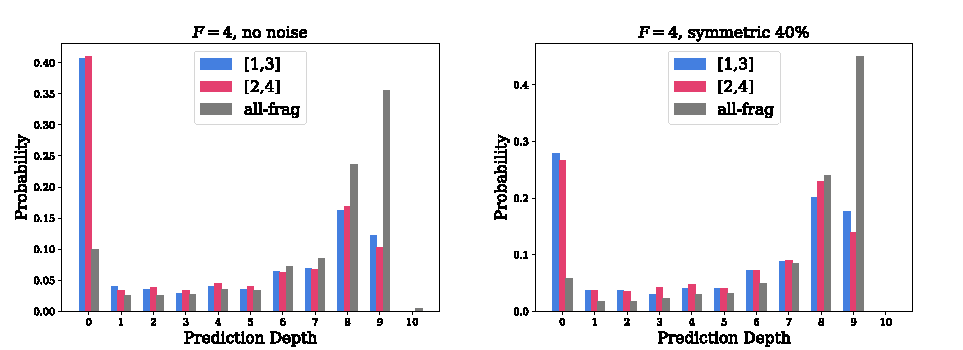
\includegraphics[width=0.8\textwidth]{imgs/pred_depth_plot_f4.pdf}}
\caption{
    \textbf{Probability of prediction depth} for examples in contrastive pairing and all-frag ($F=4$).}
\vskip -0.15in
\label{fig:pred_depth_plot_f4}
\end{center}
\end{figure*}

\begin{figure*}[th]
\begin{center}
\centerline{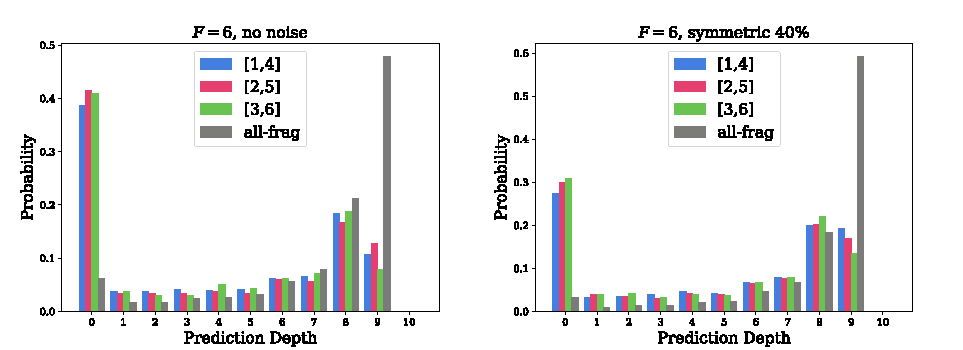
\includegraphics[width=0.8\textwidth]{imgs/pred_depth_plot_f6.pdf}}
\caption{
    \textbf{Probability of prediction depth} for examples in contrastive pairing and all-frag ($F=6$).}
\vskip -0.15in
\label{fig:pred_depth_plot_f6}
\end{center}
\end{figure*}

\section{Extended Related Work}\label{subsec:related_work}
% The unique aspect of the regression problem is that it has a continuous label space
% making it highly likely that the localities within the feature space and label space are correlated~\citep{yang21ldsfds, gong22rank, zha22supcr}.

% Recently, by exploring these characteristics, many studies have been conducted.
% They include the label imbalance problem~\citep{yang21ldsfds, gong22rank}, age estimation problem~\citep{li19bridge},
% contrastive learning~\citep{zha22supcr}, mixup regularization~\citep{yao22cmixup}.
% \citet{yang21ldsfds} proposes a label and feature distribution smoothing based on their similarity.
% \citep{gong22rank} suggests a regularization term to induce the rankings of feature-space and label-space neighbors to be in sync.
% \citet{zha22supcr} performs supervised contrastive learning using a pairing technique based on the label distances in the mini-batch.
% To use MixUp~\citep{zhang18mixup} on the regression task, \citet{yao22cmixup} proposes to interpolate the proximal samples in the label space 
% with a higher probability.

% Ordinal regression, or ranking learning, is a domain that aims to predict ordinal labels given input data.
% Regression tasks can be handled by the ordinal regression methods since the scalar label space inherently contains the numerical order.
% Previous works of the ordinal regression include solving regression problems at facial age estimation~\citep{niu2016ordinal, shin2022moving},
% monocular depth estimation~\citep{fu2018deep}, and credit rating~\citep{hirk2019multivariate}.
% Some methods share common features with our approach in that they discretize the continuous labels, converting the regression tasks into the classification tasks~\citep{niu2016ordinal, fu2018deep, shah2022label}.
% Using the framework of ordinal regression, \citet{garg2020robust} proposes a loss correction method by estimating the noise transition matrix.

% Among the methods mentioned in the previous paragraphs, only \citet{yao22cmixup, garg2020robust} can address the noisy label regression problem without additional techniques.
% In addition, \citet{wang22spr} enhanced the scalability of their approach by grouping the dissimilar classes in the feature space.
% We consider label/feature continuity and its correlation to fragment and group data.
% This way, each component can learn distinguishable features and attain a better sample selection ability. 

\subsection{Continuously Ordered Correlation of Labels and Features}\label{subsec:continuity_related_works}
One distinctive characteristic of regression problems is their continuous label space, implying a high likelihood of correlation between regions within the feature and label spaces~\citep{yang21ldsfds, gong22rank, zha22supcr}.

Recent research has extensively explored these characteristics, encompassing issues such as label imbalance~\citep{yang21ldsfds, gong22rank}, age estimation~\citep{li19bridge}, contrastive learning~\citep{zha22supcr}, and mixup regularization~\citep{yao22cmixup}. 

\citet{yang21ldsfds} propose label and feature distribution smoothing based on their similarity, while \citet{gong22rank} introduce a regularization term aimed at aligning the rankings of feature-space and label-space neighbors. 
\citet{zha22supcr} employ supervised contrastive learning with a pairing technique based on label distances in mini-batches. 
To adapt MixUp~\citep{zhang18mixup} for regression tasks, \citet{yao22cmixup} recommend interpolating proximal samples within the label space with a higher probability.

Ordinal regression, also known as ranking learning, pertains to predicting ordinal labels based on input data. 
It is noteworthy that ordinal regression methods are adaptable for regression tasks due to the inherent numerical ordering within scalar label spaces. 
Past studies in ordinal regression have successfully addressed various regression challenges, including facial age estimation~\citep{niu16afad, shin2022moving}, monocular depth estimation~\citep{fu2018deep}, and credit rating~\citep{hirk2019multivariate}. 
Some of these methods share common characteristics with our approach, as they discretize continuous labels, effectively converting regression tasks into classification problems~\citep{niu16afad, fu2018deep, shah2022label}. 
Within the framework of ordinal regression, \citet{garg2020robust} propose a loss correction method by estimating the noise transition matrix.

It is important to note that among the previously mentioned methods, only \citet{yao22cmixup} and \citet{garg2020robust} can effectively address noisy label regression problems without the need for additional techniques. 
Additionally, \citet{wang22spr} enhance the scalability of their approach by grouping dissimilar classes within the feature space. 
Our work considers the continuity of labels and features and their correlation in fragmenting and grouping data. 
This approach allows each component to learn distinguishable features and improve sample selection capabilities.


\subsection{Noisy Label in Object Detection}\label{subsec:object_detection_related_works}
Due to the abundance of research on object detection tasks, with bounding box localization being a prominent example of regression tasks,
we have explored the issue of noisy regression within the context of object detection.
In particular, obtaining accurate annotations for object detection is a resource-intensive task, often constrained by limited time, a small number of annotators, or reliance on machine-generated annotations.
These constraints frequently result in label noise, represented as incorrect class assignments or inaccurate bounding box locations.

Various strategies have been developed to address the issue of noisy labels in object detection.
To correct inaccurate bounding box locations, \citet{li2020towards} leverage the discrepancy between two classification heads by emphasizing the objectness of the region.
\citet{liu2022robust} generates object bags using the classifier as guidance, \citet{mao2021noisy} employs center-matching correction, and \citet{schubert2023identifying} drop instances with high region proposal loss on an instance-wise basis.
In scenarios where image-level annotations are available, \citet{gao2018notercnn} employs ensemble learning with two classification heads and a distillation head,
while \citet{shen2020noise} decomposes the problem into foreground and background noise, employing residual learning and bagging-mixup learning.

We also explored the possibility of applying object detection techniques to noisy labeled regression.
However, our analysis revealed that these methods are not well-suited for the broader regression task.
Specifically, \citet{liu2022robust, schubert2023identifying, mao2021noisy} utilize region proposal networks to generate bounding box proposals.
They leverage these proposals to selectively choose clean labels or re-weight the training samples.
However, because this approach necessitates an auxiliary model in the proposal generation process, it cannot be directly applied in the context of regression tasks.

Additionally, \citet{li2020towards, liu2022robust, schubert2023identifying, gao2018notercnn} employ the object detector's classifier to update or assess the quality of bounding boxes.
By evaluating the confidence or consistency of the bounding box through the classification output, this approach helps mitigate the impact of noisy labels.
However, implementing a similar approach in the context of regression tasks would require the inclusion of an auxiliary co-trained task.

\subsection{Transition Matrix based Methods}\label{subsec:transition_matrix_related_works}
Methods based on transition matrices constitute one of the primary approaches for addressing the issue of noisy labels.

Driven by the observation that the clean class posterior, denoted as $p(y^\text{gt}|x)$,
can be inferred from the transition probability and the noisy class posterior, $p(y|x)=T(y|y^\text{gt})p(y^\text{gt}|x)$,
the modification of the loss function enables the construction of a risk-consistent estimator using the estimated transition matrix~\citep{yao2020dual}.

There are many approaches aiming to enhance the estimation of the transition matrix.
These include factorizing it into the product of two matrices by introducing an intermediate class~\citep{yao2020dual}, training the Bayes label transition network~\citep{yang2021estimating},
learning the transition matrix within a meta-learning framework~\citep{wang2020training}, down-weighting less informative features based on $f$-mutual information~\citep{zhu2022beyond},
and adopting a two-head architecture. The latter involves a noisy classifier for simultaneous transition matrix estimation and a clean classifier for statistically consistent training~\citep{kye2021learning}.

Moreover, \citet{xia2020part} explores the utilization of part-dependent transition matrices, combining them to approximate the instance-dependent transition matrix.

In an extended context, \citet{li2022estimating} broadens the problem to include noisy multi-label learning and suggests considering label correlations.

\subsection{Combination with Contrastive Learning}\label{subsec:contrastive_learning_related_worls}
Incorporating unsupervised learning methods proves effective in alleviating label noise, prompting the integration of noisy label mitigation techniques with unsupervised learning, particularly contrastive learning.

\citet{zhang2021codim} show that the combination of contrastive loss and semi-supervised loss yields successful mitigation of the noisy label problem.

Beyond the application of contrastive learning, other approaches involve selecting confidence pairs and confidence samples~\citep{li2022selective},
leveraging clean probability estimation derived from the relationship between representation clusters and labels~\citep{huang2023twin},
employing class prototypes for weakly-supervised loss~\citep{li2021learning}, and implementing soft-labeling based on the relation between representations and labels~\citep{ortego2020multi}.

Additionally, an approach introduces a contrastive regularization function aimed at preventing adverse effects stemming from noisy labels~\citep{yi2022onleraning}.
% In our experiments, it performs well even if it is not specialized in noisy label learning,
% but some small-loss techniques perform better when we can use enough data.
% We also experiment the learning result by adding \cite{yao22cmixup} to the noisy label method mentioned above.

\begin{table}[t]
    \caption{\textbf{Dataset Statistics} on the six newly curated balanced datasets for regression: AFAD-B~\citep{niu16afad}, IMDB-Clean-B~\citep{lin2021imdbclean}, IMDB-WIKI-B~\citep{rothe18imdb}, UTKFace-B~\citep{zhifei2017utkface}, SHIFT15M-B~\citep{kimura21shift15m}, MSD-B~\citep{bertin11msd}.}
    \label{tab:dataset_statistics}
    \centering
    \begin{footnotesize}
    \setlength{\tabcolsep}{5pt}
    \begin{tabular}{lccccc}
        \toprule
        Dataset  & range & train & valid & test & total \\
        \midrule
        AFAD-B & [15, 40] & 27647 & 1627 & 3252 & 32526 \\
        \specialrule{0.1pt}{1pt}{1pt}
        IMDB-Clean-B & [15, 66] & 44200 & 2600 & 5200 & 52000 \\
        % \specialrule{0.4pt}{1pt}{1pt}
        % UTKFace-B~\cite{zhifei2017utkface} & [1, 70] & 9,880 & 610 & 1150 & 11,640 \\
        \specialrule{0.1pt}{1pt}{1pt}
        IMDB-WIKI-B & [15, 65] & 42500 & 2500 & 5000 & 50000 \\
        \specialrule{0.1pt}{1pt}{1pt}
        UTKFace-B & [1, 70] & 10467 & 386 & 787 & 11640 \\
        \specialrule{0.4pt}{1pt}{1pt}
        SHIFT15M-B  & [0, 40000] & 273417 & 16080 & 32180 & 321677 \\
        \specialrule{0.4pt}{1pt}{1pt}
        MSD-B & [1956, 2010] & 25218 & 1512 & 2970 & 29700 \\
        % \specialrule{0.4pt}{1pt}{1pt}
        % PovertyMap-B~\cite{yeh20povertymap}  & [-1.1, 1.4] & 9118 & 536 & 1074 & 10,728 \\
        %\specialrule{0.4pt}{1pt}{1pt}
        \bottomrule
    \end{tabular}
    \end{footnotesize}
\end{table}

\section{Experiment Details}\label{sec:exp_details}

\subsection{Dataset Curation Details}\label{subsec:dataset_curation}
Table~\ref{tab:dataset_statistics} provides a comprehensive overview of the statistics for the six benchmark datasets meticulously curated for the task of noisy label regression. 
Detailed descriptions of the dataset tailoring process are presented below for clarity.

\textbf{Age prediction datasets (IMDB-Clean-B, AFAD-B, IMDB-WIKI-B, UTKFace-B)}: These datasets are harmonized by achieving a balance across distinct age values. 
This equilibrium is established using a bin sample count threshold (clip value) of 1000 for IMDB-Clean-B and IMDB-WIKI-B, 1251 for AFAD-B, and 200 for UTKFace-B. 
Image inputs are resized to dimensions of $(128\times128)$. 
For the regression task, we consistently employ a ResNet-50 backbone across all models.

\textbf{SHIFT15M-B}: Achieving data balance in this dataset involves a two-step process. 
First, the label space is binned based on a price threshold of \textyen2000. 
Subsequently, data points exceeding the maximum price of \textyen40000 are clipped to remove outliers. 
The binning threshold is set at 16084 sample counts to further ensure balanced representation. 
To standardize the label currency, it is pegged to the U.S. dollar, referencing exchange rates from 2010 to 2020, which coincides with the period when the original clothing item data is collected. 
Notably, this dataset is provided as the penultimate feature of the ImageNet pre-trained VGG-16 model. 
Consequently, we opt for a three-layer MLP architecture with a hidden layer size of [2048, 1024, 512], aligning with recommendations from \citet{papadopoulos22fashion} and \citet{kimura21shift15m}.

\textbf{MSD-B}: Achieving balance in the Million Song Dataset involves setting a threshold of 550 samples per year. 
For all regression models in this context, we adopt a regression backbone rooted in the tabular ResNet structure proposed by \citet{gorishniy21nips}, featuring a hidden dimension of 467.

\textbf{Licenses of existing datasets. }
IMDB-Clean dataset \citep{lin2021imdbclean} is under MIT license.\footnote{\url{https://github.com/yiminglin-ai/imdb-clean}}
SHIFT15M dataset \citep{kimura21shift15m} is under CC BY-NC 4.0 and MIT license.\footnote{\url{https://github.com/st-tech/zozo-shift15m}}
MSD \citep{bertin11msd} song year prediction dataset is under CC BY 4.0 license.\footnote{\url{https://archive.ics.uci.edu/dataset/203/yearpredictionmsd}}
UTKFace dataset \citep{zhifei2017utkface} is available for non-commercial research purposes only.\footnote{\url{https://susanqq.github.io/UTKFace/}}
IMDB-WIKI dataset \citep{rothe2015imdb-wiki,rothe18imdb} is available for academic research purpose only.\footnote{\url{https://data.vision.ee.ethz.ch/cvl/rrothe/imdb-wiki/}}
Unfortunately, the license of AFAD \citep{niu16afad} dataset could not be found.\footnote{\url{https://github.com/John-niu-07/tarball}}

\subsection{Baselines Details}\label{subsec:baselines}
While numerous branches of noisy labeled learning have been explored for classification tasks, our focus in this study centers on the challenging domain of noisy label regression. 
To comprehensively investigate this task, we have conducted an extensive review of the various branches and have selected a set of fourteen baselines that are adaptable to regression. 
It is worth noting that C-Mixup~\citep{yao22cmixup} was originally proposed as a regression baseline.
In the following section, we provide an overview of these selected baselines, offering a broad coverage of diverse approaches to address the noisy label regression problem. 
Additionally, we present detailed descriptions of the experimental settings for each baseline.

\begin{enumerate}
\item D2L~\citep{ma18d2l} for intrinsic dimension exploration. Following the paper, we set $k=20$ and $m=10$ for Local Intrinsic Dimensionality (LID) estimation
and set the LID estimation window as five following the official implementation.
\item CDR~\citep{xia21cdr} for model weight parameter selection, and RDI~\citep{hu20rdiaux} for regularizing the paramter distance from the initialization.
At RDI, we use search space $\lambda \in [0.25, 0.5, 1, 2, 4, 8]$.
\item C-Mixup~\citep{yao22cmixup} for regularization via continuous mixup.
C-Mixup-batch is used in all experiments because of the excessive memory requirement for pairwise distance matrix $P$.
We set the beta distribution variable $\alpha$ as 1.5.
The bandwidth variable $\sigma$ is searched over [0.01, 0.1, 1], following~\citet{yao22cmixup}.
\item SELFIE~\citep{song19b} and AUX~\citep{hu20rdiaux} for refurbishing.
To apply SELFIE to the continuous label, we redefine the concept of uncertainty $F(x;q)$ and
refurbished labels $y^{refurb}$ with the mean and standard deviation.
\begin{align}\label{eq:selfie_uncertainty}
    F(x;q) = \frac{\sigma(H_x(q))}{(\max{(Y)}-\min{(Y)})} < \epsilon
\end{align}
\begin{align}\label{eq:selfie_refurbished_label}
    y^{refurb} = \mu(H_x(q))
\end{align}
where $H_x(q)$ is the prediction history of $x$ from before $q$ epochs, $\epsilon$ is the uncertainty threshold.

For SELFIE, we train 1/4 of the total training epochs for the warm-up phase, following~\citet{song19b}.
The variable $q$ is searched over half of the warm-up epochs and around.
The variable $\epsilon$ is searched over [0.05, 0.10, 0.15, 0.20], following~\citet{song19b}.
% For Co-Selfie, we search over the same parameters as Co-ConFrag.


For AUX~\citep{hu20rdiaux}, we regularize the auxiliary variable by weight decay 0.0005, reducing the weight by 0.1 at 1/2 and 3/4 of the total training epochs.
The learning rate of the auxiliary variable is set to 0.1 and 0.01.
The variable $\lambda$ is searched over [0.25, 0.5, 1, 2, 4, 8].
\item SPR~\citep{wang22spr} performs penalized regression for selection. It requires some adaptation to regression by ignoring the $\ell_q$
penalty as there is no longer a linearity gap between the scalar output and the final fully connected layer that requires reducing.
Also, we use our fragmentation splits $\{4, 8\}$ to bin the regression data for SPR's parallel optimization.
\item Sigua~\citep{han20sigua} and CNLCU-S/H~\citep{xia22} for small loss selection.
For Sigua, we use $\delta(t)\in[0.3, 0.4]$ and $\gamma=0.01$ and set $T_k$ as 5\% of the total training epochs.
For CNLCU-S/H, we search $\sigma$ and $\tau_{\min}$ in [0.01, 0.1, 1, 10] and set $T_k$ as 5\%.

\item BMM~\citep{arazo19} for selection based on beta mixture model fitting on the loss distribution. 
BMM does hard sampling and trains using the selected samples.
DY-S is a dynamic soft loss. We implemented two versions; the first uses a convex combination as in \citet{reed15} $((1-w)\tilde{y}^c - w\hat{y})^2$. Second, instead of bootstrapping, we dynamically weight the loss using the BMM probability to create a cost-sensitive loss, $(1-w)\ell$.
The $w$ is the mixture clean probability, $\hat{y}$ is the model prediction, $\tilde{y}^c$ is the assigned noisy label, and $\ell$ is the loss.

\item SuperLoss~\citep{castells20} regularization parameter $\lambda$ is searched over [0.01, 0.1, 1, 10] while $\tau$ uses an exponential running average with a fixed smoothing parameter $\alpha = 0.9$.

\item \text{[Incompatible]} CRUST~\citep{mirzasoleiman20crust} for clean coreset selection.
It aims to select a coreset based on \textit{class-wisely gradient clustering}.
% For regression, we viewed all data as a single class and proceeded with coreset selection.
For regression, we initially viewed \textit{all data as a single class} and proceeded with coreset selection, but the results were unsatisfactory.
Therefore, we report results based only on the discretized version, demonstrating comparable performances.
We select 1/2 of the total dataset as a coreset.
The distance threshold in calculating clusters is searched over [1, 2, 4].

\item \text{[Incompatible]} OrdRegr~\citep{garg2020robust} for loss correction.
Since no official implementation is provided, we implemented it with cross-entropy loss for ordinal regression.
Importantly, we failed to find accurate noise rate estimation using their suggested methods.
Even when considering the transition matrix with the actual noise rate, the loss correction algorithm proved ineffective in our benchmark tests.

\end{enumerate}

\subsection{ConFrag Training Details}\label{subsec:training_details}
% FragSel-R's regression feature extractor employs the standard Mean Squared Error (MSE) loss.
% For FragSel, the discriminator feature extractor utilizes the Symmetric Cross Entropy (SCE) loss~\citep{wang19sce}, configured with specific parameters: $\alpha=10.0$ and $\beta$ in the range of $[0.1, 1.0]$. 
% Additionally, mixup~\citep{zhang18mixup} is incorporated into the training process with a parameter value of $\alpha=1.0$ to enhance model robustness.
% Both FragSel and FragSel-R employ the Cosine Annealing Learning rate~\citep{loshchilov17iclr} with a minimum learning rate of $\eta_{min}=0$.

% ConFrag utilizes two distinct classification approaches for classification when assessing self-agreement and neighborhood agreement in Eq.~\ref{eq:self_agreement}--~\ref{eq:na_final}, each utilizing different aspects of the expert feature extractors.
% First is using \textit{predictive} aspect, in which we use the binary classifier of the feature extractor learned during the training in \S~\ref{subsec:training_feature_extractors}, which is a linear classifier on the learned feature space.
% Second is using \textit{representational} aspect, where we use non-linear $K$-nearest neighbor classifier on the feature space learned by the expert.
% Using these two distinct classification approaches, we obtain respective sample probability (Eq.~\ref{eq:mcf}): predictive $p^p(\cdot)$ and representational $p^r(\cdot)$.
% Subsequently, we sample $\mathcal{S}^p$ and $\mathcal{S}^r$ from $p^p(\cdot)$ and $p^r(\cdot)$, respectively.
% Finally, the union of $\mathcal{S}^p$ and $\mathcal{S}^r$ is used as the clean set $\mathcal{S}$.
% By utilizing different aspect of the learned expert and two distinct classification approaches (linear and non-linear), we further improve the performance of ConFrag, as shown in Appendix~\ref{subsec:ablation}.

ConFrag employs the Cosine Annealing Learning rate~\citep{loshchilov17iclr} with a minimum learning rate of $\eta_{min}=0$.
The optimization is carried out using the Adam optimizer~\citep{kingma15adam}.
For the $K$-nearest neighbors-based prediction, we experiment with various values of $K$, specifically choosing from the set $[3, 5, 7]$. 
The number of fragments, denoted as $F$, remains constant at four throughout all the experiments. 
To determine the buffer range for jittering, we conduct a search over values within the range $[0, 0.05, 0.1]$.



Some dataset-specific hyperparameters exist:
\begin{itemize}
    \item Age prediction task datasets, IMDB-Clean-B~\citep{lin2021imdbclean}, AFAD-B~\citep{niu16afad}, IMDB-WIKI-B~\citep{rothe18imdb}, and UTKFace-B~\citep{zhifei2017utkface}, train for 120 epochs
    % with learning rate of 0.01 and weight decay of 0.0005 for FragSel-R, and learning rate of 0.001 and weight decay of 0.0005 for FragSel. 
    with a learning rate of 0.001. 
    Each feature extractor employs the ResNet-18 architecture, which contains only 48\% of the parameters found in ResNet-50, the architecture utilized for the regressor.
    \item Clothing price estimation task dataset SHIFT15M-B~\citep{kimura21shift15m} trains for 40 epochs
    % with learning rate of 0.001 and weight decay of 0.1 for FragSel-R, and learning rate of 0.0001 and weight decay of 0.05 for FragSel.
    with a learning rate of 0.0001.
    MLP with hidden dimensions [1024, 512, 256] is deployed for feature extractors, and the parameter size is 44\% of the regressor.
    \item Music year production task dataset MSD-B~\citep{bertin11msd} trains for 20 epochs
    % with learning rate of 0.01 and weight decay of 0.1 for FragSel-R and learning rate of 0.0001 and weight decay of 0.05 for FragSel. 
    with a learning rate of 0.0001. 
    Similar to the regression backbone, the feature extractor model is the tabular ResNet structure\citep{gorishniy21nips}, and the hidden dimension is reduced to 256.
\end{itemize}

\begin{figure}[t]
\begin{center}
\centerline{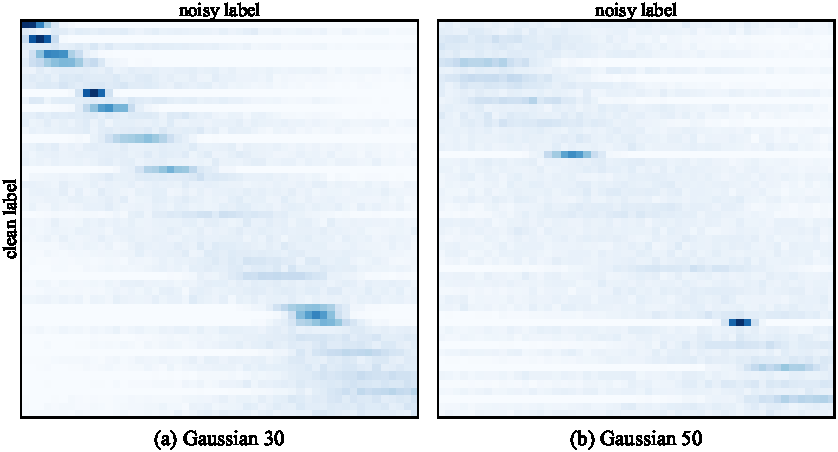
\includegraphics[width=0.8\columnwidth]{imgs/gaussian_noise_depict.pdf}}
\caption{\textbf{Random Gaussian Noise.} (a) Gaussian noise injected from the uniformly sampled random standard deviation between $[1,30]$. 
(b) Gaussian noise injected from uniformly sampled random standard deviation between $[1,50]$.}
\label{fig:gaussian_depict}
\end{center}
\end{figure}

\subsection{Random Gaussian Noise}\label{subsec:random_gaussian}
Fig.~\ref{fig:gaussian_depict} illustrates the application of random Gaussian noise within the label space of IMDB-Clean-B~\citep{lin2021imdbclean}. 
The procedure for injecting noise is akin to the approach employed by \citet{yao22cmixup}, where Gaussian noise is applied to every unique label within the training samples. 
Specifically, \citet{yao22cmixup} sets the standard deviation of the Gaussian noise as a fixed 30\% of the range of the label space corresponding to the dataset. 
In contrast, our noise injection method introduces an element of stochasticity, allowing for variable levels of deviation for each unique label.

To achieve this variability, we employ uniform sampling from the minimum and maximum values specific to each label's domain. 
For instance, in the context of an age prediction task, we assume minimum and maximum values of 0 and 100, respectively. 
However, in cases where the label domain lacks clarity (\eg for a variable like `price'), we utilize the minimum and maximum label values provided by the dataset itself.

It is important to highlight that baselines with known noise rates, such as CNLCU-S/H, Sigua, and Selfie, are incapable of dealing with Gaussian noise.
Given that these baselines employ a heuristic approach to control selection rates through $(1 - \text{noise rate})$,
they prove ineffective when exposed to Gaussian noise, as it introduces noise to all samples, thereby resulting in a nearly 100\% noise rate.
Hence, we create a \emph{soft noise rate} to be used by them for selection.
This is done by calculating an updated noise rate, assuming that the Gaussian noise injected samples that fall within an acceptable variance of the original ground-truth label are clean
(the acceptable variance is set to equal the label length/size of a single fragment).

\subsection{Computation Resource}\label{subsec:computation_resource}

For implementation, we use Python 3.9 and PyTorch 1.13.1.
All experiments are conducted using NVIDIA Quadro 6000 24GB RAM GPUs.
The required computation time for experiments differs depending on the dataset.
Below, we report the computation time for each dataset.

\textbf{AFAD-B. }
On the AFAD-B dataset, the average computation time of ConFrag and Co-ConFrag are approximately 2.5 GPU hours and 5 GPU hours, respectively.
The computation time of baselines ranges from 1.25 GPU hours to 4 GPU hours.
About 650 GPU hours were required to produce the AFAD-B part of Tab.~\ref{tab:main_mrae}.


\textbf{IMDB-Clean-B. }
On the IMDB-Clean-B dataset, the average computation time of ConFrag and Co-ConFrag are approximately 3.5 GPU hours and 5.5 GPU hours, respectively.
The computation time of baselines ranges from 2 GPU hours to 5 GPU hours.
About 970 GPU hours were required to produce the IMDB-Clean-B part of Tab.~\ref{tab:main_mrae}.

\textbf{SHIFT15M-B. }
On the SHIFT15M-B dataset, the average computation time of ConFrag and Co-ConFrag are approximately 1 GPU hour and 1.2 GPU hours, respectively.
The computation time of baselines ranges from 6 GPU minutes to 1 GPU hour.
About 100 GPU hours were required to produce the SHIFT15M-B part of Tab.~\ref{tab:main_mrae}.


\textbf{MSD-B. }
On the MSD-B dataset, the average computation time of ConFrag and Co-ConFrag are approximately 4 GPU minutes and 5 GPU minutes, respectively.
The computation time of baselines ranges from 1 GPU minute to 4 GPU minutes.
About 9 GPU hours were required to produce the MSD-B part of Tab.~\ref{tab:main_mrae}.

Additionally, further computation was required for analysis and experiments in \S~\ref{sec:discussion} and Appendix~\ref{sec:results_analysis}.


\section{Extended Results \& Analysis}\label{sec:results_analysis}
% We perform additional experiments and analysis in terms of fragment numbers, ablation, and combination with other baselines for FragSel, compare the 
% discretized baselines performances, ERR analysis on the Gaussian random noise, as well as perform additional fragment number analysis on the clothing price domain, and lastly, analyze how our algorithm handles the anomalies post fragmentation.
We conduct supplementary experiments and analyses of UTKFace dataset, parameter sizes, fragment numbers ($F$), other hyperparameters ($K$, $J$), fragment pairing, and the impact of closed-set and open-set noise.
Furthermore, we present ablation analyses, comparisons with discretized baselines, baseline performance evaluations considering Selection rate and ERR, variance assessments,
and the obtained MAE results.


\subsection{UTKFace Results}\label{subsec:utkface} % The analysis shows a stark tradeoff between selection versus refurbishing and that FragSel’s cost of refurbishing 
Table~\ref{tab:utkface} presents a comparison of MRAE values between various baseline methods and our proposed approach on the balanced UTKFace dataset~\citep{zhifei2017utkface}, UTKFace-B. 
We experiment under four different symmetric noise conditions of symmteric 20\%, 40\%, 60\% and 80\% noise rates.
Both ConFrag and Co-ConFrag demonstrate superior performance across all experiments when compared to the fourteen baseline methods.


\begin{table*}[t]
    \centering
    \caption{Comparison of MRAE (\%) on UTKFace-B datasets with symmetric noise.}
    \begin{small}
    \setlength{\tabcolsep}{4.2pt}
    \begin{tabular}{lcccc}
    \toprule
    &\multicolumn{4}{c}{\textbf{UTKFace-B}} \\
    \cmidrule(lr){2-5}
    &\multicolumn{4}{c}{symmetric} \\
    \cmidrule(lr){2-5}
    \textbf{} & 20 & 40 & 60 & 80 \\
    \midrule
    Vanilla &  37.59 & 53.96 & 82.88 & 115.49 \\
    AUX &  25.53 & 48.01 & 84.78 & 118.31 \\
    BMM &  49.21 & 76.25 & 88.87 & 139.01 \\
    CDR & 32.87 & 50.56 & 83.41 & 121.36 \\
    C-Mixup &  17.76 & 34.00 & 74.29 & 117.68 \\
    CNLCU-H &  \textcolor{blue}{5.75} & 20.75 & 43.44 & 121.55 \\
    CNLCU-S &  20.29 & 36.69 & 43.44 & 121.55 \\
    D2L & 38.28 & 51.22 & 99.19 & 122.50 \\
    DY-S & 22.73 & 31.07 & 58.05 & 113.21 \\
    RDI & 43.49 & 49.44 & 75.67 & 122.40 \\
    Selfie & 30.47 & 44.62 & 99.67 & 130.97 \\
    Sigua &  10.86 & 19.58 & 52.37 & 128.06 \\
    SPR &  28.05 & 48.07 & 85.18 & 120.58 \\
    Superloss & 9.12 & 22.10 & 55.78 & 115.78 \\
    \specialrule{0.7pt}{1pt}{1pt}
    ConFrag &  6.28 & \textcolor{blue}{14.30} & \textcolor{blue}{34.09} & \textcolor{blue}{83.03} \\
    Co-ConFrag & \textcolor{red}{-2.22} & \textcolor{red}{8.88} & \textcolor{red}{25.46} & \textcolor{red}{74.78} \\
    \bottomrule
    \end{tabular}
    \end{small}
    \label{tab:utkface}
\end{table*}


% \begin{wrapfigure}{r}{0.5\columnwidth}
% \begin{center}
% \vskip -0.1in
% 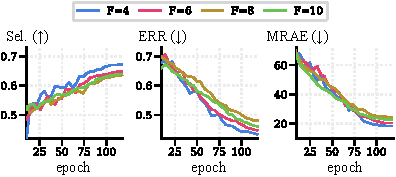
\includegraphics[width=0.5\columnwidth]{imgs/split_analysis_small.pdf}
% \vskip -0.1in
% \caption{\textbf{Fragment number analysis} compares the Selection rate, ERR and MRAE on IMDB-Clean-B with symmetric 40\% noise.}
% \label{fig:split_number}
% \end{center}
% \vskip -0.1in
% \end{wrapfigure}

\begin{figure*}[th]
\begin{center}
\centerline{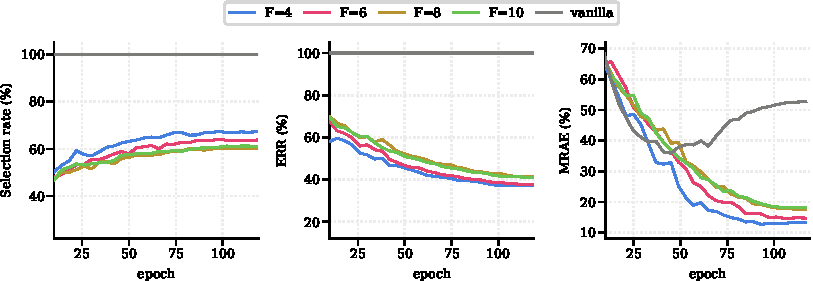
\includegraphics[width=\textwidth]{imgs/split_analysis_wide.pdf}}
\caption{\textbf{Fragment number analysis} compares the Selection rate, ERR and MRAE on IMDB-Clean-B with symmetric 40\% noise.}\label{fig:split_number}

\end{center}
\end{figure*}

\begin{figure*}[th]
\begin{center}
\centerline{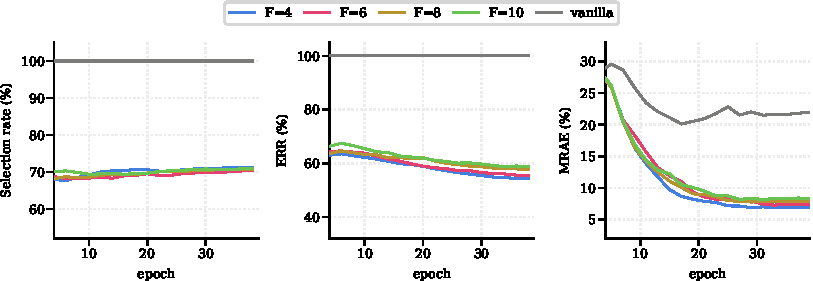
\includegraphics[width=\textwidth]{imgs/split_analysis_wide_shift.pdf}}
\caption{\textbf{Fragment number analysis} compares the Selection rate, ERR and MRAE on SHIFT15M-B with symmetric 40\% noise.}\label{fig:split_number_shift}

\end{center}
\end{figure*}

% \begin{figure*}[t]
% \begin{center}
% \centerline{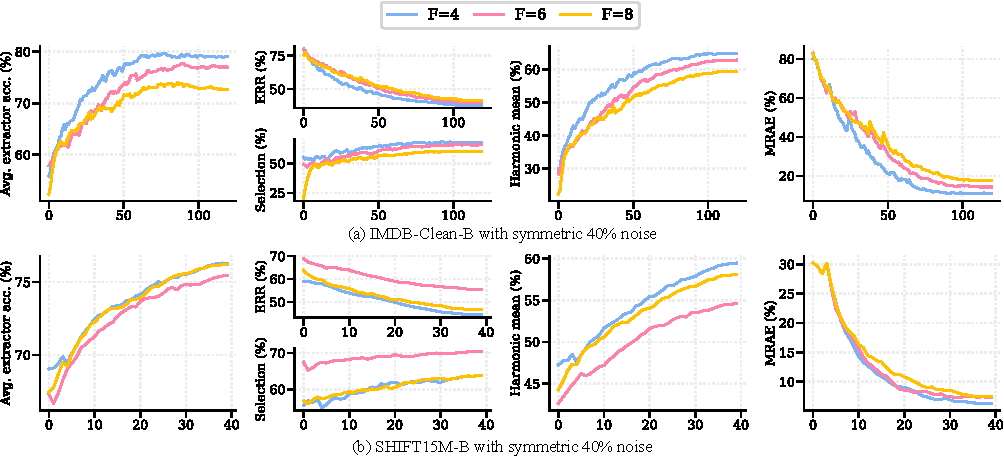
\includegraphics[width=\textwidth]{imgs/fragment_num_analysis.pdf}}
% % \vskip -0.15in
% \caption{\textbf{Fragment number anaylsis.}
% Performance of the experiments when $F=[4,6,8]$. 
% % We show the harmonic mean of $(1-ERR)$ and Selection. 
% % Based on the harmonic mean of the extractor's filtering performance, we can approximate downstream task performance. 
% % This allows us to efficiently select the hyperparameter F without the need for downstream task training.
% }
% \label{fig:fragnum_analysis}
% \end{center}
% \vskip -0.25in
% \end{figure*}

\subsection{Fragment Number Analysis}\label{subsec:fragment_numbers} % The analysis shows a stark tradeoff between selection versus refurbishing and that FragSel’s cost of refurbishing 
% is much greater. This hints that alternatively utilizing semi-supervised techniques~\cite{spr, dividemix, etc} 
% could bring much further improvements.
% Fig.~\ref{fig:split_number} analyzes the variation of clean selection, refurbishment, and the discriminative model's test 
% accuracy according to fragment numbers based on the best MRAE performance. Fragment four performs the best in this experiment setting (IMDB-Clean-B with 40\% symmetric noise).
% The possible reasons why the performance drops after a certain number of fragments are as follows. The amount of training data per discriminative model decreases 
% with an increase in fragment size and also, the tradeoff between clean selection and refurbishing as seen in Fig.~\ref{fig:split_number} (a), (b) shows the negative correlation of the two for selection as well as the average error.
% The analysis indicates that FragSel's cost of refurbishing is much greater. 
% This hints that alternatively, utilizing semi-supervised techniques~\citep{wang22spr,li2020dividemix} could further improve our approach.
% The Appendix includes the fragment analysis of some other datasets on different domains.
% Choosing an optimal number of fragments is a challenging task involving the tradeoff of task difficulty [1,2] and instance difficulty [3, 4, 5], as well as the data size. 
% Choosing an optimal \textit{total} number of fragments depends on dataset difficulty~\citep{ethayarajh22icml}, an area that is beginning to receive attention.
% In this work, we assume the simplest setting by fixing the total fragment number as four and still see significant performance improvements in all our experiments.

% In Fig.~\ref{fig:split_number}, \ref{fig:split_number_shift}, we conduct an analysis of various fragment numbers in the context of symmetric 40\% noise within the IMDB-Clean-B and SHIFT15M-B benchmarks.
% We compare the Selection rate, ERR, and MRAE to evaluate the performance.
% Overall, a decline in performance is seen in IMDB-Clean-B with increasing fragments, while relatively consistent performance is seen in SHIFT15M-B no matter the fragment number.
% Furthermore, the observed decline in performance when the number of fragments increases is likely due to a finer division of training data per feature extractor (discriminative model), leading to reduced generalization performance.

% The choice of an optimal \textit{total} number of fragments is contingent upon the dataset's inherent difficulty, an aspect that is garnering increasing attention in the research community~\citep{ethayarajh22icml}. 
% In this study, we adopt the simplest configuration by setting the total number of fragments to four, and yet, we consistently observe significant improvements in performance across all our experiments.

In Fig.~\ref{fig:split_number} and \ref{fig:split_number_shift}, we undertake an examination of various fragment numbers within the context of symmetric 40\% noise, using the IMDB-Clean-B and SHIFT15M-B datasets as benchmarks. 
Our evaluation criteria encompass the Selection rate, Error Residual Rate (ERR), and Mean Relative Absolute Error (MRAE).
The number of fragments is chosen from $F\in[4, 6, 8, 10]$.
To address scenarios with a smaller fragment number, we examine cases where $F=1$ or $2$.
When $F=2$, a fragment $f$ that satisfies self-agreement (Eq.~\ref{eq:self_agreement}) does not meet the criteria for neighbor-agreement ($\alpha^\text{ngb}_f$ in Eq.~\ref{eq:na_final}),
as the agreement relies on comparing the distribution of fragment $f$ and its contrasting pair $f^+$.
Consequently, the unified neighborhood agreement (Eq.~\ref{eq:na_final}) consistently yields a value of $0$.
On the other hand, defining a contrasting pair is not feasible when $F=1$.
% As a result, the computation of the distribution (Eq.~\ref{eq:score}) becomes unfeasible,
% thereby rendering the calculation of neighborhood agreement (Eq.~\ref{eq:na_final}) not possible.
Instead, we present a plot of the vanilla baseline to illustrate the case when $F=1$ without utilizing ConFrag.

The results reveal that the MRAE of the vanilla model initially decreases during the early epochs as it learns patterns from clean samples.
However, as the model starts to memorize noisy samples, the MRAE degrades.
In contrast, ConFrag consistently mitigates the impact of noisy samples across all plots ($F\in[4,6,8,10]$) when compared to the vanilla baseline.

We also observe a declining trend in performance as the number of fragments increases in the case of IMDB-Clean-B. 
In contrast, SHIFT15M-B exhibits relatively stable performance across different fragment numbers. 
% This decrease in performance with an increased number of fragments is likely attributed to a finer division of the training data among feature extractors (discriminative models), ultimately leading to reduced generalization capabilities.
This decrease in performance with an increased number of fragments is likely attributed to a finer division of the training data among feature extractors, ultimately leading to overfitting and reduced generalization capabilities.

% There is room for further improvements by considering the algorithmic updates with increasing fragment numbers.
% The results are encouraging in that there is room for further improvements by tuning the fragment number, as well as algorithmic updates with increasing fragment numbers could also be considered.
% The analysis shows that increasing the number of fragments leads to much-improved results.
% Additionally, the main possible reason for the performance drop in the IMDB-Clean-B experiments with an increasing number of fragments is likely due to the finer division of training data per feature extractor (discriminative model), ultimately leading to a decline in the generalization performance. 
% We \textit{fix the fragment number to four in all experiments}, but
% This hints that alternatively, utilizing semi-supervised techniques~\citep{wang22spr,li2020dividemix} could further improve our approach.

% \begin{figure}[h]
%     \begin{minipage}[t]{.49\textwidth}
%     \begin{center}
%     \centerline{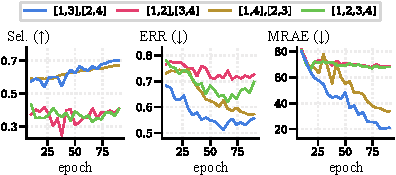
\includegraphics[width=\linewidth]{imgs/fragmentation_analysis.pdf}}
%     \caption{
%     \textbf{Contrasting Fragment combination analysis} compares contrastive pairings ([1,3], [2,4]), other pairings,
%     and all-fragments ([1,2,3,4]) on IMDB-Clean-B with 40\% symmetric noise.
%     All pairings use ResNet-18, while all-fragments use a ResNet-34 backbone.
%     % TODO: if this figure is relocated to Section 2, rename it
%     }
%     \label{fig:contrasting_fragments}
%     \end{center}
%     \end{minipage}
%     \hspace{0.02\textwidth}
%     \begin{minipage}[t]{.49\textwidth}
%     \begin{center}
%     \centerline{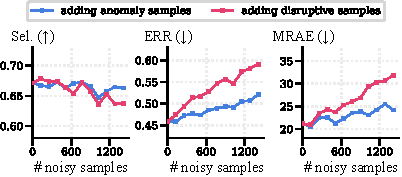
\includegraphics[width=\linewidth]{imgs/disruptive_analysis.pdf}}
%     \caption{
%     \textbf{Disruptive/anomaly noise analysis} displays the selection, ERR score and MRAE
%     when disruptive or anomaly noisy samples are injected into the clean dataset.
%     The experiments are based on IMDB-Clean-B.
%     % TODO: if this figure is relocated to Section 2, rename it
%     }
%     \label{fig:disruptive_analysis}
%     \end{center}
%     \end{minipage}
% \end{figure}
\begin{figure*}[th]
\begin{center}
\centerline{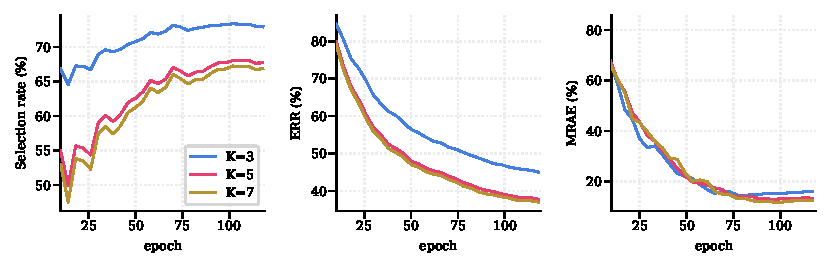
\includegraphics[width=\textwidth]{imgs/hp_analysis_imdb_k.pdf}}
\vskip -0.15in
\caption{
    \textbf{Hyperparameter K analysis} compares the Selection rate, ERR and MRAE on IMDB-Clean-B with symmetric 40\% noise.}
    \label{fig:analysis_imdb_k}
\vskip -0.15in
\end{center}
\end{figure*}

\begin{figure*}[th]
\begin{center}
\centerline{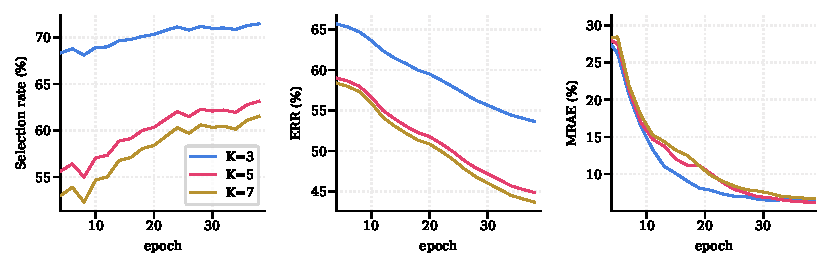
\includegraphics[width=\textwidth]{imgs/hp_analysis_shift15m_k.pdf}}
\vskip -0.15in
\caption{
    \textbf{Hyperparameter K analysis} compares the Selection rate, ERR and MRAE on SHIFT15M-B with symmetric 40\% noise.}
\vskip -0.15in
\label{fig:analysis_shift15m_k}
\end{center}
\end{figure*}

\begin{figure*}[th]
\begin{center}
\centerline{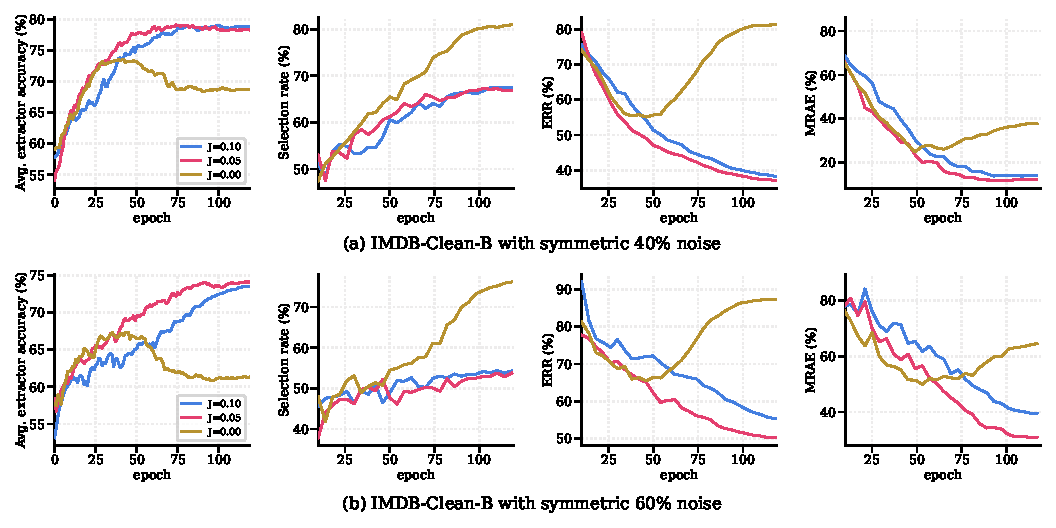
\includegraphics[width=\textwidth]{imgs/hp_analysis_imdb_j.pdf}}
\vskip -0.15in
\caption{
    \textbf{Hyperparameter J analysis} compares the average accuracy of feature extractors, the Selection rate, ERR and MRAE on IMDB-Clean-B with symmetric 40\%, 60\% noise.}
\label{fig:analysis_imdb_j}
\end{center}
\end{figure*}

\begin{figure*}[th]
\begin{center}
\centerline{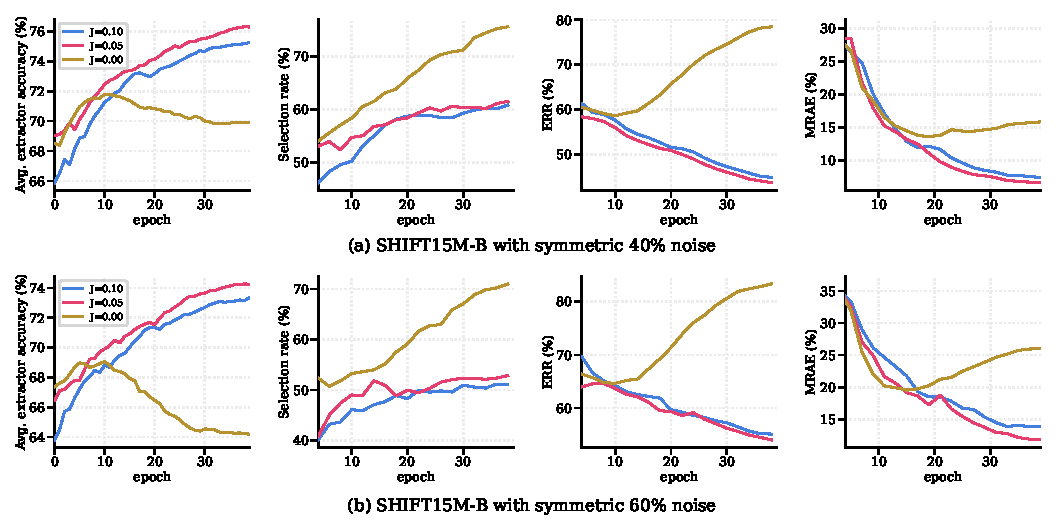
\includegraphics[width=\textwidth]{imgs/hp_analysis_shift15m_j.pdf}}
\vskip -0.2in
\caption{
    \textbf{Hyperparameter J analysis} compares the average accuracy of feature extractors, the Selection rate, ERR and MRAE on SHIFT15M-B with symmetric 40\%, 60\% noise.}
\label{fig:analysis_shift15m_j}
\end{center}
\end{figure*}

\subsection{Hyperparameter Analysis}\label{subsec:hyperparameter}
% The hyperparameter $K$ is used for determines the number of neighbors considered when assessing self/neighbor agreement from a representation perspective.
The hyperparameter $K$ is used for $K$-nearest neighbor classification when assessing self/neighbor agreement from a representational perspective.
As shown in Fig.~\ref{fig:analysis_imdb_k}, \ref{fig:analysis_shift15m_k}, with an increase in the value of $K$, the criteria for agreement become more stringent.
Consequently, as the value of $K$ increases, a greater number of confident samples are selected, resulting in a reduction in the Selection rate and ERR. 

The hyperparameter $J$ controls the buffer range for jittering, which, in turn, determines the level of regularization applied via neighborhood jittering.
Increasing the value of $J$ results in stronger regularization, effectively preventing overfitting. 
However, excessive regularization, as observed when $J = 0.10$, may result in adverse effects during training.
Specifically, in Fig.~\ref{fig:analysis_imdb_j}(a), the feature extractors exhibit similar convergence patterns when $J = 0.05$ or $J = 0.10$. 
Consequently, comparable performance is observed in Selection Rate and MRAE.
Yet, in Fig.~\ref{fig:analysis_imdb_j}(b), the ERR of $J = 0.05$ is smaller than that of $J = 0.10$, leading to improved MRAE performance for $J=0.05$. 
% As a result, the slow convergence phenomenon with larger $J$ values that can occur with the same training time leads to relatively lower MRAE performance.
Similar effects are observed in the SHIFT15M dataset, as depicted in Fig.~\ref{fig:analysis_shift15m_j} (SHIFT15M-B).


\begin{figure*}[th]
\begin{center}
\centerline{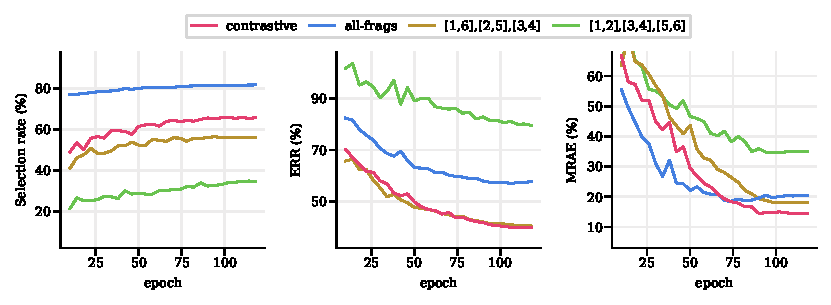
\includegraphics[width=\textwidth]{imgs/fragmentation_analysis_wide.pdf}}
\vskip -0.2in
\caption{
% \textbf{Contrasting Fragment combination analysis} compares contrastive pairings ([1,4], [2,5], [3,6]) and two versions of all-fragments ([1,2,3,4,5,6]) on IMDB-Clean-B with 40\% symmetric noise.
% Contrastive pairings use ResNet-18, while all-fragments use a ResNet-34 backbone.
% }
\textbf{Fragment pairing analysis} compares contrastive pairings ($[1,4], [2,5], [3,6]$), all-fragments ($[1,2,3,4,5,6]$),
and alternative pairing methods ($[1,2],[3,4],[5,6]$ and $[1,6],[2,5],[3,4]$) on IMDB-Clean-B with 40\% symmetric noise when $F=6$.
For feature extractor, all-fragments use a ResNet-34, while other pairing methods use ResNet-18 backbones.
}
\label{fig:contrasting_fragments}
\end{center}
\end{figure*}

\begin{figure*}[th]
\begin{center}
\centerline{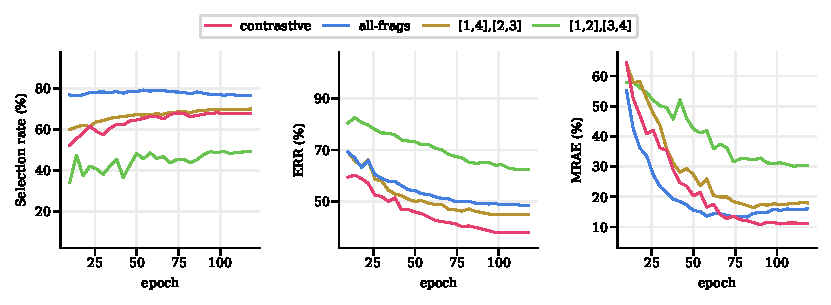
\includegraphics[width=\textwidth]{imgs/fragmentation_analysis_wide_f4_full.pdf}}
\vskip -0.2in
\caption{
% \textbf{Contrasting Fragment combination analysis} compares contrastive pairings ([1,4], [2,5], [3,6]) and two versions of all-fragments ([1,2,3,4,5,6]) on IMDB-Clean-B with 40\% symmetric noise.
% Contrastive pairings use ResNet-18, while all-fragments use a ResNet-34 backbone.
% }
\textbf{Fragment pairing analysis} compares contrastive pairings ($[1,3], [2,4]$), all-fragments ($[1,2,3,4]$),
and alternative pairing methods ($[1,2],[3,4]$ and $[1,4],[2,3]$) on IMDB-Clean-B with 40\% symmetric noise when $F=4$.
For feature extractor, all-fragments use a ResNet-34, while other pairing methods use ResNet-18 backbones.
}
\label{fig:contrasting_fragments_f4}
\end{center}
\end{figure*}

% DY: this figure is relocated from main paper to supp. need to be included in the paragraph
\begin{figure}[t]
    \begin{center}
    \centerline{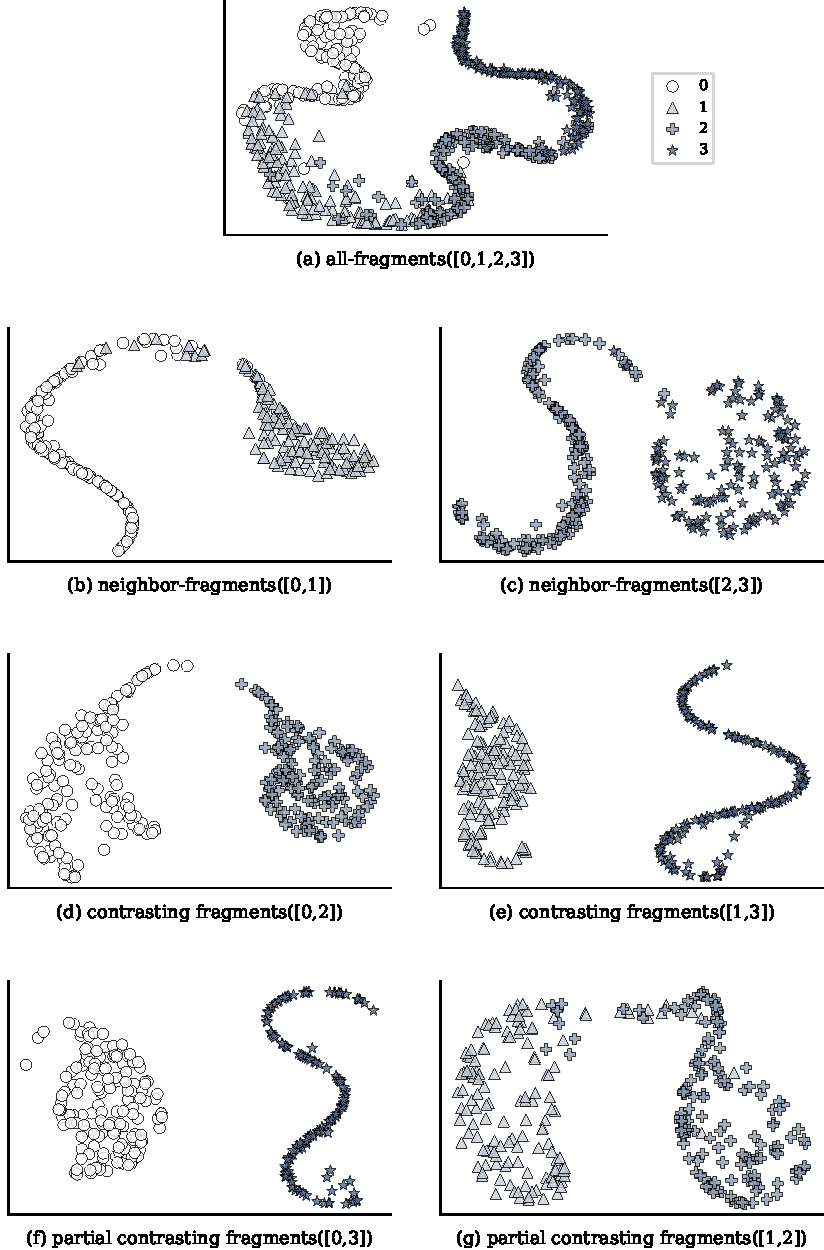
\includegraphics[width=0.7\columnwidth]{imgs/fragment_tsne.pdf}}
    \caption{\textbf{Detailed Representation Depiction}.
    A detailed comparison of the effect of fragment pairings via t-SNE visualization of the penultimate features from the feature extractors.
    % (a)-(b) train the two models with contrasting fragments (i.e., [0,2], [1,3]).
    % (c)-(d) train the two models with neighboring fragments (i.e., [0,1], [2,3]).
    % (e)-(f) train the two models with contrasting and neighboring fragments (i.e., [0,3], [1,2]).
    % (g) trains a single model with all fragments. 
    The experiments are based on IMDB-Clean-B.
    }
    \label{fig:feature_space_depict}
    \end{center}
    \vskip -0.1in
\end{figure}



\subsection{Fragment Pairing Analysis}\label{subsec:contrast_combination}
% In Fig.~\ref{fig:fragment_motivation}(b), we provide further insight into our approach by comparing contrasting fragments ($[1,4], [2,5], [3,6]$) with all-fragments ($[1,2,3,4,5,6]$). 
% Since the discriminators for all-fragments are not trained using contrastive pairs, we assume that an agreement ($\alpha_f^\text{self}==1$) in the predictive space is achieved if the likelihoods ($p(f|x;\theta)$) for both the self and the neighbor(s) are ranked within the top half.

% We consider two variations: the `or' version, which counts an agreement when either the left \textit{or} right neighbor is in the top half, and the `and' version, which requires both the left \textit{and} right neighbors to be in the top half. 
% In Fig.~\ref{fig:fragment_motivation}(b), we report the `and' version since it exhibits superior performance in terms of Mean Relative Absolute Error (MRAE).

% The evaluation metrics, including the Selection rate, Error Residual Rate (ERR), and MRAE, consistently demonstrate that contrasting fragment pairs outperform both types of all-fragments outcomes. 
% Importantly, for an optimal selection algorithm, the Selection rate should approach $100 - \text{noise rate}(\%)$, while ERR and MRAE should be minimized. 
% The results unequivocally indicate that contrasting fragments offer significant advantages as a selection algorithm.

In Fig.~\ref{fig:fragment_motivation}(c), we offer deeper insights into our approach by comparing contrastive fragment pairing ($[1,4], [2,5], [3,6]$) against all-fragments ($[1,2,3,4,5,6]$).
In Fig.~\ref{fig:discussion_main}(a), we show the importance of contrastive fragment pairing by comparing contrastive fragment pairing to alternative pairings.
In Fig.~\ref{fig:contrasting_fragments}--\ref{fig:contrasting_fragments_f4}, we present the extended results with Selection rate, ERR, and MRAE alongside other pairing methods. %($[1,2],[3,4],[5,6]$ and $[1,6],[2,5],[3,4]$).

The experiments involve training the feature extractors using either contrastive fragment pairing, all-fragments, or alternative pairings.
% Notably, only a single feature extractor suffices for all-fragments, whereas three feature extractors are necessary for other cases. 
Notably, a single feature extractor is employed for all fragments, whereas the fragment pairing (contrastive or alternative) uses a smaller feature extractor for each individual pair.
Subsequently, sample selection is executed in accordance with the Mixture of Neighboring Fragments approach (\S~\ref{subsec:mixture_of_contrasing_fragments}).
% In case of alternative pairings, when identifying the self-agreement $\alpha_f^\text{self}$ (Eq.~\ref{eq:self_agreement}), the contrasting pair $f^+$ is determined through contrastive pairing ($[1,4], [2,5], [3,6]$).

In an optimal selection algorithm, the Selection rate should approach $100 - \text{noise rate}(\%)$, with ERR and MRAE minimized.
Across all evaluation metrics, the contrastive fragment pairing demonstrates superior performance compared to other methods. 
It is important to highlight that performance is poorest when the pairing is least distinguishable ($[1,2],[3,4],[5,6]$ when $F=6$, $[1,2],[3,4]$ when $F=4$) and moderate when the pairing is partially distinguishable ($[1,6],[2,5],[3,4]$ when $F=6$, $[1,4], [2,3]$ when $F=4$).

Furthermore, in Fig.~\ref{fig:feature_space_depict}, we utilize t-SNE to compare the feature extractors trained using contrastive pairing, alternative pairings, and all-fragments. 
The visual comparison validates that representations trained with contrastive pairs exhibit significantly more distinguishable features.

% The feature space visualization shows how distinguishable the features become with contrasting fragment training versus all-fragments or neighbor fragments.
% Discr version of the baselines. (likely Appendix), but mention.
%Additionally, fig.~\ref{fig:feature_space_depict} shows that the feature extractor trained with contrasting pairs learned collectively more distinguishable features. 

\begin{figure*}[th]
\begin{center}
\centerline{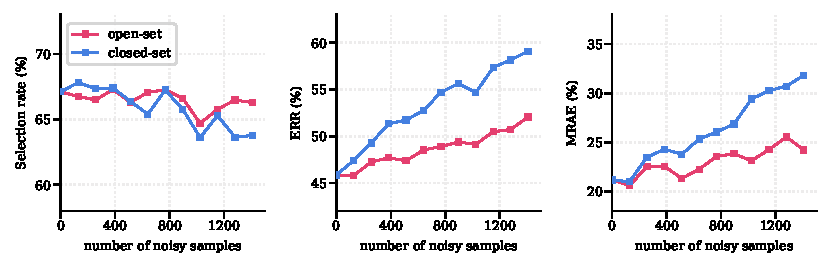
\includegraphics[width=\textwidth]{imgs/disruptive_analysis_wide_neurips.pdf}}
\caption{
\textbf{Closed-set/open-set noise analysis} displays the selection, ERR and MRAE
when closed-set or open-set noisy samples are injected into the clean dataset.
The experiments are based on IMDB-Clean-B.
% TODO: if this figure is relocated to Section 2, rename it
}
\vskip -0.3in
\label{fig:disruptive_analysis}
\end{center}
\end{figure*}



\subsection{Closed-Set versus Open-Set Noise}\label{subsec:disruptive_anomaly_noise}
To explore the impact of closed-set and open-set noisy samples, as depicted in Fig.~\ref{fig:fragment_motivation}(b) in the main manuscript, we conducted an analysis of Selection rate, ERR, and MRAE performance while gradually introducing closed-set and open-set noisy samples into the IMDB-Clean-B dataset.
Our study employs the IMDB-Clean-B dataset, comprising a fixed set of clean samples that represent 40\% of the total dataset, alongside varying amounts of noisy samples. 
These noisy samples are classified into two distinct categories: closed-set and open-set noise \citep{wei2021open, wan2024unlocking}. 
For example, consider an example with 4 fragments, whose contrastive fragment pairs are $\{(1, 3), (2, 4)\}$.
When training a feature extractor on binary classification between fragment 1 and 3, noisy sample whose ground truth fragment id is either 2 or 4 but mislabeled as fragment id of either 1 or 3 is an open-set noisy sample.
On the other hand, a noisy sample whose ground truth fragment id is 1 but mislabeled as 3 (and vice versa) is a closed-set noisy sample.
% The classification is determined by comparing their fragment ids, which incorporate the noisy label ($y$), with those containing the ground-truth label ($y^\text{gt}$).

% To provide further clarification, let's consider an example with 4 fragments, whose contrasting fragment pairs are $\{(1, 3), (2, 4)\}$: a sample with a ground-truth label has a fragment id of 1, but the noisy label has an assigned fragment id of 3, signifying a contrasting pair. 
% In such cases, we designate it as a closed-set noise sample. Conversely, if a sample with a ground-truth label has an assigned fragment id of 1, and the noisy label's assigned fragment id is either 2 or 4, which does not form a contrasting pair, we classify it as an open-set noise sample.
% Note that the notion of closed-set and open-set described in the paper is consistent with previous works \citep{wei2021open, wan2024unlocking}

Fig.~\ref{fig:disruptive_analysis} demonstrates that closed-set noisy samples have a considerably more adverse impact on ERR and MRAE compared to open-set noisy samples. 
Our contrastive fragment pair-based learning approach is advantageous in this regard, as it introduces open-set noisy samples in lieu of many closed-set noisy samples, thereby facilitating learning with reduced interference.
% This suggests that fragmenting and pairing noisy datasets can offer benefits in minimizing the disruption caused by noisy samples.

% \clearpage

\subsection{Analysis of Samples on the Bounday versus Center of Fragments}\label{subsec:boundary_center}
Table~\ref{tab:anal_boundary_centre} presents a comparative analysis of the selection rate and error reduction rate (ERR) between samples located at the boundary and the center of fragments across eight experimental configurations. 
The results indicate an average difference of 2.29\% in selection rates and 2.43\% in ERR between the two groups. 
These findings substantiate the robustness of ConFrag's sample selection process, demonstrating consistent performance irrespective of the sample's positional location within the fragment.

\begin{table*}[t]
    \centering
    \caption{Difference of selection rate and ERR between the samples at the boundary and center of fragments}
    \begin{small}
    \begin{tabular}{lcccc}
    \toprule
    \multicolumn{5}{c}{\textbf{Selection rate}} \\
    \midrule
    \textbf{} & \textbf{20\%} & \textbf{40\%} & \textbf{60\%} & \textbf{80\%} \\
    \midrule
    \textbf{boundary} & 79.55\% & 65.31\% & 55.98\% & 65.96\% \\
    \textbf{center} & 80.18\% & 66.86\% & 54.64\% & 61.16\% \\
    \textbf{difference} & 0.63\% & 1.55\% & 1.34\% & 4.80\% \\
    \midrule
    \multicolumn{5}{c}{\textbf{ERR}} \\
    \midrule
    \textbf{boundary} & 31.90\% & 39.01\% & 55.44\% & 82.26\% \\
    \textbf{center} & 30.16\% & 36.63\% & 50.42\% & 82.91\% \\
    \textbf{difference} & 1.74\% & 2.38\% & 5.02\% & 0.65\% \\
    \bottomrule
    \end{tabular}
    \end{small}
    \label{tab:anal_boundary_centre}
\end{table*}


\begin{comment}
\begin{figure}[t]
\begin{center}
% \vskip -0.32in
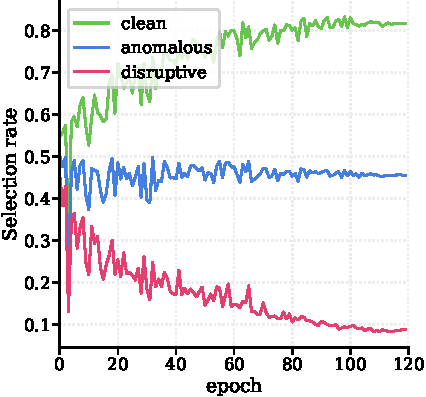
\includegraphics[width=0.4\columnwidth]{imgs/disruptive_anomaly.pdf}
\caption{\textbf{Clean/Open-set noise/Closed-set noise sample selection ratio}. 
The analysis is conducted on IMDB-Clean-B with symmetric 40\% noise.
}
\label{fig:disruptive_anomaly}
\end{center}
\end{figure}

\subsection{Selection Ratio Analysis based on Noise Types}\label{subsec:selection_ratio_noise_types}
In Fig.~\ref{fig:disruptive_anomaly}, we delineate the selected samples by FragSel on IMDB-Clean-B with symmetric 40\% noise.
Each selection ratio is calculated as, $$ \text{selection ratio} = \frac{\text{\# selected}}{\text{total}}.$$
% where the `selected number' and `total' are one of clean/open-set noise/closed-set noise, respectively.
As training progresses, FragSel select clean sample more frequently, while the selection ratio of closed-set noise decays.
%We can see that FragSel has a high clean sample selection ratio that improves with training, open-set noisy samples, and closed-set noisy samples, which decay as training progresses.
As a result, FragSel samples a higher-quality dataset as the training progresses.

% the number of samples selected (clean/anomaly/disruptive) by FragSel divided by the total number (clean/anomaly/disruptive) of samples in the dataset.
% analyze how the ratio of selected clean/anomaly/disruptive samples changes compared to the original dataset by using our method.
% In Fig.~\ref{fig:feature_space_depict}, we show a detailed or zoomed visualization of the representation space by comparing the 
% trained penultimate features of all the fragments, just two neighboring fragments trained separately, and the two most distant fragments in the label space (\ie contrasting features) also trained separately. 
% We can qualitatively verify the advantage of contrasting fragmentation on training distinct features compared to the neighboring and ``all group'' trained fragments.

% \begin{figure}[t]
% \begin{center}
% \centerline{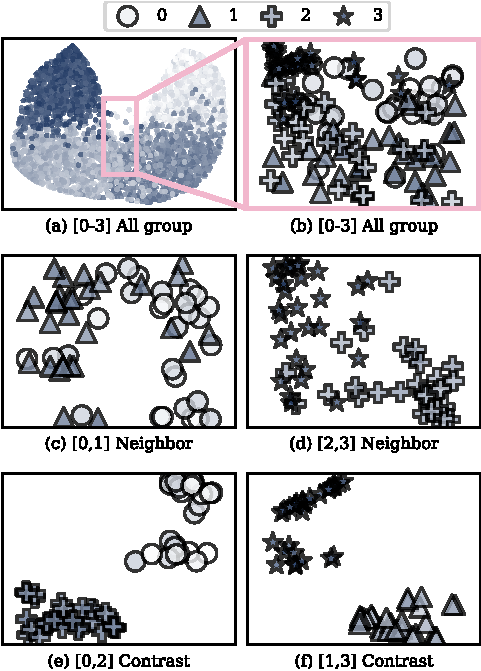
\includegraphics[width=\columnwidth]{imgs/zoomin_fragment_tsne.pdf}}
% \caption{\textbf{Detailed Representation Depiction}. A detailed comparison of the contrasting fragment's effects via visualization of the penultimate feature
% of the discriminator using t-SNE~\cite{maaten08tsne}.
% (a) the features of all the fragments trained together.
% (b) an enlarged picture of the four fragments in the box from (a).
% (c)-(d) the neighboring fragments trained together.
% (e)-(f) the contrasting fragments trained together.
% }
% \label{fig:feature_space_depict}
% \end{center}
% \vskip -0.3in
% \end{figure}
\end{comment}

% \begin{table}[t]
%     \begin{center}
%     \begin{small}
%     \setlength{\tabcolsep}{4.2pt}
%     \begin{tabular}{lccccccccc}
%         \toprule
%         \multicolumn{7}{c}{ablation and combinations}&\multicolumn{3}{c}{IMDB-Clean-B}
%         \\\cmidrule(lr){1-7} \cmidrule(lr){8-10}
%         & & & & & & & \multicolumn{1}{c}{symmetric}    &\multicolumn{2}{c}{Gaussian} \\
%         %\midrule
%         loss & backbone & pred & repr & jitter & C-Mixup & Co-teaching & 40 & 30 & 50   \\
%         \midrule
%         % Best Baseline & 27.52 & 21.90 & 43.35 & & & & & & &\\
%         % \specialrule{0.7pt}{1pt}{1pt}
%         MSE \& MSE & ResNet-18 &  \checkmark & \checkmark & & &                        & 18.35 & 20.81 & 41.81  \\
%         MSE \& MSE & ResNet-18 &  \checkmark & \checkmark & \checkmark & &             &  & & \\
%         \midrule
%         CE \& MSE  & ResNet-18 &  \checkmark  &  & & &                                 & 23.13 & 22.54 & 46.65  \\
%         CE \& MSE  & ResNet-18 &              & \checkmark &  & &                      & 21.90 & 22.02 & 45.03  \\
%         CE \& MSE  & ResNet-18 &  \checkmark  & \checkmark & & &                       & 18.90 & 21.77 & 39.78  \\
%         % CE \& MSE  & ResNet-18 &  \checkmark  &  & \checkmark & &                      & 12.59 & 14.02 & 31.15  \\
%         % CE \& MSE  & ResNet-18 &              & \checkmark & \checkmark & &            & 12.34 & 16.90 & 36.51  \\
%         CE \& MSE  & ResNet-18 &  \checkmark  & \checkmark & \checkmark & &            & 10.53 & 16.02 & 30.80  \\
%         CE \& MSE  & ResNet-34 &  \checkmark  & \checkmark & \checkmark & &            & 13.44 & 16.06 & 31.00  \\
%         CE \& MSE  & ResNet-18 &  \checkmark  & \checkmark & \checkmark & \checkmark & & 7.59 & 11.24 & 29.23  \\
%         CE \& MSE  & ResNet-18 &  \checkmark  & \checkmark & \checkmark & & \checkmark & 9.13 & 14.61 & 35.92  \\
%         \midrule
%         SCE \& MSE & ResNet-18 &  \checkmark & & & &                                   & 18.22 & 20.84 & 40.57  \\
%         SCE \& MSE & ResNet-18 &  & \checkmark & & &                                   & 17.83 & 20.92 & 39.29  \\
%         SCE \& MSE & ResNet-18 &  \checkmark & \checkmark & & &                        & 18.37 & 20.80 & 38.10  \\
%         SCE \& MSE & ResNet-18 &  \checkmark & \checkmark & \checkmark & &             & 16.84 & 20.07 & 38.18  \\
%         SCE \& MSE & ResNet-34 &  \checkmark & \checkmark & \checkmark & &             & 14.97 & 18.95 & 36.12   \\
%         SCE \& MSE & ResNet-18 &  \checkmark & \checkmark & \checkmark & \checkmark &  & 15.85 & 16.27 & 36.42   \\
%         SCE \& MSE & ResNet-18 &  \checkmark & \checkmark & \checkmark & & \checkmark  & 13.19 & 18.32 & 41.02  \\
%         \bottomrule
%     \end{tabular}
%     \end{small}
%     \end{center}
%     \caption{\textbf{Ablation and Combination Analysis.} %Three different ablations and two combinations with existing noisy techniques are studied. 
%     % The Best Baseline enlists the best MRAE for each noise type from the main manuscript for reference.
%     The values are mean relative absolute error to the noise-free model on the IMDB-Clean-B~\citep{rothe18imdb} dataset, and lower values indicate better performances. 
%     }
%     \label{tab:ablation}
% \end{table}
\begin{comment}
\begin{table}[t]
    \begin{center}
    \begin{small}
    \setlength{\tabcolsep}{4.2pt}
    \caption{\textbf{Ablation and Combination Analysis.} %Three different ablations and two combinations with existing noisy techniques are studied. 
    % The Best Baseline enlists the best MRAE for each noise type from the main manuscript for reference.
    The values are mean relative absolute error to the noise-free trained model on the IMDB-Clean-B~\citep{rothe18imdb} dataset, and lower values indicate better performances. 
    }
    \label{tab:ablation}
    \begin{tabular}{lccccccccc}
        \toprule
        \multicolumn{5}{c}{ablation and combinations}&\multicolumn{3}{c}{IMDB-Clean-B}
        \\\cmidrule(lr){1-5} \cmidrule(lr){6-8}
        & & & & & \multicolumn{1}{c}{symmetric}    &\multicolumn{2}{c}{Gaussian} \\
        %\midrule
        loss & backbone & jitter & C-Mixup & Co-teaching & 40 & 30 & 50   \\
        % \midrule
        % % Best Baseline & 27.52 & 21.90 & 43.35 & & & & & & &\\
        % % \specialrule{0.7pt}{1pt}{1pt}
        % MSE \& MSE & ResNet-18 & & &                        & 22.37 & 21.28 & 45.15  \\
        % MSE \& MSE & ResNet-18 & \checkmark & &             & 22.22 & 24.42 & 43.31 \\
        \midrule
        % CE \& MSE  & ResNet-18 &  \checkmark  &  & & &                                 & 23.13 & 22.54 & 46.65  \\
        % CE \& MSE  & ResNet-18 &              & \checkmark &  & &                      & 21.90 & 22.02 & 45.03  \\
        CE \& MSE  & ResNet-18 & & &                       & 18.90 & 21.77 & 39.78  \\
        CE \& MSE  & ResNet-18 & \checkmark & &            & 10.53 & 16.02 & 30.80  \\
        CE \& MSE  & ResNet-34 & \checkmark & &            & 13.44 & 16.06 & 31.00  \\
        CE \& MSE  & ResNet-18 & \checkmark & \checkmark & & 7.59 & 11.24 & 29.23  \\
        CE \& MSE  & ResNet-18 & \checkmark & & \checkmark & 9.13 & 14.61 & 35.92  \\
        \midrule
        % SCE \& MSE & ResNet-18 &  \checkmark & & & &                                   & 18.22 & 20.84 & 40.57  \\
        % SCE \& MSE & ResNet-18 &  & \checkmark & & &                                   & 17.83 & 20.92 & 39.29  \\
        SCE \& MSE & ResNet-18 & & &                        & 18.37 & 20.80 & 38.10  \\
        SCE \& MSE & ResNet-18 & \checkmark & &             & 16.84 & 20.07 & 38.18  \\
        SCE \& MSE & ResNet-34 & \checkmark & &             & 14.97 & 18.95 & 36.12   \\
        SCE \& MSE & ResNet-18 & \checkmark & \checkmark &  & 15.85 & 16.27 & 36.42   \\
        SCE \& MSE & ResNet-18 & \checkmark & & \checkmark  & 13.19 & 18.32 & 41.02  \\
        \bottomrule
    \end{tabular}
    \end{small}
    \end{center}
\end{table}
\end{comment}

\begin{table}[t]
    \begin{center}
    \begin{small}
    \setlength{\tabcolsep}{4.2pt}
    \caption{\textbf{Ablation and Combination Analysis.} %Three different ablations and two combinations with existing noisy techniques are studied. 
    % The Best Baseline enlists the best MRAE for each noise type from the main manuscript for reference.
    The values are mean relative absolute error to the noise-free trained model on the IMDB-Clean-B~\citep{lin2021imdbclean} dataset, and lower values indicate better performances. 
    The results are the mean of three random seed experiments.
    }
    \label{tab:ablation}
    \begin{tabular}{lcccccc}
        \toprule
        \multicolumn{4}{c}{ablation and combinations}&\multicolumn{3}{c}{IMDB-Clean-B}
        \\\cmidrule(lr){1-4} \cmidrule(lr){5-7}
        & & & & \multicolumn{1}{c}{symmetric}    &\multicolumn{2}{c}{Gaussian} \\
        %\midrule
        feat. ext. loss & backbone & jitter & Co-teaching & 40 & 30 & 50   \\
        % \midrule
        % % Best Baseline & 27.52 & 21.90 & 43.35 & & & & & & &\\
        % % \specialrule{0.7pt}{1pt}{1pt}
        % MSE \& MSE & ResNet-18 & & &                        & 22.37 & 21.28 & 45.15  \\
        % MSE \& MSE & ResNet-18 & \checkmark & &             & 22.22 & 24.42 & 43.31 \\
        \midrule
        % CE \& MSE  & ResNet-18 &  \checkmark  &  & & &                                 & 23.13 & 22.54 & 46.65  \\
        % CE \& MSE  & ResNet-18 &              & \checkmark &  & &                      & 21.90 & 22.02 & 45.03  \\
        CE  & ResNet-18 & &                        & 18.90 & 21.77 & 39.78  \\
        CE  & ResNet-18 & \checkmark &             & 12.64 & 15.70 & 33.36  \\
        CE  & ResNet-34 & \checkmark &             & 13.44 & 16.06 & 31.00  \\
        %CE  & ResNet-18 & \checkmark & \checkmark & & 7.59 & 11.24 & 29.23  \\
        CE  & ResNet-18 & \checkmark &  \checkmark & 9.45 & 14.87 & 35.88  \\
        \midrule
        % SCE \& MSE & ResNet-18 &  \checkmark & & & &                                   & 18.22 & 20.84 & 40.57  \\
        % SCE \& MSE & ResNet-18 &  & \checkmark & & &                                   & 17.83 & 20.92 & 39.29  \\
        SCE & ResNet-18 &  &                        & 18.37 & 20.80 & 38.10  \\
        SCE & ResNet-18 & \checkmark &              & 16.84 & 20.07 & 38.18  \\
        SCE & ResNet-34 & \checkmark &              & 14.97 & 18.95 & 36.12   \\
        %SCE & ResNet-18 & \checkmark & \checkmark &  & 15.85 & 16.27 & 36.42   \\
        SCE & ResNet-18 & \checkmark &  \checkmark  & 13.19 & 18.32 & 41.02  \\
        \bottomrule
    \end{tabular}
    \end{small}
    \end{center}
\end{table}

\begin{comment}
\begin{table}[t]
    \begin{center}
    \begin{small}
    \setlength{\tabcolsep}{4.2pt}
    \caption{\textbf{Ablation of Mixture of Neighboring Fragments.}
    The values are mean relative absolute error to the noise-free model on the IMDB-Clean-B~\citep{rothe18imdb} dataset, and lower values indicate better performances.
    }
    \label{tab:ablation_mnf}

    \begin{tabular}{cccccc}
        \toprule
        \multicolumn{3}{c}{ablation}&\multicolumn{3}{c}{IMDB-Clean-B}
        \\\cmidrule(lr){1-3} \cmidrule(lr){4-6}
        & & & \multicolumn{1}{c}{symmetric}    &\multicolumn{2}{c}{Gaussian} \\
        %\midrule
        $\alpha_f^\text{self}$ & $\alpha_f^\text{ngb}$ & $\mathcal{S}$ & 40 & 30 & 50\\
        \midrule
        % \specialrule{0.7pt}{1pt}{1pt}
        \checkmark &            & $\mathcal{S}^p\cup \mathcal{S}^r$  & 13.66 & 15.90 & 32.95 \\
                   & \checkmark & $\mathcal{S}^p\cup \mathcal{S}^r$  & 19.84 & 24.14 & 42.63 \\
        % \checkmark & \checkmark & $\mathcal{S}^p$                    & 23.13 & 22.54 & 46.65 \\ % no jit
        \checkmark & \checkmark & $\mathcal{S}^p$                    & 12.59 & 14.02 & 31.15 \\
        % \checkmark & \checkmark & $\mathcal{S}^r$                    & 21.90 & 22.02 & 45.03 \\ % no jit
        \checkmark & \checkmark & $\mathcal{S}^r$                    & 12.34 & 16.90 & 36.51 \\
        \checkmark & \checkmark & $\mathcal{S}^p\cap \mathcal{S}^r$  & 11.87 & 14.76 & 34.03 \\
        \checkmark & \checkmark & $\mathcal{S}^p\cup \mathcal{S}^r$  & 10.53 & 16.02 & 30.80 \\

        \bottomrule
    \end{tabular}
    \end{small}
    \end{center}
\end{table}
\end{comment}


\subsection{Ablation \& Combination Analysis}\label{subsec:ablation}
In Table~\ref{tab:ablation}, we present a comprehensive study comparing the performance of Cross-Entropy (CE) and Symmetric Cross Entropy (SCE)~\citep{wang19sce} losses in various ablation and combination experiments conducted on the IMDB-Clean-B dataset~\citep{lin2021imdbclean}, considering scenarios with 40\% symmetric noise and two variations of Gaussian random noise, each having a maximum standard deviation of 30 and 50.

% In the first ablation experiment, we utilize a regression feature extractor trained solely using the Mean Squared Error (MSE) loss. 
% While this approach performs reasonably well in isolation, it falls slightly short in achieving discriminative feature extraction performance.

% Subsequently, we perform ablations involving prediction and representation features along with jittering regularization. 
% The results clearly demonstrate the benefits of including both prediction and representation features. 
Firstly, we illustrate the impact of jittering regularization through ablation on each of the losses.
Notably, jittering regularization emerges as a crucial component of ConFrag's performance, preventing the model from overfitting to the noisy labels.

% The next ablation experiment entails replacing the ResNet-18 architecture with ResNet-34.
The next ablation experiment entails replacing the ResNet-18 architecture of the feature extractors with ResNet-34.
The performance is enhanced when trained with SCE but decreases when trained with just CE.
This suggests that ConFrag could potentially benefit from a more powerful architecture, but it is not a necessity.

A significant advantage of ConFrag lies in its compatibility with other approaches. 
% We showcase its performance when combined with two additional techniques: C-Mixup~\citep{yao22cmixup} and Co-teaching~\citep{han18coteaching}, which are also employed by CNLCU and Co-Selfie in our baseline. 
We showcase its performance when combined with an additional technique: Co-teaching~\citep{han18coteaching}, which is also employed by CNLCU and Co-Selfie in our baseline.
Co-teaching involves training the regression model while heuristically assuming that 25\% of the original noise still exists in the data (\eg 40\% original noise implies an assumption of 10\% noise during Co-teaching regression). 
% Additionally, we report the results of combining C-Mixup with our regression model. 
Empirical observations reveal that Co-teaching consistently provides significant benefits. %, while the impact of C-Mixup on performance varies depending on the scenario, but it overall performs best when used with CE.

Upon comparing CE and SCE for feature extractor training loss, we observe that CE, when combined with jitter regularization, synergizes better to exhibit much stronger performance compared to SCE.

% \begin{figure}[t]
% \begin{center}
% \centerline{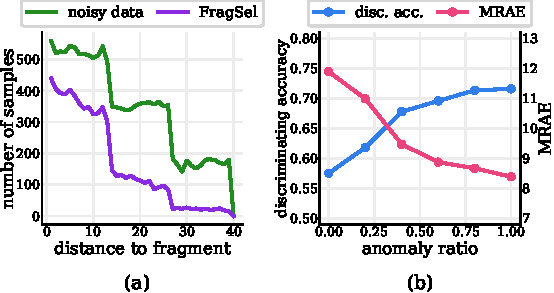
\includegraphics[width=\columnwidth]{imgs/anomaly_analysis.pdf}}
% \caption{\textbf{Anomaly Analysis.}
% (a) Plots the number of data samples based on the distance between the noisy label and its ground-truth fragment.
% The green plot graphs this relation within the original noisy dataset samples, and the purple plot graphs the FragSel selected samples.
% (b) The blue plot displays the discrimination (classification) accuracy between models trained with different anomaly ratios and 
% the corresponding regression MRAE as the red plot.
% The experiments are performed on IMDB-clean-B with a noise rate fixed to 0.4.
% }
% \label{fig:anomaly_analysis}
% \end{center}
% \vskip -0.3in
% \end{figure}


% \subsection{Anomaly Analysis}\label{subsec:anomaly}
% After contrasting fragmentation, the severity of the noise in each sample can be measured by the distance between the sample's ground-truth (clean) label, $y^c$ and 
% its assigned fragmentation based on the noisy label, $\tilde{y}^d$.
% In Fig.~\ref{fig:anomaly_analysis} (a), the aforementioned distance per sample is compared between all the noisy dataset samples and 
% the samples selected by FragSel.
% The result shows that FragSel is apt at filtering distant samples, preventing highly noisy samples from disturbing the learning.

% In Fig. 2 of the main manuscript, we categorized the noisy samples into \textit{anomalies} and \textit{disruptive samples}.
% We define the anomalies as the samples with ground-truth labels that do not belong in the assigned contrasting fragment (\eg ground-truth, $y^d=0$ is wrongly labeled as $\tilde{y}^d=1$ in contrasting fragment $[1,3]$) 
% and the disruptive samples as those that are wrongly assigned to one of the labels within the contrasting fragment %assigned included in the opposite fragment due to the noise.
% (\eg ground-truth, $y^d=1$ is wrongly labeled as $\tilde{y}^d=3$ in contrasting fragment $[1,3]$).

% In Fig.~\ref{fig:anomaly_analysis} (b), we show the effects of anomalies and disruptive samples by comparing the performance of 
% discriminative models and the regression MRAEs at different anomaly to disruption ratios with a fixed noise rate.
% It is observed that the accuracy of the discriminative model improves as more anomaly samples (or less disruptive samples) are included,
% and eventually leading to a better performance of the regression MRAE.

% In IMDB-clean-B with 0.4 symmetric noise rate, 
% We measure the aforementioned distance at each sample and plot the number of samples to distance relation.
% The total noisy dataset and samples selected by FragSel are compared.

\begin{table}[t]
    \begin{center}
    \begin{small}
    \setlength{\tabcolsep}{4.2pt}
    \caption{\textbf{Discretized Baseline Analysis.} Mean Relative Absolute Error to the noise-free model of discretized versions of strongly performing models on the IMDB-Clean-B~\citep{lin2021imdbclean} dataset. 
    Lower is better. 
    }
    \label{tab:discrete}

    \begin{tabular}{lccc}
        \toprule
        &\multicolumn{3}{c}{IMDB-Clean-B}
        \\\cmidrule(lr){2-4}
        &\multicolumn{1}{c}{symmetric}    &\multicolumn{2}{c}{Gaussian} \\
        %\midrule
        noise rate (\%)  & 40 & 30 & 50 \\
        \midrule
        % Vanilla            & & &\\
        % \specialrule{0.1pt}{1pt}{1pt}
        CNLCU-S-D~\citep{xia22} & 55.71 & 64.71 & 79.59 \\
        CNLCU-S-D + mixup~\citep{xia22} & 55.14 & 67.17 & 81.32 \\
        CNLCU-H-D~\citep{xia22} & 37.76 & 51.36  & 76.40 \\
        CNLCU-H-D + mixup~\citep{xia22} & 65.32 & 67.31 & 84.22 \\
        Sigua-D~\citep{han20sigua} & 56.17 & 61.67 & 66.08 \\
        Sigua-D + mixup~\citep{han20sigua} & 33.55 & 29.33 & 49.44 \\
        BMM-D~\citep{arazo19} & 33.86 & 30.27 & 50.05 \\
        MD-DYR-SH-D~\citep{arazo19} & 33.89 & 31.18 & 51.23 \\
        CRUST-D~\citep{mirzasoleiman20crust} & 33.86 & 30.27 & 50.47\\
        CRUST-D + mixup~\citep{mirzasoleiman20crust} & 32.33 & 30.50 & 50.27 \\
        Selfie-D~\citep{song19b} & 31.50 & 24.86 & 47.46 \\
        Selfie-D + mixup~\citep{song19b} & 35.33 & 28.02  &  46.42 \\
        Co-Selfie-D~\citep{song19b} & 30.20 & 26.36 & 49.61 \\
        Co-Selfie-D + mixup~\citep{song19b} & 33.18 & 28.28 & 52.20 \\
        % DivideMix~\cite{li2020dividemix} & & & & & & & & & & & & \\
        \specialrule{0.7pt}{1pt}{1pt}
        ConFrag  (Ours) & 12.64 & 15.70 & 33.36 \\
        Co-ConFrag (Ours) & 9.45 & 14.87  & 35.88 \\
        \bottomrule
    \end{tabular}
    \end{small}
    \end{center}
\end{table}

\subsection{Discretized Baselines}\label{subsec:discrete_baselines}
In Table~\ref{tab:discrete}, we present a discretized version of several strong baselines, including Sigua~\citep{han20sigua}, CNLCU~\citep{xia22}, BMM~\citep{arazo19}, Selfie/Co-Selfie~\citep{song19b}, MD-DYR-SH~\citep{arazo19}, and CRUST~\citep{mirzasoleiman20crust}.

The discretization process aligns with our fragmentation approach used for ConFrag. We obtain selected samples at the end of every epoch to independently train the regression model. 
Additionally, we report performance with mixup~\citep{zhang18mixup}, a technique that proves beneficial for some baselines like Sigua~\citep{han20sigua}.

Notably, most baselines exhibit a deterioration in performance following discretization. 
However, Selfie/Co-Selfie~\citep{song19b} stands out as the exception, showing an improvement in performance after discretization. 
Interestingly, Sigua is the sole method that benefits from mixup~\citep{zhang18mixup} training.

\begin{figure}[t]
    \begin{center}
    \centerline{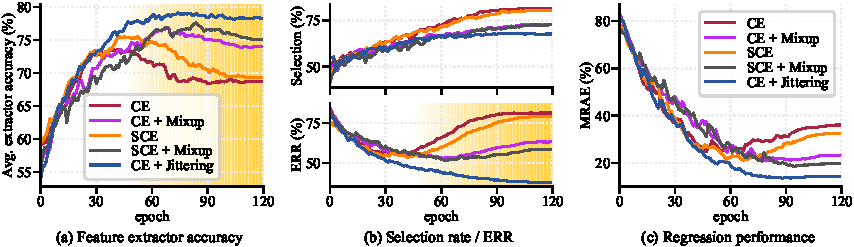
\includegraphics[width=\columnwidth]{imgs/jitter_comparison.pdf}}
    \caption{\textbf{Comparison of regularization methods}.
    Compared to other regularization methods, neighborhood jittering demonstrates superior performance in 
    (a) feature extractor test accuracy, (b) ERR, and (c) performance in regression.
    The analysis is conducted on IMDB-Clean-B with symmetric 40\% noise.
    }
    \label{fig:jitter_comparison}
    \end{center}
\end{figure}

\subsection{Comparison of Neighborhood Jittering and Other Regularization Methods}\label{subsec:jitter_comparison}
In Fig.~\ref{fig:jitter_comparison}, we compare neighborhood jittering with other regularization methods 
that can be applied to classification-based feature extractors 
(SCE with weight decay~\citep{wang19sce}, mixup~\citep{zhang18mixup}, and their combinations).
In conclusion, neighborhood jittering exhibits the strongest performance in 
feature extractor test accuracy, ERR, and MRAE, among other regularization methods. 
It is observed that ERR and MRAE improve in line with the performance of the feature extractor.

% CRUST~\citep{mirzasoleiman20crust} also performs much better in the discretized version

% \subsection{Extended ERR Analysis}\label{subsec:ERR}
% In addition to the ERR of symmetric 40\% noise IMDB-clean-B experiments on the main manuscript, we also report the ERR for the random Gaussian noise. 
% However, baselines that perform selection based on the knowledge of the noise rate in advance~\citep{xia22,han20sigua,song19b} pose a great difficulty under random 
% Gaussian noise injection. This is due to their approach to selecting a certain number of samples depending on the noise rate.
% Because the random Gaussian noise will attempt to corrupt every sample, the chance of a sample being considered noisy is very high, 
% even if the noise is within the vicinity of the original label. 
% Hence, in order to make these baselines functional and comparable, we create a \textit{soft noise rate} to be used by them for selection. 
% This is done by calculating an updated noise rate under the assumption that the noise-injected samples which fall within 12.5\% of the original ground-truth label is assumed to be clean (A range similar to our fragment size of four).
% Then to calculate the ERR, if the selected sample's label, $y$ is within $12.5\%$ of the original ground-truth label, $y^{gt}$, 
% we assume it to be a true positive prediction.
% % Otherwise, the amount correctly predicted becomes extremely small.

% Fig.~\ref{fig:gaussian_ERR} shows the results of the ERR for the random Gaussian noise experiments on IMDB-clean-B.
% We can see a noticeable gap in the ERR when there is a high amount of noise (Gaussian 50), while when the noise is relatively low (Gaussian 30),
% FragSel gradually outperforms Sigua~\citep{han20sigua} and CNLCU-H~\citep{xia22}.

\subsection{Extended Selection Rate/ERR/MRAE Comparison and Analysis}\label{subsec:ERR}
In addition to presenting the Selection rate, ERR and MRAE
for symmetric 40\%, Gaussian 30, and Gaussian 50 noise experiments on the IMDB-Clean-B dataset in the main manuscript,
we have included results for all noise types, along with additional baselines (CNLCU-H, Sigua, BMM, DY-S, AUX, Selfie, Coselfie),
in both Fig.~\ref{fig:selerr_comparison_supp1} and Fig.~\ref{fig:selerr_comparison_supp2}.

As mentioned in \S~\ref{subsec:evaluation_metrics}, the ideal scenario for selection and refurbishment methods involves achieving a high selection rate while maintaining a low ERR, 
resulting in a reduced MRAE. We examine the relationship between the selection rate, ERR, and MRAE based on Fig.~\ref{fig:selerr_comparison_supp1}(b). 
As training progresses, ConFrag and other selection methods (CNLCU-H, Sigua, BMM, DY-S) approach the ideal condition, resulting in an improving trend in MRAE. 
ConFrag, in particular, comes closest to the ideal scenario, resulting in superior MRAE performance.

The most unfavorable scenario arises when there is a low selection rate coupled with a high ERR. 
Selfie exemplifies the scenario in Fig.~\ref{fig:selerr_comparison_supp1}(b), which is connected to a relatively worse MRAE.

The scenarios of the low selection rates with low ERR and the high selection rates with high ERR can be further examined using CNLCU-H and BMM. 
CNLCU-H demonstrates superior selection quality in terms of ERR, while BMM exhibits a higher quantity in the selection rate. 
This quality/quantity trade-off is linked to the observation that CNLCU-H and BMM show similar MRAE performance in Fig.~\ref{fig:selerr_comparison_supp1}(b). 
Additionally, Fig.~\ref{fig:selerr_comparison_supp2}(a) reveals that the selection rate gap widens, while the ERR gap narrows when compared to Fig.~\ref{fig:selerr_comparison_supp1}(b). 
This is associated with BMM outperforming CNLCU-H in terms of the MRAE.

It's important to note that, rather than employing the selection rate and ERR as indicators for MRAE, 
% as discussed above, 
these metrics offer valuable insights when assessing selected or refurbished samples 
directly independent of any potential regularizing effects introduced by the underlying regression model.

In addition, upon a detailed analysis of the figures, it becomes evident that Co-ConFrag consistently achieves the lowest ERR across a wide range of noise types. 
Notably, it maintains a Selection rate of above 40\% while maintaining low ERR even in the presence of severe noise conditions, which leads to outstanding MRAE performance.

% \begin{figure}[t]
% \begin{center}
% \centerline{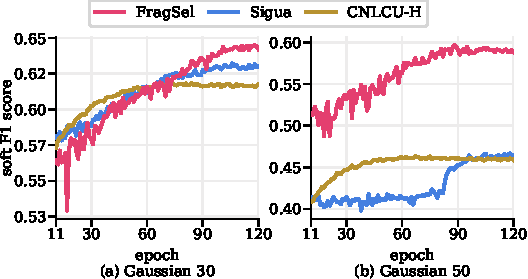
\includegraphics[width=\columnwidth]{imgs/gaussian_soft_f1_score.pdf}}
% \caption{\textbf{ERR of Gaussian random noise.}
%     (a) ERR of the Gaussian 30 noise. (b) ERR of the Gaussian 50 noise.
% }\label{fig:gaussian_ERR}
% \end{center}
% \vskip -0.3in
% \end{figure}

% \subsection{Extended Fragment Number Analysis}\label{subsec:fragment_number}
% In addition to the fragment number analysis in our main manuscript,
% Fig.~\ref{fig:split_number_shift15m} displays the performance of clean sample selection,
% and the final MRAE of the regression model on the SHIFT15M-B~\cite{kimura21shift15m} dataset.
% SHIFT15M-B mainly differs from IMDB-clean-B in that the task becomes clothing price prediction and has six times more data samples.
% We observe the selection rate (blue plot) and the average noise error (red plot)'s trend of clean selection (Fig.~\ref{fig:split_number_shift15m} 
% (a), (b)) is similar to the change in IMDB-Clean-B from the main manuscript.
% In contrast, the MRAE (Fig.~\ref{fig:split_number_shift15m} (c)) maintains a relatively low value at higher fragment numbers which
% differ from IMDB-Clean-B's increasing MRAE. This hints that exploiting the higher number of fragments could be beneficial when tackling large datasets.

\begin{figure*}[th]
\begin{center}
\centerline{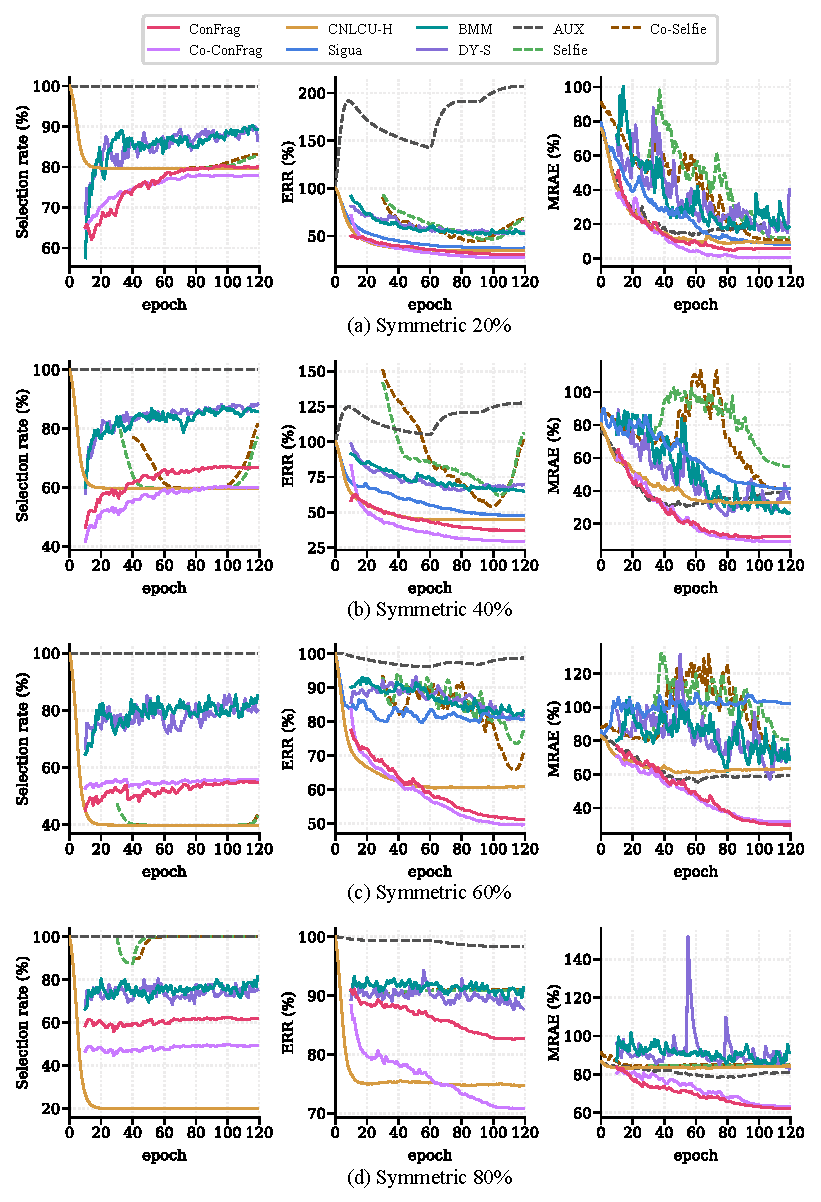
\includegraphics[width=0.75\textwidth]{imgs/selerr_comparison_supp1_neurips.pdf}}
\caption{\textbf{Selection, ERR and MRAE comparison} of ConFrag, Co-ConFrag and filtering/refurbishment baselines on IMDB-Clean-B
with symmetric 20\%(a), 40\%(b), 60\%(c) and 80\%(d) noise, repectively.
}
\label{fig:selerr_comparison_supp1}
\end{center}
\end{figure*}

\begin{figure*}[th]
\begin{center}
\centerline{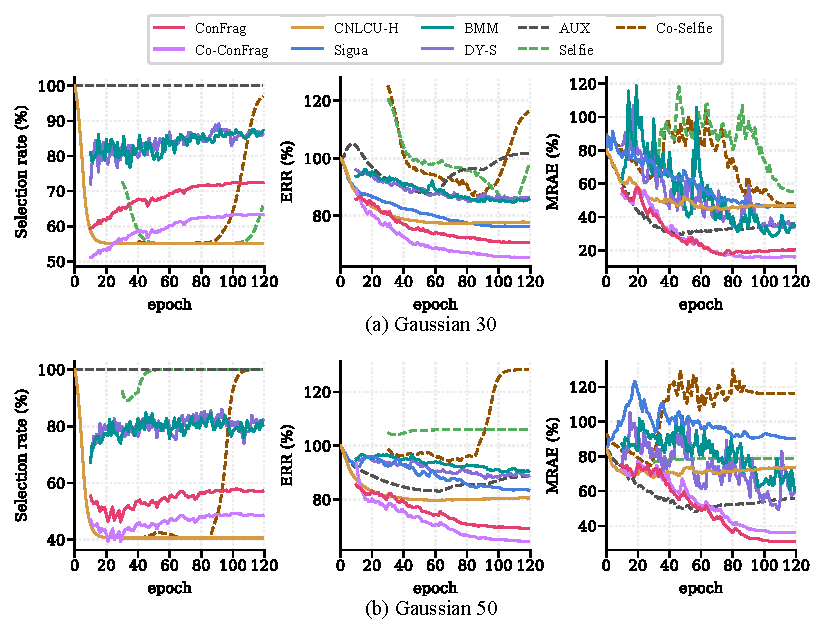
\includegraphics[width=0.75\textwidth]{imgs/selerr_comparison_supp2_neurips.pdf}}
\caption{\textbf{Selection, ERR and MRAE comparison} of ConFrag, Co-ConFrag and filtering/refurbishment baselines on IMDB-Clean-B
with Gaussian 30(a) and Gaussian 50(b) noise, repectively.
}
\label{fig:selerr_comparison_supp2}
\end{center}
\end{figure*}

\subsection{Variance Across Random Seeds}\label{subsec:variance}
In Fig.~\ref{fig:variance_analysis}, we plot the variance of three unique random seed experiments on all six noise types (symmetric 20\%/40\%/60\%/80\%, Gaussian 30/50) 
on the IMDB-Clean-B dataset. To declutter the graph, we compare it against the top two best-performing baselines under each noise type.

Tab.~\ref{tab:mrae_with_std}--\ref{tab:mrae_with_std_2} show the main experimental results of Tab.~\ref{tab:main_mrae} with standard deviation.



\subsection{Standard Mean Absolute Error}\label{subsec:mae}
In Tables~\ref{tab:main_mae}--\ref{tab:main_mae_2}, we report the standard mean absolute error (along with standard deviation) within the respective label ranges for each dataset.



\begin{figure*}[th]
\begin{center}
\centerline{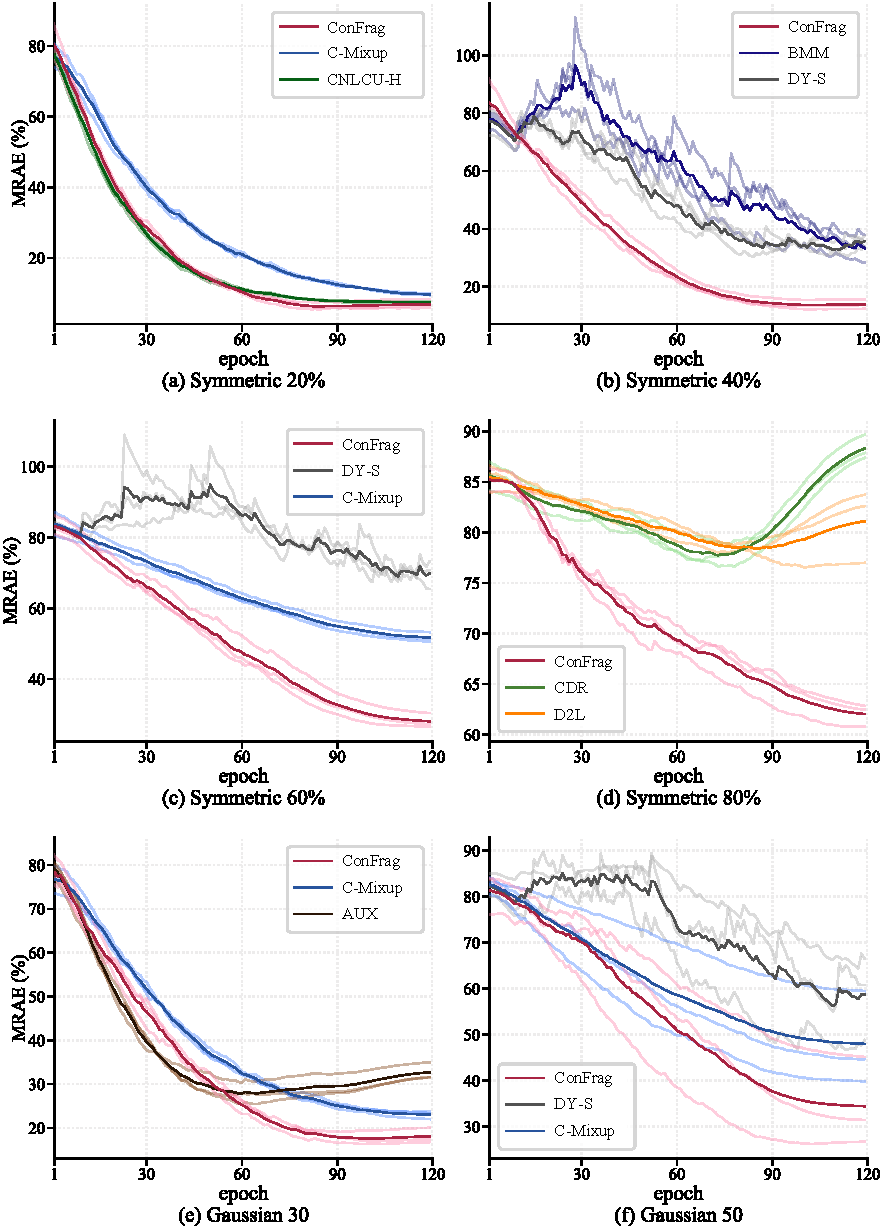
\includegraphics[width=0.75\textwidth]{imgs/variance_analysis_neurips.pdf}}
\caption{\textbf{Variance Analysis} of three unique random seed experiments on IMDB-Clean-B.  
The top two best-performing baselines under each noise type are reported.
}
\label{fig:variance_analysis}
\end{center}
\vskip -0.2in
\end{figure*}

\clearpage

\begin{table*}[t]
    \caption{\textbf{Mean Relative Absolute Error (\%)} and its standard deviation to the noise-free trained model on the AFAD-B, IMDB-Clean-B and IMDB-WIKI-B datasets.
    Lower is better. 
    A negative value indicates it performs even better than the noise-free model.
    The results are the mean of three random seed experiments.
    Number in parenthesis indicates standard deviation.
    The best and the second best methods are respectively marked in \textcolor{red}{red} and \textcolor{blue}{blue}.
    %FragSel/FragSel-R refers to classification/regression-based feature extractors.
    CNLCU-S/H, Co-Selfie, and Co-ConFrag use dual networks to teach each other as done in \citet{han18coteaching}.
    % SPR~\citep{wang22spr} fails to run for SHIFT15M-B due to excessive memory consumption.}
    }
    % \vskip -0.15in
    \begin{center}
    \begin{small}
    \setlength{\tabcolsep}{4.2pt}
    \resizebox{\columnwidth}{!}{%
    \begin{tabular}{lccccccccccccc}
        \toprule
        &\multicolumn{6}{c}{AFAD-B}         &\multicolumn{6}{c}{IMDB-Clean-B} & IMDB-WIKI-B
        \\\cmidrule(lr){2-7}\cmidrule(lr){8-13}\cmidrule(lr){14-14}
        &\multicolumn{4}{c}{symmetric}    &\multicolumn{2}{c}{Gaussian} &\multicolumn{4}{c}{symmetric} &\multicolumn{2}{c}{Gaussian} & real noise
        \\\cmidrule(lr){2-5}\cmidrule(lr){6-7}\cmidrule(lr){8-11}\cmidrule(lr){12-13}\cmidrule(lr){14-14}
        %\midrule
        noise rate  & 20 & 40 & 60 & 80 & 30 & 50 & 20 & 40 & 60 & 80 & 30 & 50 & - \\
        \midrule
        \multirow{2}{*}{Vanilla} & 9.37  & 20.27 & 30.65 & 43.09 & 28.77 & 39.03 & 16.18 & 32.05 & 53.13 & 76.35 & 26.89 & 50.28 & 00.00 \\
            & (0.72) & (0.93) & (1.15) & (45.96) & (1.57) & (4.32) & (1.60) & (0.20) & (0.93) & (1.29) & (2.45) & (9.07) & (00.00)\\
        \specialrule{0.1pt}{1pt}{1pt}
        \multirow{2}{*}{CNLCU-S} & 10.98 & 20.44 & 32.44 & 41.99 & 30.60 & 40.66 & 51.40 & 66.62 & 82.83 & 85.65 & 83.39 & 82.10 & 21.54 \\
            & (0.42) & (3.60) & (0.18) & (46.23) & (1.11) & (5.33) & (2.03) & (2.74) & (2.82) & (0.86) & (10.54) & (4.38) & (1.28)\\
        \multirow{2}{*}{CNLCU-H} & 4.63 & 16.32 & 36.01 & 44.71 & 35.68 & 43.64 & 6.84 & 31.16 & 63.08 & 82.65 & 46.53 & 65.24 & -2.93 \\
            & (0.77) & (1.51) & (3.39) & (28.95) & (3.08) & (2.79) & (0.64) & (1.29) & (2.01) & (1.65) & (5.60) & (7.16) & (0.82)\\
        \multirow{2}{*}{Sigua} & 5.96 & 21.09 & 43.33 & 49.71 & 42.52 & 46.19 & 9.82 & 46.17 & 77.59 & 85.62 & 60.97 & 77.42 & 1.96 \\
            & (1.43) & (2.15) & (2.12) & (53.69) & (3.47) & (3.85) & (0.54) & (9.52) & (2.01) & (0.94) & (19.19) & (2.07) & (1.65)\\
        \multirow{2}{*}{SPR} & 9.74 & 18.85 & 30.43 & 43.25 & 28.50 & 39.69 & 14.47 & 32.44 & 54.88 & 79.37 & 25.67 & 51.05 & -0.93 \\
            & (0.53) & (1.27) & (0.47) & (43.74) & (1.24) & (6.72) & (1.06) & (0.49) & (1.76) & (1.30) & (1.12) & (10.31) & (1.61)\\
        \multirow{2}{*}{BMM} & 5.60 & 15.00 & 39.15 & 46.41 & 30.96 & 44.00 & 8.85 & 21.54 & 55.57 & 80.40 & 24.33 & 57.21 & 17.88 \\
            & (0.68) & (1.91) & (3.16) & (44.77) & (6.89) & (2.11) & (1.53) & (2.29) & (8.88) & (3.18) & (1.49) & (16.74) & (2.05)\\
        \multirow{2}{*}{DY-S} & 6.87 & 15.56 & 32.24 & 45.72 & 24.40 & 43.41 & 10.42 & 21.90 & 49.94 & 78.16 & 24.70 & 44.56 & -3.41 \\
            & (2.22) & (3.26) & (5.14) & (33.46) & (0.68) & (4.87) & (0.96) & (1.58) & (0.26) & (0.77) & (2.23) & (10.04) & (0.86)\\
        \multirow{2}{*}{C-Mixup} & \textcolor{blue}{2.74} & 14.80 & 27.17 & 41.95 & 24.28 & 36.91 & 8.82 & 27.74 & 50.87 & 76.79 & 21.92 & 47.04 & \textcolor{blue}{-5.26} \\
            & (0.74) & (0.16) & (0.77) & (38.53) & (2.29) & (7.88) & (0.25) & (0.46) & (1.28) & (0.86) & (0.96) & (10.33) & (0.52)\\
        \multirow{2}{*}{RDI} & 10.64 & 21.80 & 39.32 & 47.07 & 37.33 & 44.41 & 16.35 & 29.33 & 55.91 & 79.92 & 25.69 & 51.35 & 1.06 \\
            & (0.41) & (0.66) & (0.76) & (49.28) & (1.51) & (4.41) & (1.09) & (1.98) & (0.60) & (0.69) & (1.75) & (12.37) & (0.67)\\
        \multirow{2}{*}{CDR} & 10.26 & 18.71 & 32.27 & 43.38 & 29.74 & 39.21 & 17.47 & 32.19 & 54.75 & 75.45 & 28.46 & 51.73 & -0.39 \\
            & (1.20) & (1.03) & (0.66) & (45.06) & (0.41) & (6.15) & (1.11) & (1.54) & (1.72) & (0.89) & (2.89) & (7.38) & (1.28)\\
        \multirow{2}{*}{D2L} & 9.43 & 20.75 & 31.25 & 44.50 & 28.86 & 40.10 & 16.94 & 33.85 & 55.54 & 76.28 & 29.30 & 52.44 & -0.66 \\
            & (0.41) & (2.51) & (0.29) & (45.37) & (1.01) & (5.73) & (1.34) & (2.21) & (0.96) & (1.00) & (3.73) & (9.20) & (0.82)\\
        \multirow{2}{*}{AUX} & 6.15 & 19.01 & 31.16 & 42.83 & 28.28 & 39.05 & 12.58 & 28.82 & 52.33 & 76.75 & 23.27 & 49.42 & -3.67 \\
            & (0.17) & (0.71) & (0.50) & (44.84) & (1.70) & (4.81) & (0.66) & (1.35) & (0.82) & (1.08) & (1.78) & (9.86) & (0.72)\\
        \multirow{2}{*}{Selfie} & 16.91 & 25.02 & 44.18 & 47.78 & 46.02 & 50.73 & 27.43 & 53.74 & 79.38 & 84.00 & 60.68 & 78.03 & 14.00 \\
            & (4.09) & (3.42) & (0.48) & (42.55) & (5.90) & (4.93) & (15.12) & (2.07) & (0.08) & (0.28) & (5.42) & (3.46) & (11.45)\\
        \multirow{2}{*}{Co-Selfie} & 14.61 & 22.95 & 39.79 & 47.72 & 41.05 & 53.00 & 23.52 & 50.07 & 67.42 & 84.25 & 52.44 & 74.73 & -0.44 \\
            & (2.66) & (1.03) & (1.33) & (35.29) & (6.05) & (15.38) & (12.18) & (11.39) & (3.08) & (0.59) & (8.15) & (6.99) & (5.19))\\
        % Superloss & 13.00 & 20.27 & 31.60 & 41.80 & 35.20 & 40.86 &	23.38 & 45.41 & 67.11 & 80.85 & 53.88 & 63.33 \\
        \multirow{2}{*}{Superloss} & 7.36 & 18.24 & 29.78 & 44.26 & 27.59 & 42.96 & 23.38 & 45.41 & 67.11 & 80.85 & 53.88 & 63.33 & -3.58 \\
            & (2.02) & (1.38) & (1.64) & (40.38) & (1.09) & (5.80) & (4.49) & (3.14) & (1.88) & (1.66) & (16.22) & (8.88) & (1.46)\\
        % OrdRegr & 31.68 & 39.85 & 49.16 & 62.54 & 54.34 & 55.60 & 89.08 & 92.00 & 105.0 & 119.5 & 92.31 & 105.6 \\
        % Crust & 44.31 & 48.41 & 49.22 & 48.66 & 51.35 & 48.25 & 75.71 & 82.29 & 86.93 & 85.55 & 84.37 & 96.07 \\
        \specialrule{0.7pt}{1pt}{1pt}
        %\textbf{FragSel-R} & 4.97 & 13.93 & 27.85 & 37.19 & 21.93 & 33.90 & 8.74 & 22.73 & 44.29 & 68.14 & 21.74 & 46.93 \\
        %\textbf{Co-FragSel-R}  & \textcolor{blue}{2.23} & 10.22 & 22.55 & 37.55 & 21.87 & 33.73 & \textcolor{blue}{2.61} & 16.06 & 40.21 & 68.00 & 18.49 & 48.79 \\
        \multirow{2}{*}{\textbf{ConFrag}}  & \textcolor{blue}{2.74} & \textcolor{blue}{8.16} & \textcolor{red}{15.91} & \textcolor{blue}{34.42} & \textcolor{blue}{17.49} & \textcolor{red}{27.31} & \textcolor{blue}{5.08} & \textcolor{blue}{12.64} & \textcolor{red}{27.26} & \textcolor{red}{61.24} & \textcolor{blue}{15.70} & \textcolor{red}{33.36} & -3.06 \\
            & (0.95) & (0.43) & (0.39) & (22.14) & (1.12) & (5.31) & (0.36) & (1.94) & (2.25) & (1.42) & (1.43) & (10.14) & (1.25)\\
        \multirow{2}{*}{\textbf{Co-ConFrag}} & \textcolor{red}{0.54} & \textcolor{red}{7.25} & \textcolor{blue}{16.65} & \textcolor{red}{33.93} & \textcolor{red}{17.43} & \textcolor{blue}{28.26} & \textcolor{red}{1.50} & \textcolor{red}{9.45} & \textcolor{blue}{28.44} & \textcolor{blue}{61.36} & \textcolor{red}{14.87} & \textcolor{blue}{35.88} & \textcolor{red}{-8.86} \\
            & (0.77) & (0.59) & (0.14) & (18.48) & (0.99) & (2.45) & (0.71) & (0.62) & (3.09) & (3.14) & (0.23) & (11.44) & (0.83)\\
        \bottomrule
    \end{tabular}
    }
    \end{small}
    \end{center}
    % \caption{\textbf{Relative Error} to noise-free model trained without noise. Smaller is better. Note that CDR~\cite{xia21cdr}, CNLCU~\cite{xia22}, Sigua~\cite{han20sigua}, Selfie~\cite{song19b} have the advantage of knowing the label noise rate.}
    \label{tab:mrae_with_std}
    \vskip -0.2in
\end{table*}

\begin{table*}[t]
    \caption{\textbf{Mean Relative Absolute Error (\%)} and its standard deviation to the noise-free trained model on the SHIFT15M-B and MSD-B datasets.
    Lower is better. A negative value indicates it performs even better than the noise-free model.
    The results are the mean of three random seed experiments.
    Number in parenthesis indicates standard deviation.
    The best and the second best methods are respectively marked in \textcolor{red}{red} and \textcolor{blue}{blue}.
    %FragSel/FragSel-R refers to classification/regression-based feature extractors.
    CNLCU-S/H, Co-Selfie, and Co-ConFrag use dual networks to teach each other as done in \citet{han18coteaching}.
    SPR~\citep{wang22spr} fails to run for SHIFT15M-B due to excessive memory consumption.}
    % \vskip -0.15in
    \begin{center}
    \begin{small}
    \setlength{\tabcolsep}{4.2pt}
    \resizebox{\columnwidth}{!}{%
    \begin{tabular}{lcccccccccccc}
        \toprule
        &\multicolumn{6}{c}{SHIFT15M-B}         &\multicolumn{6}{c}{MSD-B}
        \\\cmidrule(lr){2-7}\cmidrule(lr){8-13}
        &\multicolumn{4}{c}{symmetric}    &\multicolumn{2}{c}{Gaussian} &\multicolumn{4}{c}{symmetric} &\multicolumn{2}{c}{Gaussian}
        \\\cmidrule(lr){2-5}\cmidrule(lr){6-7}\cmidrule(lr){8-11}\cmidrule(lr){12-13} 
        %\midrule
        noise rate & 20 & 40 & 60 & 80 & 30 & 50 & 20 & 40 & 60 & 80 & 30 & 50 \\
        \midrule
        \multirow{2}{*}{Vanilla}            & 9.11 & 17.96 & 27.02 & 36.34 & 6.54 & 15.16 & 8.23 & 18.43 & 31.67 & 45.85 & 6.96 & 15.74 \\
            & (0.56) & (1.50) & (0.96) & (0.08) & (1.11) & (0.90) &	(0.18) & (2.47) & (3.51) & (0.36) & (0.65) & (3.03) \\
        \specialrule{0.1pt}{1pt}{1pt}
        \multirow{2}{*}{CNLCU-S} & 12.98 & 19.42 & 24.31 & 34.47 & 15.33 & 20.90 & 0.13 & 6.04 & 21.52 & 46.01 & 4.75 & 12.51 \\
            & (0.15) & (0.39) & (0.70) & (0.17) & (1.09) & (0.34) &	(1.18) & (0.31) & (3.61) & (1.51) & (0.92) & (1.08) \\
        \multirow{2}{*}{CNLCU-H} & 6.26 & 12.84 & 20.04 & 36.03 & 8.88 & 15.65 & 0.27 & 4.98 & 10.32 & 29.83 & 5.11 & 9.22 \\
            & (0.43) & (0.55) & (0.42) & (0.80) & (0.36) & (0.19) &	(0.19) & (0.94) & (1.46) & (1.33) & (0.31) & (0.39) \\
        \multirow{2}{*}{Sigua} & 6.94 & 14.09 & 26.08 & 37.03 & 10.32 & 17.44 & 1.29 & 7.19 & 17.35 & 50.87 & 6.80 & 12.38 \\
            & (0.13) & (0.17) & (0.29) & (2.84) & (0.77) & (0.70) &	(0.21) & (0.64) & (3.30) & (3.33) & (1.44) & (0.10) \\
        \multirow{2}{*}{SPR} &-&-&-&-&-&-& 7.07 & 18.19 & 33.39 & 45.61 & 5.01 & 15.36 \\
           & (-) & (-) & (-) & (-) & (-) & (-) & (1.30) & (1.32) & (3.17) & (2.11) & (0.31) & (2.15) \\
        \multirow{2}{*}{BMM} & 6.96 & 12.42 & 18.64 & 26.79 & 7.58 & 13.13 & 3.32 & 10.30 & 23.40 & 43.56 & 5.29 & 11.85 \\
            & (0.52) & (1.16) & (0.78) & (1.04) & (1.24) & (0.55) &	(0.64) & (1.85) & (2.31) & (1.95) & (0.63) & (0.77) \\
        \multirow{2}{*}{DY-S} & 7.11 & 11.94 & 18.85 & 29.04 & 6.90 & 13.50 & 3.39 & 8.06 & 18.65 & 35.24 & 4.77 & 9.83 \\
            & (0.25) & (0.74) & (0.10) & (1.48) & (0.97) & (0.95) &	(1.07) & (1.19) & (3.50) & (1.83) & (1.28) & (1.33) \\
        \multirow{2}{*}{C-Mixup} & 9.47 & 16.15 & 24.08 & 34.17 & 5.88 & 14.51 & 3.75 & 13.13 & 26.73 & 40.90 & 2.96 & 10.97 \\
            & (0.23) & (0.83) & (0.32) & (0.40) & (1.03) & (0.98) &	(0.83) & (2.34) & (2.16) & (2.07) & (0.17) & (0.38) \\
        \multirow{2}{*}{RDI} & 9.91 & 17.92 & 26.63 & 36.29 & 7.08 & 15.18 & 21.04 & 30.09 & 38.78 & 49.49 & 19.19 & 27.88 \\
            & (0.45) & (0.27) & (0.36) & (0.67) & (0.85) & (0.84) &	(0.09) & (0.22) & (0.98) & (1.12) & (0.69) & (1.60) \\
        \multirow{2}{*}{CDR} & 9.52 & 17.78 & 26.97 & 35.97 & 7.14 & 15.17 & 7.83 & 17.86 & 32.83 & 45.91 & 6.73 & 16.92 \\
            & (1.17) & (0.83) & (0.36) & (0.73) & (1.01) & (0.72) &	(0.91) & (3.23) & (2.36) & (0.74) & (0.49) & (1.55) \\
        \multirow{2}{*}{D2L} & 9.25 & 18.03 & 26.55 & 36.23 & 6.34 & 15.60 & 7.13 & 19.96 & 32.47 & 46.64 & 5.51 & 15.54 \\
            & (0.26) & (1.47) & (1.13) & (0.66) & (0.69) & (1.58) &	(0.37) & (1.08) & (2.21) & (2.56) & (0.76) & (2.05) \\
        \multirow{2}{*}{AUX} & 7.74 & 16.95 & 26.61 & 36.47 & 4.92 & 14.40 & 6.12 & 18.18 & 31.09 & 45.70 & 5.21 & 15.45 \\
            & (0.33) & (1.03) & (0.30) & (0.50) & (1.11) & (0.94) &	(0.88) & (1.55) & (3.07) & (1.43) & (0.28) & (1.78) \\
        \multirow{2}{*}{Selfie} & 4.84 & 10.22 & 22.28 & 38.15 & 5.51 & 11.58 & 1.43 & 8.40 & 20.24 & 45.87 & 14.37 & 24.13 \\
            & (0.77) & (0.71) & (2.82) & (0.42) & (0.97) & (0.45) &	(0.24) & (1.30) & (4.61) & (2.88) & (3.28) & (3.41) \\
        \multirow{2}{*}{Co-Selfie} & 11.53 & 16.43 & 32.08 & 39.32 & 13.45 & 22.33 & \textcolor{blue}{-0.38} & \textcolor{blue}{4.41} & \textcolor{red}{8.32} & 35.47 & 6.78 & 13.15 \\
            & (0.84) & (0.62) & (0.64) & (0.54) & (0.74) & (0.85) &	(0.12) & (0.68) & (1.40) & (0.57) & (1.70) & (1.60) \\
        % Superloss & 8.83 & 11.88 & 16.57 & 24.74 & 10.45 & 14.32 &	-0.15 & 10.68 & 23.15 & 45.55 & 4.35 & 16.36 \\
        \multirow{2}{*}{Superloss} & 5.44 & 12.26 & 23.23 & 35.24 & 5.60 & 13.28 & -0.15 & 10.68 & 23.15 & 45.55 & 4.35 & 16.36 \\
            & (1.03) & (1.48) & (1.89) & (0.28) & (1.28) & (0.67) &	(0.29) & (2.10) & (3.15) & (6.77) & (0.74) & (2.99) \\
        % OrdRegr & - & - & - & - & - & -  & 51.09 & 51.20 & 54.63 & 56.59 & 68.08 & 75.71 \\
        % Crust &-&-&-&-&-&-& 32.50 & 37.75 & 46.09 & 50.94 & 38.85 & 44.42 \\
        \specialrule{0.7pt}{1pt}{1pt}
        %\textbf{FragSel-R} & 4.18 & 9.59 & 16.21 & 25.76 & 4.96 & 10.90 & 0.77 & 5.68 & 13.63 & 30.05 & 2.79 & 6.87 \\
        %\textbf{Co-FragSel-R}  & \textcolor{blue}{1.82} & 7.67 & 14.11 & 24.11 & 3.90 & 9.64 & -0.31 & \textcolor{blue}{3.40} & 10.31 & 26.24 & \textcolor{blue}{2.18} & 6.87 \\
        \multirow{2}{*}{\textbf{ConFrag}} & \textcolor{blue}{2.46} & \textcolor{blue}{6.18} & \textcolor{red}{10.68} & \textcolor{blue}{19.04} & \textcolor{blue}{3.66} & \textcolor{red}{8.09} & 0.57 & 4.94 & 11.22 & \textcolor{blue}{23.41} & 2.39 & \textcolor{blue}{6.49} \\
            & (0.42) & (0.45) & (0.65) & (0.63) & (0.37) & (0.05) &	(0.43) & (0.34) & (1.38) & (2.00) & (0.84) & (1.90) \\
        \multirow{2}{*}{\textbf{Co-ConFrag}} & \textcolor{red}{0.85} & \textcolor{red}{5.52} & \textcolor{blue}{10.80} & \textcolor{red}{18.83} & \textcolor{red}{3.03} & \textcolor{blue}{8.70} & \textcolor{red}{-0.65} & \textcolor{red}{2.98} & \textcolor{blue}{8.66} & \textcolor{red}{20.53} & \textcolor{red}{1.73} & \textcolor{red}{6.00} \\
           & (0.31) & (0.66) & (0.43) & (0.41) & (0.94) & (0.46) &	(0.72) & (0.66) & (0.36) & (2.46) & (1.02) & (1.07) \\
        \bottomrule
    \end{tabular}
    }
    \end{small}
    \end{center}
    % \caption{\textbf{Relative Error} to noise-free model trained without noise. Smaller is better. Note that CDR~\cite{xia21cdr}, CNLCU~\cite{xia22}, Sigua~\cite{han20sigua}, Selfie~\cite{song19b} have the advantage of knowing the label noise rate.}
    \label{tab:mrae_with_std_2}
    \vskip -0.2in
\end{table*}

\begin{table*}[t]
    \caption{\textbf{Standard Mean Absolute Error} and its standard deviation to the noise-free trained model on the AFAD-B, IMDB-Clean-B and IMDB-WIKI-B datasets.
    Lower is better. 
    The results are the mean of three random seed experiments.
    Number in parenthesis indicates standard deviation.
    The best and the second best methods are respectively marked in \textcolor{red}{red} and \textcolor{blue}{blue}.
    %FragSel/FragSel-R refers to classification/regression-based feature extractors.
    CNLCU-S/H, Co-Selfie, and Co-ConFrag use dual networks to teach each other as done in \citet{han18coteaching}.
    % SPR~\citep{wang22spr} fails to run for SHIFT15M-B due to excessive memory consumption.}
    }
    \begin{center}
    \begin{small}
    \setlength{\tabcolsep}{4.2pt}
    \resizebox{\columnwidth}{!}{%
    \begin{tabular}{lccccccccccccc}
        \toprule
        &\multicolumn{6}{c}{AFAD-B}         &\multicolumn{6}{c}{IMDB-Clean-B} & IMDB-WIKI-B
        \\\cmidrule(lr){2-7}\cmidrule(lr){8-13}\cmidrule(lr){14-14}
        &\multicolumn{4}{c}{symmetric}    &\multicolumn{2}{c}{Gaussian} &\multicolumn{4}{c}{symmetric} &\multicolumn{2}{c}{Gaussian} & real noise
        \\\cmidrule(lr){2-5}\cmidrule(lr){6-7}\cmidrule(lr){8-11}\cmidrule(lr){12-13}\cmidrule(lr){14-14}
        %\midrule
        noise rate  & 20 & 40 & 60 & 80 & 30 & 50 & 20 & 40 & 60 & 80 & 30 & 50 & - \\
        \midrule
        \multirow{2}{*}{Vanilla}            & 4.75 & 5.22 & 5.68 & 6.22 & 5.59 & 6.04 & 8.11 & 9.22 & 10.70 & 12.32 & 8.86 & 10.50 & 7.23 \\
            & (0.02) & (0.03) & (0.05) & (0.06) & (0.08) & (0.18) &	(0.09) & (0.05) & (0.12) & (0.06) & (0.13) & (0.60) & (0.09)\\
        \specialrule{0.1pt}{1pt}{1pt}
        \multirow{2}{*}{CNLCU-S} & 4.82 & 5.23 & 5.75 & 6.17 & 5.67 & 6.11 & 10.57 & 11.64 & 12.77 & 12.97 & 12.81 & 12.72 & 8.78\\
            & (0.03) & (0.14) & (0.01) & (0.09) & (0.07) & (0.22) &	(0.15) & (0.20) & (0.15) & (0.04) & (0.78) & (0.25) & (0.16)\\
        \multirow{2}{*}{CNLCU-H} & 4.55 & 5.05 & 5.91 & 6.29 & 5.89 & 6.24 & 7.46 & 9.16 & 11.39 & 12.76 & 10.24 & 11.54 & 7.01\\
            & (0.05) & (0.05) & (0.16) & (0.08) & (0.15) & (0.11) &	(0.08) & (0.12) & (0.14) & (0.18) & (0.43) & (0.47) & (0.02)\\
        \multirow{2}{*}{Sigua} & 4.60 & 5.26 & 6.23 & 6.50 & 6.19 & 6.35 & 7.67 & 10.21 & 12.40 & 12.96 & 11.25 & 12.39 & 7.37\\
            & (0.07) & (0.10) & (0.07) & (0.04) & (0.17) & (0.17) &	(0.04) & (0.67) & (0.08) & (0.04) & (1.37) & (0.19) & (0.12)\\
        \multirow{2}{*}{SPR} & 4.77 & 5.16 & 5.67 & 6.22 & 5.58 & 6.07 & 8.00 & 9.25 & 10.82 & 12.53 & 8.78 & 10.55 & 7.16\\
            & (0.04) & (0.04) & (0.03) & (0.06) & (0.07) & (0.28) &	(0.09) & (0.02) & (0.08) & (0.12) & (0.05) & (0.70) & (0.03)\\
        \multirow{2}{*}{BMM} & 4.59 & 5.00 & 6.04 & 6.36 & 5.69 & 6.26 & 7.60 & 8.49 & 10.87 & 12.60 & 8.68 & 10.98 & 8.52\\
            & (0.03) & (0.09) & (0.12) & (0.06) & (0.31) & (0.09) &	(0.11) & (0.20) & (0.68) & (0.21) & (0.12) & (1.16) & (0.13)\\
        \multirow{2}{*}{DY-S} & 4.64 & 5.02 & 5.74 & 6.33 & 5.40 & 6.23 & 7.71 & 8.51 & 10.47 & 12.44 & 8.71 & 10.10 & 6.98\\
            & (0.09) & (0.12) & (0.24) & (0.16) & (0.05) & (0.20) &	(0.11) & (0.13) & (0.04) & (0.05) & (0.14) & (0.68) & (0.07)\\
        \multirow{2}{*}{C-Mixup} & \textcolor{blue}{4.46} & 4.99 & 5.52 & 6.17 & 5.40 & 5.95 & 7.60 & 8.92 & 10.54 & 12.35 & 8.52 & 10.27 & \textcolor{blue}{6.84}\\
            & (0.04) & (0.02) & (0.05) & (0.07) & (0.12) & (0.34) &	(0.06) & (0.04) & (0.06) & (0.12) & (0.04) & (0.69) & (0.04)\\
        \multirow{2}{*}{RDI} & 4.81 & 5.29 & 6.05 & 6.39 & 5.97 & 6.27 & 8.13 & 9.03 & 10.89 & 12.57 & 8.78 & 10.57 & 7.30\\
            & (0.02) & (0.04) & (0.02) & (0.02) & (0.09) & (0.18) &	(0.04) & (0.19) & (0.04) & (0.11) & (0.10) & (0.84) & (0.04) \\
        \multirow{2}{*}{CDR} & 4.79 & 5.16 & 5.75 & 6.23 & 5.64 & 6.05 & 8.20 & 9.23 & 10.81 & 12.25 & 8.97 & 10.60 & 7.20\\
            & (0.04) & (0.03) & (0.03) & (0.10) & (0.03) & (0.26) &	(0.08) & (0.16) & (0.16) & (0.02) & (0.16) & (0.48) & (0.01)\\
        \multirow{2}{*}{D2L} & 4.75 & 5.24 & 5.70 & 6.28 & 5.60 & 6.09 & 8.17 & 9.35 & 10.86 & 12.31 & 9.03 & 10.65 & 7.18\\
            & (0.03) & (0.10) & (0.03) & (0.11) & (0.03) & (0.24) &	(0.05) & (0.11) & (0.09) & (0.01) & (0.21) & (0.62) & (0.12)\\
        \multirow{2}{*}{AUX} & 4.61 & 5.17 & 5.70 & 6.20 & 5.57 & 6.04 & 7.86 & 9.00 & 10.64 & 12.35 & 8.61 & 10.44 & 6.96\\
            & (0.02) & (0.05) & (0.04) & (0.07) & (0.09) & (0.20) &	(0.01) & (0.11) & (0.11) & (0.13) & (0.13) & (0.66) & (0.05) \\
        \multirow{2}{*}{Selfie} & 5.08 & 5.43 & 6.26 & 6.42 & 6.34 & 6.55 & 8.90 & 10.74 & 12.53 & 12.85 & 11.22 & 12.43 & 8.24\\
            & (0.19) & (0.16) & (0.01) & (0.01) & (0.28) & (0.23) &	(1.07) & (0.10) & (0.07) & (0.05) & (0.39) & (0.21) & (0.92)\\
        \multirow{2}{*}{Co-Selfie} & 4.98 & 5.34 & 6.07 & 6.42 & 6.13 & 6.65 & 8.63 & 10.48 & 11.69 & 12.87 & 10.65 & 12.20 & 7.20\\
            & (0.13) & (0.06) & (0.08) & (0.08) & (0.28) & (0.68) &	(0.88) & (0.84) & (0.19) & (0.03) & (0.61) & (0.45) & (0.46)\\
        \multirow{2}{*}{Superloss} & 4.66 & 5.14 & 5.64 & 6.27 & 5.54 & 6.21 & 8.62 & 10.16 & 11.67 & 12.63 & 10.75 & 11.41 & 6.97\\
            & (0.07) & (0.05) & (0.05) & (0.05) & (0.05) & (0.25) &	(0.27) & (0.25) & (0.19) & (0.15) & (1.14) & (0.57) & (0.05)\\
        
        % OrdRegr & 5.72 & 6.07 & 6.48 & 7.06 & 6.70 & 6.76 & 13.21 & 13.41 & 14.32 & 15.33 & 13.43 & 14.35 \\
        % CRUST & 6.27 & 6.45 & 6.48 & 6.46 & 6.58 & 6.44 & 12.27 & 12.73 & 13.06 & 12.96 & 12.88 & 13.69 \\
        % DivideMix~\citep{li2020dividemix} & & & & & & & & & & & & \\
        \specialrule{0.7pt}{1pt}{1pt}
        %\textbf{FragSel-R} & 4.56 & 4.95 & 5.55 & 5.96 & 5.30 & 5.82 & 7.59 & 8.57 & 10.08 & 11.74 & 8.50 & 10.26 \\
        %\textbf{Co-FragSel-R} & \textcolor{blue}{4.44} & 4.79 & 5.32 & 5.97 & \textcolor{blue}{5.29} & 5.81 & \textcolor{blue}{7.17} & 8.11 & 9.79 & 11.73 & 8.28 & 10.39 \\
        \multirow{2}{*}{\textbf{ConFrag}} & \textcolor{blue}{4.46} & \textcolor{blue}{4.70} & \textcolor{red}{5.04} & \textcolor{blue}{5.84} & \textcolor{red}{5.10} & \textcolor{red}{5.53} & \textcolor{blue}{7.34} & \textcolor{blue}{7.87} & \textcolor{red}{8.89} & \textcolor{red}{11.26} & \textcolor{blue}{8.08} & \textcolor{red}{9.31} & 7.00\\
            & (0.04) & (0.02) & (0.03) & (0.05) & (0.06) & (0.22) &	(0.04) & (0.15) & (0.12) & (0.04) & (0.07) & (0.68) & (0.13)\\
        \multirow{2}{*}{\textbf{Co-ConFrag}} & \textcolor{red}{4.37} & \textcolor{red}{4.66} & \textcolor{blue}{5.07} & \textcolor{red}{5.82} & \textcolor{red}{5.10} & \textcolor{blue}{5.57} & \textcolor{red}{7.09} & \textcolor{red}{7.64} & \textcolor{blue}{8.97} & \textcolor{blue}{11.27} & \textcolor{red}{8.02} & \textcolor{blue}{9.49} & \textcolor{red}{6.58}\\
            & (0.05) & (0.04) & (0.01) & (0.09) & (0.06) & (0.11) &	(0.08) & (0.05) & (0.20) & (0.16) & (0.05) & (0.76) & (0.06)\\
        \bottomrule
    \end{tabular}
    }
    \end{small}
    \end{center}
    % \caption{\textbf{Relative Error} to Vanilla model trained without noise. Smaller is better. Note that CDR~\citep{xia21cdr}, CNLCU~\citep{xia22}, Sigua~\citep{han20sigua}, Selfie~\citep{song19b} have the advantage of knowing the label noise rate.}
    \label{tab:main_mae}
% \vskip -0.3in
\end{table*}

\begin{table*}[t]
    \caption{\textbf{Standard Mean Absolute Error} and its standard deviation to the noise-free trained model on the SHIFT15M-B and MSD-B datasets.
    Lower is better.
    The results are the mean of three random seed experiments.
    Number in parenthesis indicates standard deviation.
    The best and the second best methods are respectively marked in \textcolor{red}{red} and \textcolor{blue}{blue}.
    %FragSel/FragSel-R refers to classification/regression-based feature extractors.
    CNLCU-S/H, Co-Selfie, and Co-ConFrag use dual networks to teach each other as done in \citet{han18coteaching}.
    SPR~\citep{wang22spr} fails to run for SHIFT15M-B due to excessive memory consumption.}
    \begin{center}
    \begin{small}
    \setlength{\tabcolsep}{4.2pt}
    \resizebox{\columnwidth}{!}{%
    \begin{tabular}{lcccccccccccc}
        \toprule
        &\multicolumn{6}{c}{SHIFT15M-B}         &\multicolumn{6}{c}{MSD-B}
        \\\cmidrule(lr){2-7}\cmidrule(lr){8-13}
        &\multicolumn{4}{c}{symmetric}    &\multicolumn{2}{c}{Gaussian} &\multicolumn{4}{c}{symmetric} &\multicolumn{2}{c}{Gaussian}
        \\\cmidrule(lr){2-5}\cmidrule(lr){6-7}\cmidrule(lr){8-11}\cmidrule(lr){12-13} 
        %\midrule
        noise rate   & 20 & 40 & 60 & 80 & 30 & 50 & 20 & 40 & 60 & 80 & 30 & 50 \\
        \midrule
        % Vanilla            & 7.47 & 8.08 & 8.70 & 9.34 & 7.30 & 7.89 & 0.5918 & 0.6475 & 0.7199 & 0.7974 & 0.5848 & 0.6328 \\
        \multirow{2}{*}{Vanilla}            & 7.47 & 8.08 & 8.70 & 9.34 & 7.30 & 7.89 & .5918 & .6475 & .7199 & .7974 & .5848 & .6328 \\
            & (0.02) & (0.07) & (0.08) & (0.04) & (0.05) & (0.08) &	(.0024) & (.0112) & (.0171) & (.0016) & (.0031) & (.0161) \\
        \specialrule{0.1pt}{1pt}{1pt}
        \multirow{2}{*}{CNLCU-S} & 7.74 & 8.18 & 8.51 & 9.21 & 7.90 & 8.28 & .5475 & .5798 & .6644 & .7983 & .5727 & .6151 \\
            & (0.03) & (0.04) & (0.01) & (0.05) & (0.04) & (0.02) &	(.0068) & (.0010) & (.0176) & (.0052) & (.0033) & (.0035) \\
        \multirow{2}{*}{CNLCU-H} & 7.28 & 7.73 & 8.22 & 9.32 & 7.46 & 7.92 & .5483 & .5740 & .6032 & .7098 & .5747 & .5972 \\
            & (0.03) & (0.04) & (0.01) & (0.05) & (0.01) & (0.03) &	(.0034) & (.0027) & (.0055) & (.0065) & (.0040) & (.0019) \\
        \multirow{2}{*}{Sigua} & 7.32 & 7.81 & 8.64 & 9.39 & 7.56 & 8.04 & .5538 & .5861 & .6416 & .8248 & .5839 & .6145 \\
            & (0.03) & (0.03) & (0.06) & (0.24) & (0.02) & (0.08) &	(.0035) & (.0024) & (.0154) & (.0150) & (.0062) & (.0026) \\
        \multirow{2}{*}{SPR} & -&-&-&-&-&-& .5854 & .6462 & .7293 & .7961 & .5741 & .6308 \\
            & (-)&(-)&(-)&(-)&(-)&(-)& (.0059) & (.0048) & (.0147) & (.0113) & (.0028) & (.0119) \\
        \multirow{2}{*}{BMM} & 7.33 & 7.70 & 8.13 & 8.68 & 7.37 & 7.75 & .5649 & .6031 & .6747 & .7849 & .5757 & .6116 \\
            & (0.03) & (0.05) & (0.03) & (0.08) & (0.06) & (0.07) &	(.0044) & (.0081) & (.0099) & (.0073) & (.0016) & (.0025) \\
        \multirow{2}{*}{DY-S} & 7.34 & 7.67 & 8.14 & 8.84 & 7.32 & 7.77 & .5653 & .5908 & .6487 & .7394 & .5728 & .6005 \\
            & (0.02) & (0.03) & (0.04) & (0.10) & (0.03) & (0.10) &	(.0072) & (.0040) & (.0164) & (.0102) & (.0045) & (.0049) \\
        \multirow{2}{*}{C-Mixup} & 7.50 & 7.95 & 8.50 & 9.19 & 7.25 & 7.84 & .5673 & .6185 & .6929 & .7704 & .5630 & .6067 \\
            & (0.03) & (0.03) & (0.03) & (0.05) & (0.04) & (0.08) &	(.0041) & (.0107) & (.0096) & (.0135) & (.0023) & (.0028) \\
        \multirow{2}{*}{RDI} & 7.53 & 8.08 & 8.67 & 9.33 & 7.33 & 7.89 & .6618 & .7113 & .7588 & .8174 & .6517 & .6992 \\
            & (0.02) & (0.02) & (0.05) & (0.03) & (0.02) & (0.08) &	(.0030) & (.0040) & (.0050) & (.0039) & (.0065) & (.0092) \\
        \multirow{2}{*}{CDR} & 7.50 & 8.07 & 8.70 & 9.31 & 7.34 & 7.89 & .5896 & .6444 & .7262 & .7978 & .5836 & .6393 \\
            & (0.05) & (0.03) & (0.05) & (0.02) & (0.04) & (0.08) &	(.0065) & (.0160) & (.0116) & (.0062) & (.0030) & (.0089) \\
        \multirow{2}{*}{D2L} & 7.48 & 8.08 & 8.67 & 9.33 & 7.28 & 7.92 & .5857 & .6559 & .7243 & .8018 & .5769 & .6317 \\
            & (0.03) & (0.07) & (0.07) & (0.01) & (0.01) & (0.13) &	(.0021) & (.0049) & (.0116) & (.0122) & (.0030) & (.0106) \\
        \multirow{2}{*}{AUX} & 7.38 & 8.01 & 8.67 & 9.35 & 7.19 & 7.83 & .5802 & .6462 & .7167 & .7966 & .5753 & .6312 \\
            & (0.01) & (0.04) & (0.04) & (0.04) & (0.04) & (0.08) &	(.0027) & (.0097) & (.0152) & (.0067) & (.0010) & (.0089) \\
        \multirow{2}{*}{Selfie} & 7.18 & 7.55 & 8.37 & 9.46 & 7.23 & 7.64 & .5546 & .5927 & .6574 & .7976 & .6253 & .6787 \\
            & (0.03) & (0.03) & (0.19) & (0.02) & (0.04) & (0.05) &	(.0020) & (.0046) & (.0230) & (.0174) & (.0190) & (.0175) \\
        \multirow{2}{*}{Co-Selfie} & 7.64 & 7.97 & 9.05 & 9.54 & 7.77 & 8.38 & \textcolor{blue}{.5447} & \textcolor{blue}{.5709} & \textcolor{red}{.5923} & .7407 & .5839 & .6187 \\
            & (0.03) & (0.01) & (0.01) & (0.01) & (0.02) & (0.08) &	(.0026) & (.0019) & (.0088) & (.0023) & (.0105) & (.0084) \\
        \multirow{2}{*}{Superloss} & 7.22 & 7.69 & 8.44 & 9.26 & 7.23 & 7.76 & .5460 & .6052 & .6733 & .7959 & .5706 & .6362 \\
            & (0.06) & (0.07) & (0.09) & (0.06) & (0.06) & (0.06) &	(.0036) & (.0104) & (.0153) & (.0405) & (.0065) & (.0140) \\
        % OrdRegr & -&-&-&-&-&-& 0.8135 & 0.8210 & 0.8597 & 0.8522 & 0.8888 & 0.9073 \\
        % CRUST & -&-&-&-&-&-& 0.7365 & 0.7674 & 0.8011 & 0.8327 & 0.7753 & 0.7965 \\
        % DivideMix~\citep{li2020dividemix} & & & & & & & & & & & & \\
        \specialrule{0.7pt}{1pt}{1pt}
        %\textbf{FragSel-R} & 7.13 & 7.51 & 7.96 & 8.61 & 7.19 & 7.60 & .5510 & .5778 & .6212 & .7110 & .5620 & .5843 \\
        %\textbf{Co-FragSel-R} & \textcolor{blue}{6.97} & 7.37 & 7.81 & 8.50 & 7.12 & 7.51 & .5451 & \textcolor{blue}{.5654} & .6031 & .6902 & \textcolor{blue}{.5587} & .5843 \\
        \multirow{2}{*}{\textbf{ConFrag}} & \textcolor{blue}{7.02} & \textcolor{blue}{7.27} & \textcolor{red}{7.58} & \textcolor{blue}{8.15} & \textcolor{blue}{7.10} & \textcolor{red}{7.40} & .5499 & .5738 & .6081 & \textcolor{blue}{.6747} & \textcolor{blue}{.5598} & \textcolor{blue}{.5822} \\
            & (0.01) & (0.02) & (0.01) & (0.03) & (0.01) & (0.04) &	(.0035) & (.0039) & (.0051) & (.0098) & (.0050) & (.0084) \\
        \multirow{2}{*}{\textbf{Co-ConFrag}} & \textcolor{red}{6.91} & \textcolor{red}{7.23} & \textcolor{blue}{7.59} & \textcolor{red}{8.14} & \textcolor{red}{7.06} & \textcolor{blue}{7.44} & \textcolor{red}{.5432} & \textcolor{red}{.5631} & \textcolor{blue}{.5941} & \textcolor{red}{.6590} & \textcolor{red}{.5562} & \textcolor{red}{.5796} \\
            & (0.01) & (0.01) & (0.01) & (0.06) & (0.04) & (0.06) &	(.0056) & (.0018) & (.0009) & (.0129) & (.0051) & (.0044) \\
        \bottomrule
    \end{tabular}
    }
    \end{small}
    \end{center}
    % \caption{\textbf{Relative Error} to Vanilla model trained without noise. Smaller is better. Note that CDR~\citep{xia21cdr}, CNLCU~\citep{xia22}, Sigua~\citep{han20sigua}, Selfie~\citep{song19b} have the advantage of knowing the label noise rate.}
    \label{tab:main_mae_2}
% \vskip -0.3in
\end{table*}




% \begin{table*}[t]
%     \caption{\textbf{Hyperparameter analysis.} Mean Relative Absolute Error to the noise-free Vanilla model on the AFAD-B, IMDB-Clean-B, SHIFT15M-B, MSD-B dataset.
%     Lower is better.
%     }\label{tab:hyperparameter_analysis}
%     \begin{center}
%     \begin{small}
%     \setlength{\tabcolsep}{4.2pt}
%     \begin{tabular}{ccc|cccc|cc|cccc|cc}
%         \toprule
%         \multicolumn{3}{c}{ }&\multicolumn{6}{c}{AFAD-B}&\multicolumn{6}{c}{IMDB-Clean-B} \\
%         \multicolumn{3}{c}{ }&\multicolumn{4}{c|}{symmetric}&\multicolumn{2}{c|}{Gaussian}&\multicolumn{4}{c|}{symmetric}&\multicolumn{2}{c}{Gaussian} \\
%         \midrule
%         % \multicolumn{3}{c}{F, K, J} & 20 & 40 & 60 & 80 & 30 & 50 & 20 & 40 & 60 & 80 & 30 & 50 \\
%         F & K & J & 20 & 40 & 60 & 80 & 30 & 50 & 20 & 40 & 60 & 80 & 30 & 50 \\
%         \midrule
%         4 & 3 & 0.90 & 4.49 & 8.39 & 18.44 & 36.70 & 20.32 & 35.65 & 6.15 & 16.39 & 38.62 & 69.24 & 18.63 & 38.02 \\
%         4 & 3 & 0.95 & 3.33 & 9.73 & 20.99 & 36.18 & 17.22 & 33.54 & 6.48 & 14.06 & 34.16 & 62.16 & 16.55 & 37.02 \\
%         4 & 3 & 1.00 & 3.64 & 14.57 & 23.13 & 40.72 & 22.37 & 35.60 & 8.33 & 21.92 & 46.00 & 69.51 & 22.19 & 44.98 \\
%         \specialrule{0.1pt}{1pt}{1pt}
%         4 & 5 & 0.90 & 2.92 & 8.62 & 16.85 & 39.82 & 21.85 & 37.85 & 5.62 & 12.75 & 39.05 & 74.65 & 16.24 & 37.39 \\
%         4 & 5 & 0.95 & 4.61 & 10.63 & 23.44 & 38.25 & 17.71 & 31.06 & 4.78 & 13.11 & 29.72 & 62.96 & 16.02 & 32.16 \\
%         4 & 5 & 1.00 & 5.64 & 18.54 & 22.46 & 41.63 & 21.71 & 36.45 & 10.03 & 22.07 & 45.15 & 71.59 & 22.44 & 46.72 \\
%         \specialrule{0.1pt}{1pt}{1pt}
%         4 & 7 & 0.90 & 4.21 & 8.44 & 15.46 & 40.16 & 20.67 & 35.67 & 5.65 & 13.69 & 39.02 & 79.04 & 17.01 & 38.72 \\
%         4 & 7 & 0.95 & 3.53 & 11.03 & 25.80 & 37.19 & 18.65 & 31.48 & 6.42 & 10.53 & 30.59 & 64.72 & 16.76 & 30.80 \\
%         4 & 7 & 1.00 & 5.31 & 13.67 & 24.92 & 42.12 & 22.75 & 35.47 & 8.91 & 22.35 & 47.40 & 72.86 & 24.07 & 46.39 \\
%         \midrule
%         6 & 3 & 0.90 & 5.85 & 11.54 & 20.17 & 35.21 & 18.75 & 35.89 & 5.89 & 17.14 & 37.05 & 69.72 & 23.23 & 40.32 \\
%         6 & 3 & 0.95 & 5.02 & 11.33 & 19.13 & 33.65 & 18.20 & 34.99 & 7.08 & 15.94 & 38.85 & 66.62 & 20.21 & 36.26 \\
%         6 & 3 & 1.00 & 9.15 & 17.48 & 26.17 & 37.61 & 24.75 & 37.51 & 10.91 & 25.03 & 47.83 & 70.14 & 25.35 & 49.06 \\
%         \specialrule{0.1pt}{1pt}{1pt}
%         6 & 5 & 0.90 & 5.87 & 12.15 & 18.95 & 35.72 & 18.19 & 33.52 & 6.18 & 14.41 & 36.78 & 71.31 & 20.90 & 42.22 \\
%         6 & 5 & 0.95 & 7.19 & 12.03 & 19.46 & 39.09 & 17.41 & 34.23 & 8.83 & 14.65 & 38.87 & 74.93 & 18.40 & 33.18 \\
%         6 & 5 & 1.00 & 8.02 & 16.65 & 29.69 & 44.85 & 23.72 & 38.44 & 11.25 & 22.84 & 49.03 & 67.84 & 24.73 & 51.82 \\
%         \specialrule{0.1pt}{1pt}{1pt}
%         6 & 7 & 0.90 & 5.47 & 13.11 & 21.39 & 37.31 & 17.22 & 33.83 & 6.95 & 16.14 & 37.41 & 72.20 & 22.95 & 41.96 \\
%         6 & 7 & 0.95 & 6.97 & 11.40 & 19.37 & 38.84 & 19.73 & 35.03 & 6.19 & 14.72 & 41.08 & 78.61 & 19.96 & 34.23 \\
%         6 & 7 & 1.00 & 8.28 & 16.06 & 29.13 & 44.07 & 24.35 & 38.04 & 11.17 & 25.36 & 50.87 & 69.74 & 24.03 & 49.43 \\
%         \midrule
%         8 & 3 & 0.90 & 5.90 & 11.93 & 22.87 & 35.99 & 20.36 & 33.60 & 7.88 & 20.11 & 42.88 & 68.66 & 23.49 & 44.33 \\
%         8 & 3 & 0.95 & 6.90 & 12.28 & 23.42 & 35.29 & 21.85 & 36.05 & 8.54 & 19.78 & 44.63 & 64.86 & 20.34 & 39.29 \\
%         8 & 3 & 1.00 & 8.71 & 17.20 & 26.99 & 38.84 & 24.01 & 38.76 & 10.85 & 25.99 & 50.11 & 72.70 & 24.97 & 46.97 \\
%         \specialrule{0.1pt}{1pt}{1pt}
%         8 & 5 & 0.90 & 5.17 & 12.13 & 19.65 & 36.15 & 19.95 & 31.62 & 9.70 & 19.10 & 44.67 & 68.72 & 21.09 & 42.51 \\
%         8 & 5 & 0.95 & 5.86 & 10.44 & 20.89 & 35.17 & 18.99 & 32.61 & 7.52 & 19.72 & 42.30 & 63.68 & 21.41 & 39.84 \\
%         8 & 5 & 1.00 & 7.25 & 15.64 & 29.96 & 40.56 & 26.43 & 37.24 & 11.81 & 27.35 & 50.85 & 71.71 & 25.81 & 51.09 \\
%         \specialrule{0.1pt}{1pt}{1pt}
%         8 & 7 & 0.90 & 6.91 & 12.33 & 21.20 & 36.34 & 19.40 & 32.84 & 8.46 & 18.73 & 45.64 & 69.06 & 21.65 & 45.70 \\
%         8 & 7 & 0.95 & 5.81 & 12.52 & 21.98 & 36.92 & 22.01 & 34.15 & 9.03 & 18.67 & 41.60 & 64.22 & 19.53 & 38.88 \\
%         8 & 7 & 1.00 & 7.83 & 16.38 & 29.84 & 40.43 & 25.98 & 37.88 & 11.88 & 24.89 & 55.06 & 73.10 & 28.08 & 51.13 \\
%         \bottomrule
%     \end{tabular}
%     \end{small}
%     \end{center}
% \end{table*}

% \begin{table*}[t]
%     \begin{center}
%     \begin{small}
%     \setlength{\tabcolsep}{4.2pt}
%     \begin{tabular}{ccc|cccc|cc|cccc|cc}
%         \toprule
%         \multicolumn{3}{c}{ }&\multicolumn{6}{c}{SHIFT15M-B}&\multicolumn{6}{c}{MSD-B} \\
%         \multicolumn{3}{c}{ }&\multicolumn{4}{c|}{symmetric}&\multicolumn{2}{c|}{Gaussian}&\multicolumn{4}{c|}{symmetric}&\multicolumn{2}{c}{Gaussian} \\
%         \midrule
%         % \multicolumn{3}{c}{F, K, J} & 20 & 40 & 60 & 80 & 30 & 50 & 20 & 40 & 60 & 80 & 30 & 50 \\
%         F & K & J & 20 & 40 & 60 & 80 & 30 & 50 & 20 & 40 & 60 & 80 & 30 & 50 \\
%         \midrule
%         4 & 3 & 0.90 & 2.69 & 6.01 & 12.04 & 23.36 & 3.67 & 8.09 & 1.72 & 6.89 & 16.19 & 30.28 & 2.11 & 8.14 \\
%         4 & 3 & 0.95 & 2.61 & 6.13 & 11.48 & 21.95 & 4.05 & 8.14 & 0.15 & 6.34 & 16.30 & 26.84 & 1.58 & 8.07 \\
%         4 & 3 & 1.00 & 6.28 & 10.93 & 16.72 & 26.50 & 4.74 & 10.97 & 0.90 & 6.29 & 18.39 & 28.49 & 2.58 & 7.83 \\
%         \specialrule{0.1pt}{1pt}{1pt}
%         4 & 5 & 0.90 & 3.49 & 6.49 & 11.19 & 20.50 & 3.74 & 10.20 & 1.98 & 6.01 & 12.63 & 22.57 & 2.90 & 8.25 \\
%         4 & 5 & 0.95 & 3.09 & 6.19 & 10.74 & 18.73 & 4.26 & 9.17 & 0.11 & 5.11 & 12.06 & 22.14 & 2.00 & 6.75 \\
%         4 & 5 & 1.00 & 6.71 & 12.65 & 17.99 & 26.15 & 5.35 & 11.73 & 0.79 & 5.90 & 15.78 & 25.70 & 2.38 & 6.23 \\
%         \specialrule{0.1pt}{1pt}{1pt}
%         4 & 7 & 0.90 & 3.72 & 7.10 & 12.51 & 22.18 & 4.39 & 10.80 & 2.13 & 6.23 & 12.58 & 22.49 & 3.35 & 8.93 \\
%         4 & 7 & 0.95 & 3.21 & 6.39 & 11.29 & 21.14 & 4.17 & 9.25 & 0.60 & 5.26 & 11.57 & 22.60 & 2.31 & 7.11 \\
%         4 & 7 & 1.00 & 6.56 & 12.30 & 18.84 & 27.22 & 5.57 & 11.64 & 0.13 & 5.57 & 14.34 & 27.86 & 2.11 & 6.43 \\
%         \midrule
%         6 & 3 & 0.90 & 2.86 & 6.69 & 13.64 & 21.91 & 3.19 & 8.66 & 2.22 & 7.83 & 17.80 & 32.12 & 3.30 & 9.79 \\
%         6 & 3 & 0.95 & 3.39 & 7.02 & 12.84 & 21.62 & 3.58 & 8.37 & 0.59 & 6.76 & 16.65 & 31.59 & 2.03 & 8.85 \\
%         6 & 3 & 1.00 & 6.85 & 11.70 & 17.42 & 28.18 & 4.92 & 11.09 & 1.17 & 7.90 & 17.45 & 30.27 & 3.81 & 8.62 \\
%         \specialrule{0.1pt}{1pt}{1pt}
%         6 & 5 & 0.90 & 3.83 & 7.90 & 15.10 & 22.30 & 4.49 & 10.96 & 3.35 & 7.41 & 13.99 & 26.20 & 4.05 & 9.46 \\
%         6 & 5 & 0.95 & 3.36 & 7.12 & 12.57 & 20.91 & 4.10 & 9.56 & 1.83 & 7.04 & 15.12 & 25.46 & 3.34 & 8.73 \\
%         6 & 5 & 1.00 & 7.08 & 12.30 & 17.57 & 28.33 & 5.59 & 10.85 & 1.76 & 6.20 & 14.59 & 27.09 & 3.48 & 9.28 \\
%         \specialrule{0.1pt}{1pt}{1pt}
%         6 & 7 & 0.90 & 4.44 & 8.16 & 16.34 & 25.77 & 4.37 & 11.84 & 4.44 & 8.84 & 13.82 & 26.76 & 4.53 & 9.73 \\
%         6 & 7 & 0.95 & 3.92 & 8.29 & 14.00 & 22.98 & 4.62 & 9.87 & 2.93 & 8.01 & 14.81 & 26.91 & 3.61 & 8.93 \\
%         6 & 7 & 1.00 & 7.43 & 12.32 & 18.81 & 28.14 & 5.64 & 10.53 & 2.49 & 6.42 & 14.59 & 25.77 & 3.46 & 8.18 \\
%         \midrule
%         8 & 3 & 0.90 & 3.00 & 7.11 & 13.33 & 22.73 & 3.11 & 8.91 & 2.03 & 8.93 & 18.31 & 30.10 & 3.74 & 11.42 \\
%         8 & 3 & 0.95 & 3.34 & 7.53 & 12.99 & 21.14 & 3.34 & 8.57 & 1.45 & 7.94 & 18.00 & 33.97 & 2.90 & 9.09 \\
%         8 & 3 & 1.00 & 6.06 & 11.91 & 18.40 & 27.75 & 4.90 & 10.27 & 0.97 & 7.39 & 19.16 & 32.34 & 3.35 & 9.64 \\
%         \specialrule{0.1pt}{1pt}{1pt}
%         8 & 5 & 0.90 & 3.46 & 8.27 & 13.51 & 21.13 & 4.46 & 10.02 & 3.08 & 8.40 & 16.72 & 26.10 & 4.86 & 9.90 \\
%         8 & 5 & 0.95 & 3.22 & 7.08 & 12.54 & 19.63 & 4.23 & 10.22 & 2.68 & 6.23 & 17.34 & 29.72 & 3.68 & 8.78 \\
%         8 & 5 & 1.00 & 6.11 & 11.87 & 17.99 & 27.02 & 5.19 & 10.53 & 0.93 & 6.40 & 13.57 & 25.72 & 4.36 & 8.40 \\
%         \specialrule{0.1pt}{1pt}{1pt}
%         8 & 7 & 0.90 & 3.72 & 8.49 & 14.49 & 23.53 & 4.76 & 10.28 & 4.14 & 9.26 & 16.44 & 27.92 & 4.99 & 10.85 \\
%         8 & 7 & 0.95 & 3.62 & 7.33 & 13.47 & 21.35 & 4.66 & 10.04 & 3.63 & 7.42 & 17.54 & 33.00 & 4.71 & 8.96 \\
%         8 & 7 & 1.00 & 7.03 & 12.70 & 18.49 & 27.43 & 5.12 & 10.87 & 1.45 & 6.75 & 14.04 & 26.54 & 4.36 & 8.76 \\
%         \bottomrule
%     \end{tabular}
%     \end{small}
%     \end{center}
% \end{table*}

% Algorihtm1
% \begin{algorithm}[tb]\label{alg:fragmented_seletion1}
% \caption{Fragmented Selection + train regressor}
%     \begin{algorithmic}
%         \STATE {\bfseries Input:} Train data $\mathcal{D} = \{\mathcal{X}, Y\}$, Fragment number $F$, KNN parameter $K$, \\
%         Amount of jittering $J$, total epochs $E$, regressor paramter $\phi$ 
%         \STATE $\mathcal{S}, \mathcal{S}^p, \mathcal{S}^r = \{\}, \{\}, \{\}\text{ // selected samples}$
%         \STATE $\Theta = \{\} \text{ // trained featrue extractors}$
%         \STATE
%         \STATE $\mathcal{D}_{1 \ldots F} = Fragmentation(\mathcal{D})$ \COMMENT{\S~\ref{subsec:fragmentation}. 1}
%         \STATE $\mathcal{P} = ContrastivePairing(\mathcal{D}_{1 \ldots F})$ \COMMENT{\S~\ref{subsec:fragmentation}. 2$\sim$4}
%         \FOR {$(\mathcal{D}_i, \mathcal{D}_j)$ {\bfseries in} $\mathcal{P}$}
%             \STATE $\text{Initialize }\theta_{i,j}$
%             \STATE $\Theta = \Theta \cup \theta_{i,j}$
%         \ENDFOR
%         \FOR {$e$ {\bfseries to} $E$}
%             \STATE $\text{\color{blue}{\# train feature extractors}}$
%             \STATE $\mathcal{P}^{jitter} = NeighborhoodJittering(\mathcal{D}, F, J)$ \COMMENT{neighborhood jittering (\S~\ref{sec:jittering})}
%             \FOR {$(\mathcal{D}_i^{jitter}, \mathcal{D}_j^{jitter})$ {\bfseries in} $\mathcal{P}^{jitter}$}
%                 \STATE $\text{train } p(f|x; \theta_{i,j})$ \COMMENT{discriminative approach}
%             \ENDFOR
%             \STATE
%             \STATE $\color{blue}{\text{\# based on prediction space, collect } \mathcal{S}^p}$
%             \FOR{$(x, y)$ {\bfseries in} $\mathcal{D}$}
%                 \FOR{$f=1$ {\bfseries to} $F$}
%                     \STATE $\text{calculate }\eta_f(y)$ \COMMENT{neighborhood prior (Eq.~\ref{eq:np})}
%                     \STATE $\text{calculate }\alpha_f^p(x; \mathcal{D}_{1 \ldots F}, \Theta)$ \COMMENT{neighborhood agreeability (Eq.~\ref{eq:na})}
%                 \ENDFOR

%                 \STATE $p^p(s|x,y, \mathcal{D}_{1 \ldots F};\Theta) = \sum_{f}^{F} \eta_f(y)\alpha_f^p(x; \mathcal{D}_{1 \ldots F}, \Theta)$ \COMMENT{sampling probability (Eq.~\ref{eq:mcf})}

%                 \STATE $\text{sample } u \sim uniform(0,1)$
%                 \IF {$p^p(s|x,y, \mathcal{D}_{1 \ldots F};\Theta) > u$}
%                 \STATE $\mathcal{S}^p = \mathcal{S}^p \cup (x, y)$
%                 \ENDIF
%             \ENDFOR
%             \STATE
%             \STATE $\color{blue}{\text{\# based on prediction space, collect } \mathcal{S}^r}$
%             \STATE $\cdots$
%             \STATE
%             \STATE $\color{blue}{\text{\# union filtered samples } (\mathcal{S}^p, \mathcal{S}^r)}$
%             \STATE $\mathcal{S} = \mathcal{S}^p \cup \mathcal{S}^r$
%             \STATE
%             \STATE $\color{blue}{\text{\# train regressor with } \mathcal{S}}$
%             \STATE $\text{train } p(y|x;\phi) \text { with }\mathcal{S}$

%         \ENDFOR
    
%     \end{algorithmic}
% \end{algorithm}

\begin{algorithm}[tb]
\caption{Contrastive Fragmentation}\label{alg:fragmented_selection}
    \begin{algorithmic}
        \STATE {\bfseries Input:} Train data $\mathcal{D} = \{\mathcal{X}, Y\}$, Fragment number $F$, KNN parameter $K$, Jitter $J$, Total epochs $N$ 
        \STATE
        %\STATE $\mathcal{S}, \mathcal{S}^p, \mathcal{S}^r = \{\}, \{\}, \{\}$ \COMMENT{selected samples}
        \STATE $\Theta = \{\theta_{0,0} \ldots \theta_{i,j}\}$ \COMMENT{feature extractors}
        \STATE $\Phi = RandomInit()$ \COMMENT{regression model}
        \STATE
        \STATE $\mathcal{D}_{1 \ldots F} = Fragmentation(\mathcal{D})$ \COMMENT{\S~\ref{subsec:fragmentation}. 1}
        \STATE $\mathcal{P} = ContrastivePairing(\mathcal{D}_{1 \ldots F})$ \COMMENT{\S~\ref{subsec:fragmentation}. 2$\sim$4}
        \FOR {$n$ {\bfseries to} $N$}
            \STATE $\text{\color{blue}{\# train feature extractors}}$
            \STATE $\mathcal{P}^{jitter} = NeighborhoodJittering(\mathcal{D}, F, J)$ \COMMENT{neighborhood jittering (\S~\ref{sec:jittering})}
            \FOR {$(\mathcal{D}_i^{jitter}, \mathcal{D}_j^{jitter})$ {\bfseries in} $\mathcal{P}^{jitter}$}
                \STATE $\mathcal{D}_{i,j}^{jitter} = \mathcal{D}_i^{jitter} \cup \mathcal{D}_j^{jitter}$
                \STATE $\text{train } p(f; \theta_{i,j},\mathcal{D}_{i,j}^{jitter})$ %\COMMENT{discriminative approach}
            \ENDFOR
            \STATE
            \STATE $\color{blue}{\text{\# initialize } \mathcal{S}, \mathcal{S}^p, \mathcal{S}^r}$
            \STATE $\mathcal{S}, \mathcal{S}^p, \mathcal{S}^r = \{\}, \{\}, \{\}$ \COMMENT{selected samples}
            \STATE
            \STATE $\color{blue}{\text{\# obtain } \mathcal{S}^p, \mathcal{S}^r}$
            \FOR{$(x, y)$ {\bfseries in} $\mathcal{D}$}
                \FOR{$f=1$ {\bfseries to} $F$}
                    \STATE $\text{calculate }\rho^\text{}_f(y)$ \COMMENT{fragment prior (Eq.~\ref{eq:np})}
                    \STATE $\text{\color{blue}{\# use two types of classification for neighborhood agreement}}$
                    \STATE $\text{calculate }\alpha_f^p(x; \mathcal{D}_{1 \ldots F}, \Theta)$ \COMMENT{predictive neighborhood agreement (Eq.~\ref{eq:na_final})}
                    \STATE $\text{calculate }\alpha_f^r(x; \mathcal{D}_{1 \ldots F}, \Theta)$ \COMMENT{representational neighborhood agreement (Eq.~\ref{eq:na_final})}
                \ENDFOR
                \STATE $p^p(s|x,y, \mathcal{D}_{1 \ldots F};\Theta) = \sum_{f}^{F} \rho^\text{}_f(y)\alpha_f^p(x; \mathcal{D}_{1 \ldots F}, \Theta)$ \COMMENT{pred. sample probability (Eq.~\ref{eq:mcf})}
                \STATE $p^r(s|x,y, \mathcal{D}_{1 \ldots F};\Theta) = \sum_{f}^{F} \rho^\text{}_f(y)\alpha_f^r(x; \mathcal{D}_{1 \ldots F}, \Theta)$ \COMMENT{repr. sample probability (Eq.~\ref{eq:mcf})}

                \STATE $\text{sample } \{u^p, u^r\} \sim uniform(0,1)$
                \IF {$p^p(s|x,y, \mathcal{D}_{1 \ldots F};\Theta) > u^p$}
                \STATE $\mathcal{S}^p = \mathcal{S}^p \cup (x, y)$
                \ENDIF
                \IF {$p^r(s|x,y, \mathcal{D}_{1 \ldots F};\Theta) > u^r$}
                \STATE $\mathcal{S}^r = \mathcal{S}^r \cup (x, y)$
                \ENDIF
            \ENDFOR
            \STATE
            \STATE $\color{blue}{\text{\# union filtered samples } (\mathcal{S}^p, \mathcal{S}^r)}$
            \STATE $\mathcal{S} = \mathcal{S}^p \cup \mathcal{S}^r$
            \STATE
            \STATE $\text{\color{blue}{\# train regression model}}$
            \STATE $\Phi = TrainOneEpoch(S ; \Phi)$
            \STATE 
        \ENDFOR
    \end{algorithmic}
\end{algorithm}

\clearpage
\begin{comment}
\section*{NeurIPS Paper Checklist}

%%% BEGIN INSTRUCTIONS %%%
The checklist is designed to encourage best practices for responsible machine learning research, addressing issues of reproducibility, transparency, research ethics, and societal impact. Do not remove the checklist: {\bf The papers not including the checklist will be desk rejected.} The checklist should follow the references and precede the (optional) supplemental material.  The checklist does NOT count towards the page
limit. 

Please read the checklist guidelines carefully for information on how to answer these questions. For each question in the checklist:
\begin{itemize}
    \item You should answer \answerYes{}, \answerNo{}, or \answerNA{}.
    \item \answerNA{} means either that the question is Not Applicable for that particular paper or the relevant information is Not Available.
    \item Please provide a short (1–2 sentence) justification right after your answer (even for NA). 
   % \item {\bf The papers not including the checklist will be desk rejected.}
\end{itemize}

{\bf The checklist answers are an integral part of your paper submission.} They are visible to the reviewers, area chairs, senior area chairs, and ethics reviewers. You will be asked to also include it (after eventual revisions) with the final version of your paper, and its final version will be published with the paper.

The reviewers of your paper will be asked to use the checklist as one of the factors in their evaluation. While "\answerYes{}" is generally preferable to "\answerNo{}", it is perfectly acceptable to answer "\answerNo{}" provided a proper justification is given (e.g., "error bars are not reported because it would be too computationally expensive" or "we were unable to find the license for the dataset we used"). In general, answering "\answerNo{}" or "\answerNA{}" is not grounds for rejection. While the questions are phrased in a binary way, we acknowledge that the true answer is often more nuanced, so please just use your best judgment and write a justification to elaborate. All supporting evidence can appear either in the main paper or the supplemental material, provided in appendix. If you answer \answerYes{} to a question, in the justification please point to the section(s) where related material for the question can be found.

IMPORTANT, please:
\begin{itemize}
    \item {\bf Delete this instruction block, but keep the section heading ``NeurIPS paper checklist"},
    \item  {\bf Keep the checklist subsection headings, questions/answers and guidelines below.}
    \item {\bf Do not modify the questions and only use the provided macros for your answers}.
\end{itemize} 


%%% END INSTRUCTIONS %%%


\begin{enumerate}

\item {\bf Claims}
    \item[] Question: Do the main claims made in the abstract and introduction accurately reflect the paper's contributions and scope?
    \item[] Answer: \answerYes{} % Replace by \answerYes{}, \answerNo{}, or \answerNA{}.
    \item[] Justification: The contributions of the paper are outlined in the introduction and match the experimental results of the paper.
    \item[] Guidelines:
    \begin{itemize}
        \item The answer NA means that the abstract and introduction do not include the claims made in the paper.
        \item The abstract and/or introduction should clearly state the claims made, including the contributions made in the paper and important assumptions and limitations. A No or NA answer to this question will not be perceived well by the reviewers. 
        \item The claims made should match theoretical and experimental results, and reflect how much the results can be expected to generalize to other settings. 
        \item It is fine to include aspirational goals as motivation as long as it is clear that these goals are not attained by the paper. 
    \end{itemize}

\item {\bf Limitations}
    \item[] Question: Does the paper discuss the limitations of the work performed by the authors?
    \item[] Answer: \answerYes{} % Replace by \answerYes{}, \answerNo{}, or \answerNA{}.
    \item[] Justification: The limitations of the work are discussed in Appendix~\ref{sec:limitations}.
    \item[] Guidelines:
    \begin{itemize}
        \item The answer NA means that the paper has no limitation while the answer No means that the paper has limitations, but those are not discussed in the paper. 
        \item The authors are encouraged to create a separate "Limitations" section in their paper.
        \item The paper should point out any strong assumptions and how robust the results are to violations of these assumptions (e.g., independence assumptions, noiseless settings, model well-specification, asymptotic approximations only holding locally). The authors should reflect on how these assumptions might be violated in practice and what the implications would be.
        \item The authors should reflect on the scope of the claims made, e.g., if the approach was only tested on a few datasets or with a few runs. In general, empirical results often depend on implicit assumptions, which should be articulated.
        \item The authors should reflect on the factors that influence the performance of the approach. For example, a facial recognition algorithm may perform poorly when image resolution is low or images are taken in low lighting. Or a speech-to-text system might not be used reliably to provide closed captions for online lectures because it fails to handle technical jargon.
        \item The authors should discuss the computational efficiency of the proposed algorithms and how they scale with dataset size.
        \item If applicable, the authors should discuss possible limitations of their approach to address problems of privacy and fairness.
        \item While the authors might fear that complete honesty about limitations might be used by reviewers as grounds for rejection, a worse outcome might be that reviewers discover limitations that aren't acknowledged in the paper. The authors should use their best judgment and recognize that individual actions in favor of transparency play an important role in developing norms that preserve the integrity of the community. Reviewers will be specifically instructed to not penalize honesty concerning limitations.
    \end{itemize}

\item {\bf Theory Assumptions and Proofs}
    \item[] Question: For each theoretical result, does the paper provide the full set of assumptions and a complete (and correct) proof?
    \item[] Answer: \answerNA{} % Replace by \answerYes{}, \answerNo{}, or \answerNA{}.
    \item[] Justification: The paper does not include theoretical results.
    \item[] Guidelines:
    \begin{itemize}
        \item The answer NA means that the paper does not include theoretical results. 
        \item All the theorems, formulas, and proofs in the paper should be numbered and cross-referenced.
        \item All assumptions should be clearly stated or referenced in the statement of any theorems.
        \item The proofs can either appear in the main paper or the supplemental material, but if they appear in the supplemental material, the authors are encouraged to provide a short proof sketch to provide intuition. 
        \item Inversely, any informal proof provided in the core of the paper should be complemented by formal proofs provided in appendix or supplemental material.
        \item Theorems and Lemmas that the proof relies upon should be properly referenced. 
    \end{itemize}

    \item {\bf Experimental Result Reproducibility}
    \item[] Question: Does the paper fully disclose all the information needed to reproduce the main experimental results of the paper to the extent that it affects the main claims and/or conclusions of the paper (regardless of whether the code and data are provided or not)?
    \item[] Answer: \answerYes{} % Replace by \answerYes{}, \answerNo{}, or \answerNA{}.
    \item[] Justification: Detailed information required to reproduce the main experimental results are provided in \S~\ref{subsec:experiment_settings} and Appendix~\ref{sec:exp_details}.
    \item[] Guidelines:
    \begin{itemize}
        \item The answer NA means that the paper does not include experiments.
        \item If the paper includes experiments, a No answer to this question will not be perceived well by the reviewers: Making the paper reproducible is important, regardless of whether the code and data are provided or not.
        \item If the contribution is a dataset and/or model, the authors should describe the steps taken to make their results reproducible or verifiable. 
        \item Depending on the contribution, reproducibility can be accomplished in various ways. For example, if the contribution is a novel architecture, describing the architecture fully might suffice, or if the contribution is a specific model and empirical evaluation, it may be necessary to either make it possible for others to replicate the model with the same dataset, or provide access to the model. In general. releasing code and data is often one good way to accomplish this, but reproducibility can also be provided via detailed instructions for how to replicate the results, access to a hosted model (e.g., in the case of a large language model), releasing of a model checkpoint, or other means that are appropriate to the research performed.
        \item While NeurIPS does not require releasing code, the conference does require all submissions to provide some reasonable avenue for reproducibility, which may depend on the nature of the contribution. For example
        \begin{enumerate}
            \item If the contribution is primarily a new algorithm, the paper should make it clear how to reproduce that algorithm.
            \item If the contribution is primarily a new model architecture, the paper should describe the architecture clearly and fully.
            \item If the contribution is a new model (e.g., a large language model), then there should either be a way to access this model for reproducing the results or a way to reproduce the model (e.g., with an open-source dataset or instructions for how to construct the dataset).
            \item We recognize that reproducibility may be tricky in some cases, in which case authors are welcome to describe the particular way they provide for reproducibility. In the case of closed-source models, it may be that access to the model is limited in some way (e.g., to registered users), but it should be possible for other researchers to have some path to reproducing or verifying the results.
        \end{enumerate}
    \end{itemize}


\item {\bf Open access to data and code}
    \item[] Question: Does the paper provide open access to the data and code, with sufficient instructions to faithfully reproduce the main experimental results, as described in supplemental material?
    \item[] Answer: \answerYes{} % Replace by \answerYes{}, \answerNo{}, or \answerNA{}.
    \item[] Justification: We provide open access to code for reproducing the main experimental results.
    \item[] Guidelines:
    \begin{itemize}
        \item The answer NA means that paper does not include experiments requiring code.
        \item Please see the NeurIPS code and data submission guidelines (\url{https://nips.cc/public/guides/CodeSubmissionPolicy}) for more details.
        \item While we encourage the release of code and data, we understand that this might not be possible, so “No” is an acceptable answer. Papers cannot be rejected simply for not including code, unless this is central to the contribution (e.g., for a new open-source benchmark).
        \item The instructions should contain the exact command and environment needed to run to reproduce the results. See the NeurIPS code and data submission guidelines (\url{https://nips.cc/public/guides/CodeSubmissionPolicy}) for more details.
        \item The authors should provide instructions on data access and preparation, including how to access the raw data, preprocessed data, intermediate data, and generated data, etc.
        \item The authors should provide scripts to reproduce all experimental results for the new proposed method and baselines. If only a subset of experiments are reproducible, they should state which ones are omitted from the script and why.
        \item At submission time, to preserve anonymity, the authors should release anonymized versions (if applicable).
        \item Providing as much information as possible in supplemental material (appended to the paper) is recommended, but including URLs to data and code is permitted.
    \end{itemize}


\item {\bf Experimental Setting/Details}
    \item[] Question: Does the paper specify all the training and test details (e.g., data splits, hyperparameters, how they were chosen, type of optimizer, etc.) necessary to understand the results?
    \item[] Answer: \answerYes{} % Replace by \answerYes{}, \answerNo{}, or \answerNA{}.
    \item[] Justification: The experimental setting is presented in \S~\ref{subsec:experiment_settings} with the full details provided in Appendix~\ref{sec:exp_details}.
    \item[] Guidelines:
    \begin{itemize}
        \item The answer NA means that the paper does not include experiments.
        \item The experimental setting should be presented in the core of the paper to a level of detail that is necessary to appreciate the results and make sense of them.
        \item The full details can be provided either with the code, in appendix, or as supplemental material.
    \end{itemize}

\item {\bf Experiment Statistical Significance}
    \item[] Question: Does the paper report error bars suitably and correctly defined or other appropriate information about the statistical significance of the experiments?
    \item[] Answer: \answerYes{} % Replace by \answerYes{}, \answerNo{}, or \answerNA{}.
    \item[] Justification: Appendix~\ref{subsec:variance} contains main experimental results with standard deviation calculated over three random seeds, along with visualizations of the variance.
    \item[] Guidelines:
    \begin{itemize}
        \item The answer NA means that the paper does not include experiments.
        \item The authors should answer "Yes" if the results are accompanied by error bars, confidence intervals, or statistical significance tests, at least for the experiments that support the main claims of the paper.
        \item The factors of variability that the error bars are capturing should be clearly stated (for example, train/test split, initialization, random drawing of some parameter, or overall run with given experimental conditions).
        \item The method for calculating the error bars should be explained (closed form formula, call to a library function, bootstrap, etc.)
        \item The assumptions made should be given (e.g., Normally distributed errors).
        \item It should be clear whether the error bar is the standard deviation or the standard error of the mean.
        \item It is OK to report 1-sigma error bars, but one should state it. The authors should preferably report a 2-sigma error bar than state that they have a 96\% CI, if the hypothesis of Normality of errors is not verified.
        \item For asymmetric distributions, the authors should be careful not to show in tables or figures symmetric error bars that would yield results that are out of range (e.g. negative error rates).
        \item If error bars are reported in tables or plots, The authors should explain in the text how they were calculated and reference the corresponding figures or tables in the text.
    \end{itemize}

\item {\bf Experiments Compute Resources}
    \item[] Question: For each experiment, does the paper provide sufficient information on the computer resources (type of compute workers, memory, time of execution) needed to reproduce the experiments?
    \item[] Answer: \answerYes{} % Replace by \answerYes{}, \answerNo{}, or \answerNA{}.
    \item[] Justification: Appendix~\ref{subsec:computation_resource} provides the computation resource used and time of execution.
    \item[] Guidelines:
    \begin{itemize}
        \item The answer NA means that the paper does not include experiments.
        \item The paper should indicate the type of compute workers CPU or GPU, internal cluster, or cloud provider, including relevant memory and storage.
        \item The paper should provide the amount of compute required for each of the individual experimental runs as well as estimate the total compute. 
        \item The paper should disclose whether the full research project required more compute than the experiments reported in the paper (e.g., preliminary or failed experiments that didn't make it into the paper). 
    \end{itemize}
    
\item {\bf Code Of Ethics}
    \item[] Question: Does the research conducted in the paper conform, in every respect, with the NeurIPS Code of Ethics \url{https://neurips.cc/public/EthicsGuidelines}?
    \item[] Answer: \answerYes{} % Replace by \answerYes{}, \answerNo{}, or \answerNA{}.
    \item[] Justification: All authors read and confirm that the research in the paper conform with the NeurIPS Code of Ethics.
    \item[] Guidelines:
    \begin{itemize}
        \item The answer NA means that the authors have not reviewed the NeurIPS Code of Ethics.
        \item If the authors answer No, they should explain the special circumstances that require a deviation from the Code of Ethics.
        \item The authors should make sure to preserve anonymity (e.g., if there is a special consideration due to laws or regulations in their jurisdiction).
    \end{itemize}


\item {\bf Broader Impacts}
    \item[] Question: Does the paper discuss both potential positive societal impacts and negative societal impacts of the work performed?
    \item[] Answer: \answerYes{} % Replace by \answerYes{}, \answerNo{}, or \answerNA{}.
    \item[] Justification: The broader societal impacts of the work is described in Appendix~\ref{sec:broader_impacts}.
    \item[] Guidelines:
    \begin{itemize}
        \item The answer NA means that there is no societal impact of the work performed.
        \item If the authors answer NA or No, they should explain why their work has no societal impact or why the paper does not address societal impact.
        \item Examples of negative societal impacts include potential malicious or unintended uses (e.g., disinformation, generating fake profiles, surveillance), fairness considerations (e.g., deployment of technologies that could make decisions that unfairly impact specific groups), privacy considerations, and security considerations.
        \item The conference expects that many papers will be foundational research and not tied to particular applications, let alone deployments. However, if there is a direct path to any negative applications, the authors should point it out. For example, it is legitimate to point out that an improvement in the quality of generative models could be used to generate deepfakes for disinformation. On the other hand, it is not needed to point out that a generic algorithm for optimizing neural networks could enable people to train models that generate Deepfakes faster.
        \item The authors should consider possible harms that could arise when the technology is being used as intended and functioning correctly, harms that could arise when the technology is being used as intended but gives incorrect results, and harms following from (intentional or unintentional) misuse of the technology.
        \item If there are negative societal impacts, the authors could also discuss possible mitigation strategies (e.g., gated release of models, providing defenses in addition to attacks, mechanisms for monitoring misuse, mechanisms to monitor how a system learns from feedback over time, improving the efficiency and accessibility of ML).
    \end{itemize}
    
\item {\bf Safeguards}
    \item[] Question: Does the paper describe safeguards that have been put in place for responsible release of data or models that have a high risk for misuse (e.g., pretrained language models, image generators, or scraped datasets)?
    \item[] Answer: \answerNA{} % Replace by \answerYes{}, \answerNo{}, or \answerNA{}.
    \item[] Justification: The paper proposes a general machine learning method and thus the paper poses no such risk of misuse.
    \item[] Guidelines:
    \begin{itemize}
        \item The answer NA means that the paper poses no such risks.
        \item Released models that have a high risk for misuse or dual-use should be released with necessary safeguards to allow for controlled use of the model, for example by requiring that users adhere to usage guidelines or restrictions to access the model or implementing safety filters. 
        \item Datasets that have been scraped from the Internet could pose safety risks. The authors should describe how they avoided releasing unsafe images.
        \item We recognize that providing effective safeguards is challenging, and many papers do not require this, but we encourage authors to take this into account and make a best faith effort.
    \end{itemize}

\item {\bf Licenses for existing assets}
    \item[] Question: Are the creators or original owners of assets (e.g., code, data, models), used in the paper, properly credited and are the license and terms of use explicitly mentioned and properly respected?
    \item[] Answer: \answerYes{} % Replace by \answerYes{}, \answerNo{}, or \answerNA{}.
    \item[] Justification: The paper properly cites the original assets such as datasets, and Appendix~\ref{subsec:dataset_curation} provides the licenses of existing dataset.
    \item[] Guidelines:
    \begin{itemize}
        \item The answer NA means that the paper does not use existing assets.
        \item The authors should cite the original paper that produced the code package or dataset.
        \item The authors should state which version of the asset is used and, if possible, include a URL.
        \item The name of the license (e.g., CC-BY 4.0) should be included for each asset.
        \item For scraped data from a particular source (e.g., website), the copyright and terms of service of that source should be provided.
        \item If assets are released, the license, copyright information, and terms of use in the package should be provided. For popular datasets, \url{paperswithcode.com/datasets} has curated licenses for some datasets. Their licensing guide can help determine the license of a dataset.
        \item For existing datasets that are re-packaged, both the original license and the license of the derived asset (if it has changed) should be provided.
        \item If this information is not available online, the authors are encouraged to reach out to the asset's creators.
    \end{itemize}

\item {\bf New Assets}
    \item[] Question: Are new assets introduced in the paper well documented and is the documentation provided alongside the assets?
    \item[] Answer: \answerYes{} % Replace by \answerYes{}, \answerNo{}, or \answerNA{}.
    \item[] Justification: The provided code includes documentation on training and dataset construction.
    \item[] Guidelines:
    \begin{itemize}
        \item The answer NA means that the paper does not release new assets.
        \item Researchers should communicate the details of the dataset/code/model as part of their submissions via structured templates. This includes details about training, license, limitations, etc. 
        \item The paper should discuss whether and how consent was obtained from people whose asset is used.
        \item At submission time, remember to anonymize your assets (if applicable). You can either create an anonymized URL or include an anonymized zip file.
    \end{itemize}

\item {\bf Crowdsourcing and Research with Human Subjects}
    \item[] Question: For crowdsourcing experiments and research with human subjects, does the paper include the full text of instructions given to participants and screenshots, if applicable, as well as details about compensation (if any)? 
    \item[] Answer: \answerNA{} % Replace by \answerYes{}, \answerNo{}, or \answerNA{}.
    \item[] Justification: The paper does not involve crowdsourcing nor research with human subjects.
    \item[] Guidelines:
    \begin{itemize}
        \item The answer NA means that the paper does not involve crowdsourcing nor research with human subjects.
        \item Including this information in the supplemental material is fine, but if the main contribution of the paper involves human subjects, then as much detail as possible should be included in the main paper. 
        \item According to the NeurIPS Code of Ethics, workers involved in data collection, curation, or other labor should be paid at least the minimum wage in the country of the data collector. 
    \end{itemize}

\item {\bf Institutional Review Board (IRB) Approvals or Equivalent for Research with Human Subjects}
    \item[] Question: Does the paper describe potential risks incurred by study participants, whether such risks were disclosed to the subjects, and whether Institutional Review Board (IRB) approvals (or an equivalent approval/review based on the requirements of your country or institution) were obtained?
    \item[] Answer: \answerNA{} % Replace by \answerYes{}, \answerNo{}, or \answerNA{}.
    \item[] Justification: The paper does not involve crowdsourcing nor research with human subjects.
    \item[] Guidelines:
    \begin{itemize}
        \item The answer NA means that the paper does not involve crowdsourcing nor research with human subjects.
        \item Depending on the country in which research is conducted, IRB approval (or equivalent) may be required for any human subjects research. If you obtained IRB approval, you should clearly state this in the paper. 
        \item We recognize that the procedures for this may vary significantly between institutions and locations, and we expect authors to adhere to the NeurIPS Code of Ethics and the guidelines for their institution. 
        \item For initial submissions, do not include any information that would break anonymity (if applicable), such as the institution conducting the review.
    \end{itemize}

\end{enumerate}
\end{comment}



\end{document}